\documentclass[]{article}
\usepackage{lmodern}
\usepackage{amssymb,amsmath}
\usepackage{ifxetex,ifluatex}
\usepackage{fixltx2e} % provides \textsubscript
\ifnum 0\ifxetex 1\fi\ifluatex 1\fi=0 % if pdftex
  \usepackage[T1]{fontenc}
  \usepackage[utf8]{inputenc}
\else % if luatex or xelatex
  \ifxetex
    \usepackage{mathspec}
  \else
    \usepackage{fontspec}
  \fi
  \defaultfontfeatures{Ligatures=TeX,Scale=MatchLowercase}
\fi
% use upquote if available, for straight quotes in verbatim environments
\IfFileExists{upquote.sty}{\usepackage{upquote}}{}
% use microtype if available
\IfFileExists{microtype.sty}{%
\usepackage{microtype}
\UseMicrotypeSet[protrusion]{basicmath} % disable protrusion for tt fonts
}{}
\usepackage[margin=1in]{geometry}
\usepackage{hyperref}
\hypersetup{unicode=true,
            pdftitle={Plot And Explain},
            pdfborder={0 0 0},
            breaklinks=true}
\urlstyle{same}  % don't use monospace font for urls
\usepackage{color}
\usepackage{fancyvrb}
\newcommand{\VerbBar}{|}
\newcommand{\VERB}{\Verb[commandchars=\\\{\}]}
\DefineVerbatimEnvironment{Highlighting}{Verbatim}{commandchars=\\\{\}}
% Add ',fontsize=\small' for more characters per line
\usepackage{framed}
\definecolor{shadecolor}{RGB}{248,248,248}
\newenvironment{Shaded}{\begin{snugshade}}{\end{snugshade}}
\newcommand{\AlertTok}[1]{\textcolor[rgb]{0.94,0.16,0.16}{#1}}
\newcommand{\AnnotationTok}[1]{\textcolor[rgb]{0.56,0.35,0.01}{\textbf{\textit{#1}}}}
\newcommand{\AttributeTok}[1]{\textcolor[rgb]{0.77,0.63,0.00}{#1}}
\newcommand{\BaseNTok}[1]{\textcolor[rgb]{0.00,0.00,0.81}{#1}}
\newcommand{\BuiltInTok}[1]{#1}
\newcommand{\CharTok}[1]{\textcolor[rgb]{0.31,0.60,0.02}{#1}}
\newcommand{\CommentTok}[1]{\textcolor[rgb]{0.56,0.35,0.01}{\textit{#1}}}
\newcommand{\CommentVarTok}[1]{\textcolor[rgb]{0.56,0.35,0.01}{\textbf{\textit{#1}}}}
\newcommand{\ConstantTok}[1]{\textcolor[rgb]{0.00,0.00,0.00}{#1}}
\newcommand{\ControlFlowTok}[1]{\textcolor[rgb]{0.13,0.29,0.53}{\textbf{#1}}}
\newcommand{\DataTypeTok}[1]{\textcolor[rgb]{0.13,0.29,0.53}{#1}}
\newcommand{\DecValTok}[1]{\textcolor[rgb]{0.00,0.00,0.81}{#1}}
\newcommand{\DocumentationTok}[1]{\textcolor[rgb]{0.56,0.35,0.01}{\textbf{\textit{#1}}}}
\newcommand{\ErrorTok}[1]{\textcolor[rgb]{0.64,0.00,0.00}{\textbf{#1}}}
\newcommand{\ExtensionTok}[1]{#1}
\newcommand{\FloatTok}[1]{\textcolor[rgb]{0.00,0.00,0.81}{#1}}
\newcommand{\FunctionTok}[1]{\textcolor[rgb]{0.00,0.00,0.00}{#1}}
\newcommand{\ImportTok}[1]{#1}
\newcommand{\InformationTok}[1]{\textcolor[rgb]{0.56,0.35,0.01}{\textbf{\textit{#1}}}}
\newcommand{\KeywordTok}[1]{\textcolor[rgb]{0.13,0.29,0.53}{\textbf{#1}}}
\newcommand{\NormalTok}[1]{#1}
\newcommand{\OperatorTok}[1]{\textcolor[rgb]{0.81,0.36,0.00}{\textbf{#1}}}
\newcommand{\OtherTok}[1]{\textcolor[rgb]{0.56,0.35,0.01}{#1}}
\newcommand{\PreprocessorTok}[1]{\textcolor[rgb]{0.56,0.35,0.01}{\textit{#1}}}
\newcommand{\RegionMarkerTok}[1]{#1}
\newcommand{\SpecialCharTok}[1]{\textcolor[rgb]{0.00,0.00,0.00}{#1}}
\newcommand{\SpecialStringTok}[1]{\textcolor[rgb]{0.31,0.60,0.02}{#1}}
\newcommand{\StringTok}[1]{\textcolor[rgb]{0.31,0.60,0.02}{#1}}
\newcommand{\VariableTok}[1]{\textcolor[rgb]{0.00,0.00,0.00}{#1}}
\newcommand{\VerbatimStringTok}[1]{\textcolor[rgb]{0.31,0.60,0.02}{#1}}
\newcommand{\WarningTok}[1]{\textcolor[rgb]{0.56,0.35,0.01}{\textbf{\textit{#1}}}}
\usepackage{graphicx,grffile}
\makeatletter
\def\maxwidth{\ifdim\Gin@nat@width>\linewidth\linewidth\else\Gin@nat@width\fi}
\def\maxheight{\ifdim\Gin@nat@height>\textheight\textheight\else\Gin@nat@height\fi}
\makeatother
% Scale images if necessary, so that they will not overflow the page
% margins by default, and it is still possible to overwrite the defaults
% using explicit options in \includegraphics[width, height, ...]{}
\setkeys{Gin}{width=\maxwidth,height=\maxheight,keepaspectratio}
\IfFileExists{parskip.sty}{%
\usepackage{parskip}
}{% else
\setlength{\parindent}{0pt}
\setlength{\parskip}{6pt plus 2pt minus 1pt}
}
\setlength{\emergencystretch}{3em}  % prevent overfull lines
\providecommand{\tightlist}{%
  \setlength{\itemsep}{0pt}\setlength{\parskip}{0pt}}
\setcounter{secnumdepth}{0}
% Redefines (sub)paragraphs to behave more like sections
\ifx\paragraph\undefined\else
\let\oldparagraph\paragraph
\renewcommand{\paragraph}[1]{\oldparagraph{#1}\mbox{}}
\fi
\ifx\subparagraph\undefined\else
\let\oldsubparagraph\subparagraph
\renewcommand{\subparagraph}[1]{\oldsubparagraph{#1}\mbox{}}
\fi

%%% Use protect on footnotes to avoid problems with footnotes in titles
\let\rmarkdownfootnote\footnote%
\def\footnote{\protect\rmarkdownfootnote}

%%% Change title format to be more compact
\usepackage{titling}

% Create subtitle command for use in maketitle
\providecommand{\subtitle}[1]{
  \posttitle{
    \begin{center}\large#1\end{center}
    }
}

\setlength{\droptitle}{-2em}

  \title{Plot And Explain}
    \pretitle{\vspace{\droptitle}\centering\huge}
  \posttitle{\par}
    \author{}
    \preauthor{}\postauthor{}
    \date{}
    \predate{}\postdate{}
  

\begin{document}
\maketitle

\begin{Shaded}
\begin{Highlighting}[]
\KeywordTok{library}\NormalTok{(NantesStatisticalAnalysis)}
\end{Highlighting}
\end{Shaded}

\begin{Shaded}
\begin{Highlighting}[]
\NormalTok{data <-}\StringTok{ }\KeywordTok{read.csv}\NormalTok{(}\StringTok{"dataset.csv"}\NormalTok{)}
\end{Highlighting}
\end{Shaded}

\begin{Shaded}
\begin{Highlighting}[]
\KeywordTok{explainDataset}\NormalTok{(data, }\KeywordTok{c}\NormalTok{(}\DecValTok{1}\OperatorTok{:}\DecValTok{40}\NormalTok{))}
\end{Highlighting}
\end{Shaded}

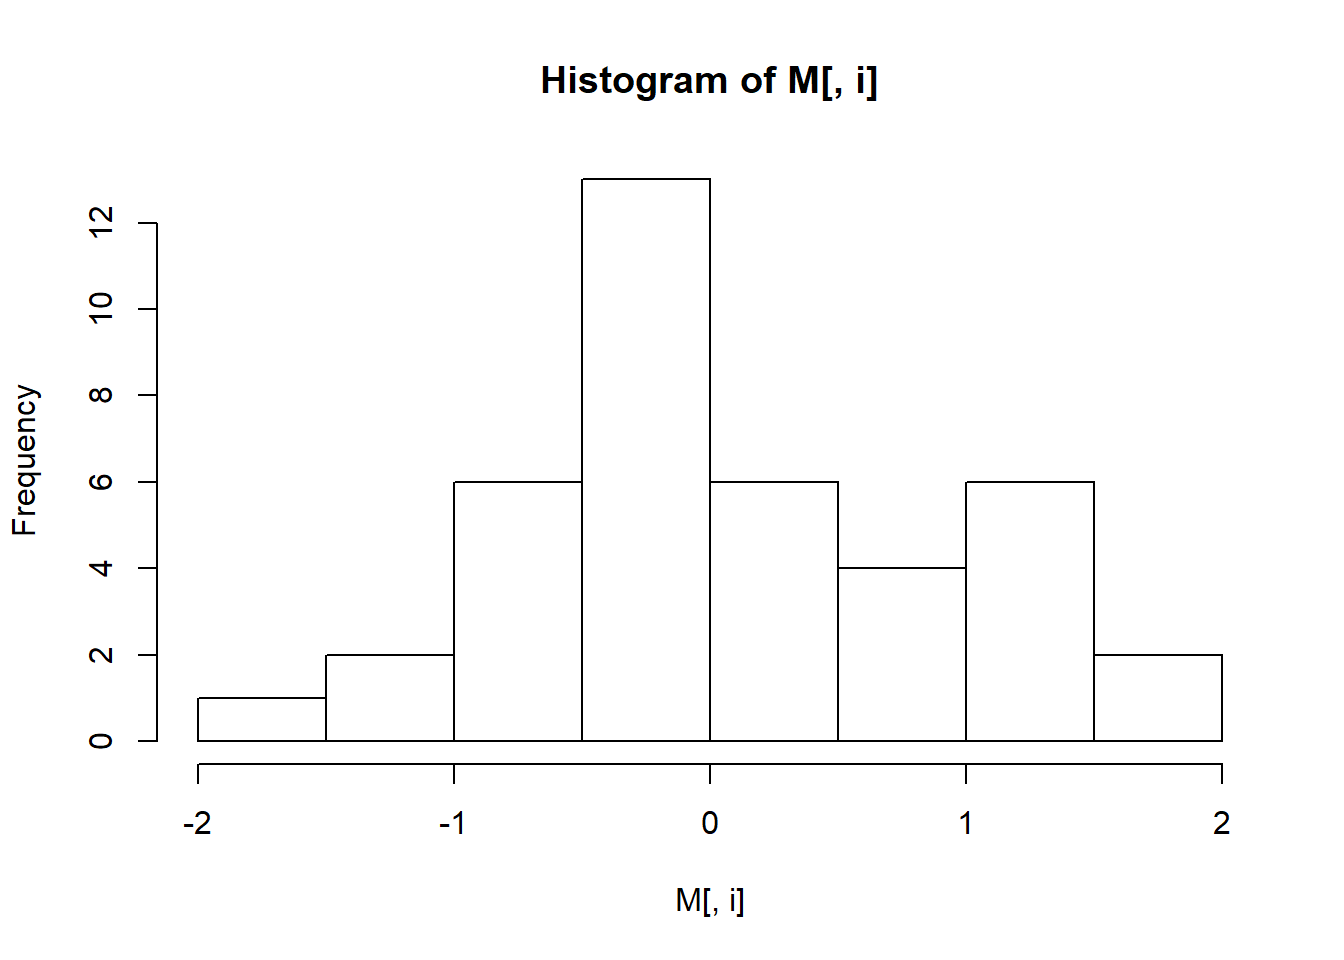
\includegraphics{plotandexplain_files/figure-latex/unnamed-chunk-3-1.pdf}
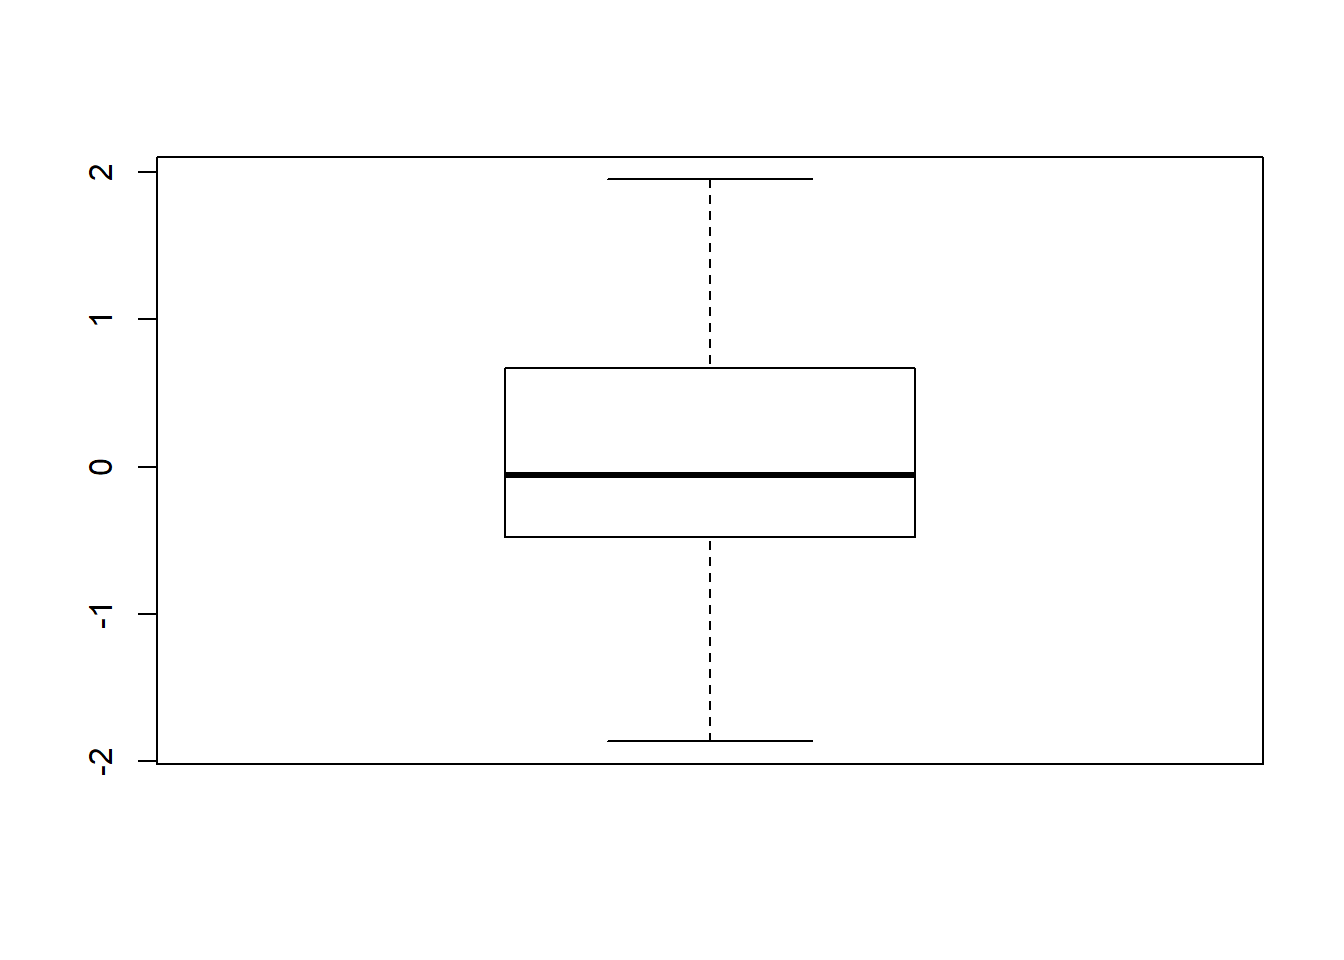
\includegraphics{plotandexplain_files/figure-latex/unnamed-chunk-3-2.pdf}
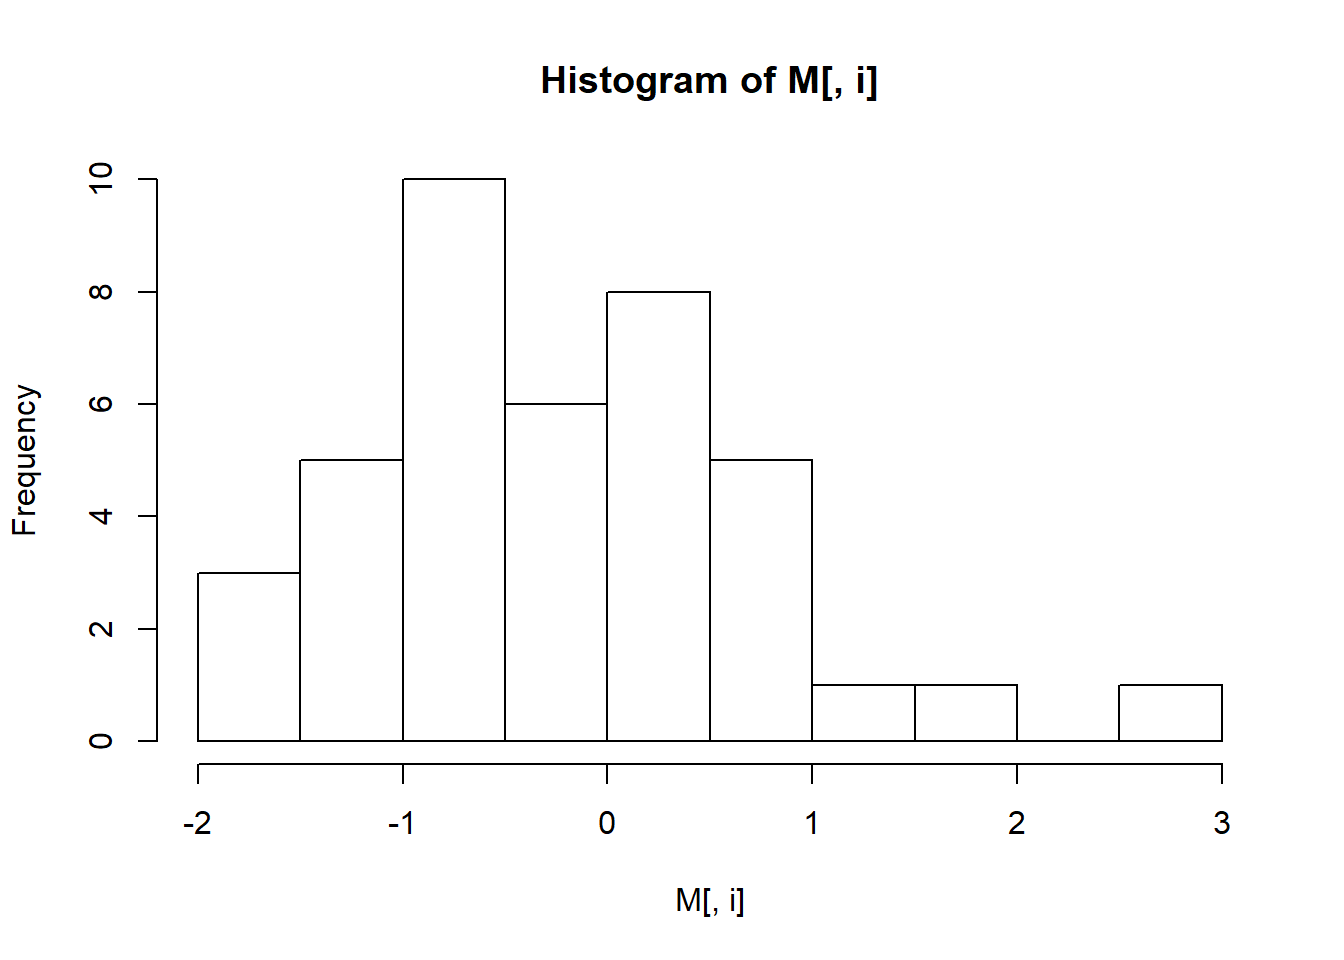
\includegraphics{plotandexplain_files/figure-latex/unnamed-chunk-3-3.pdf}
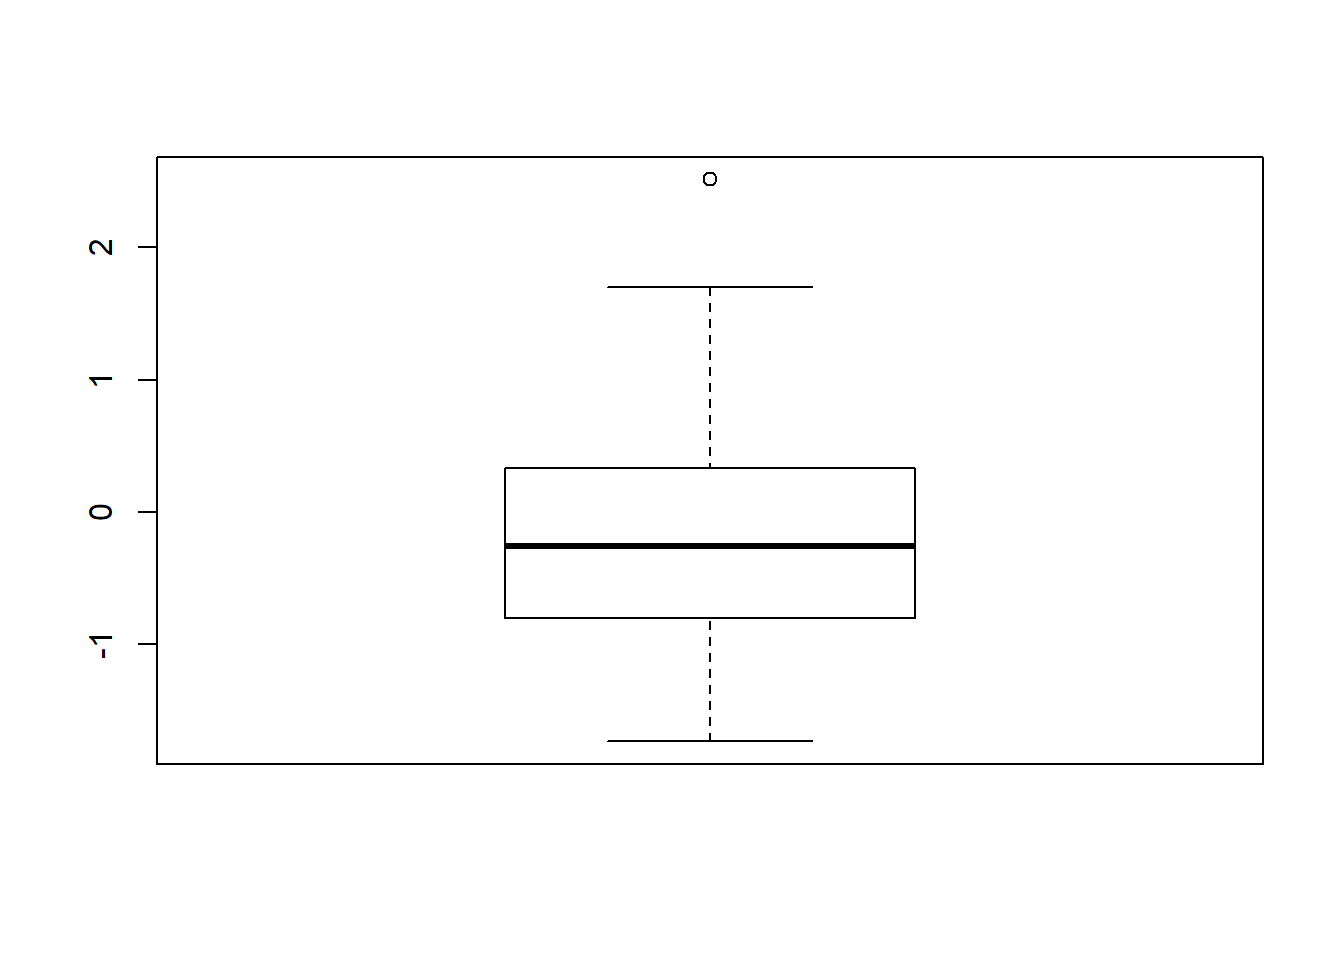
\includegraphics{plotandexplain_files/figure-latex/unnamed-chunk-3-4.pdf}
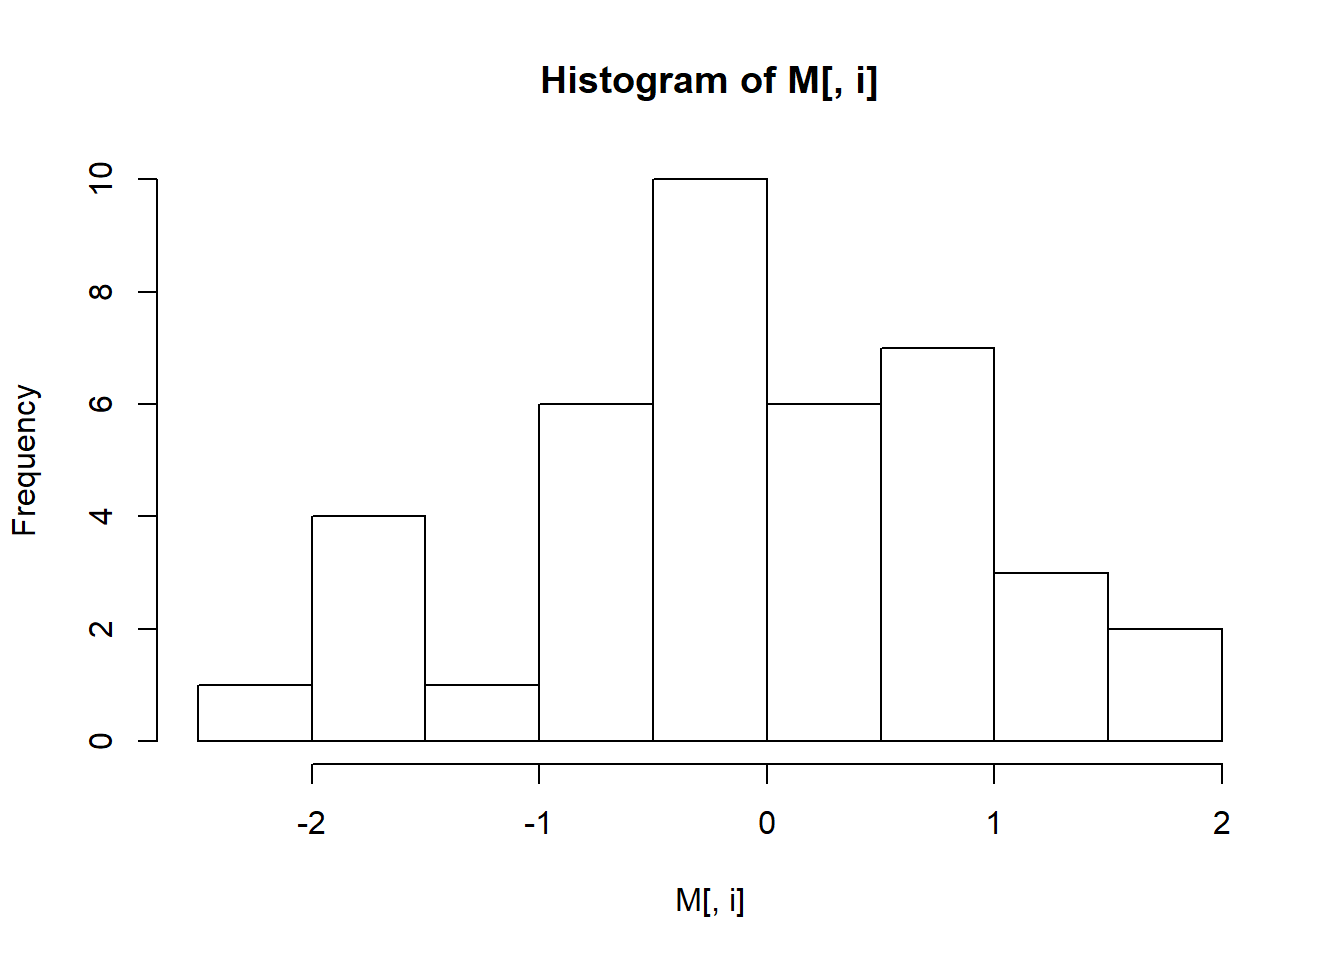
\includegraphics{plotandexplain_files/figure-latex/unnamed-chunk-3-5.pdf}
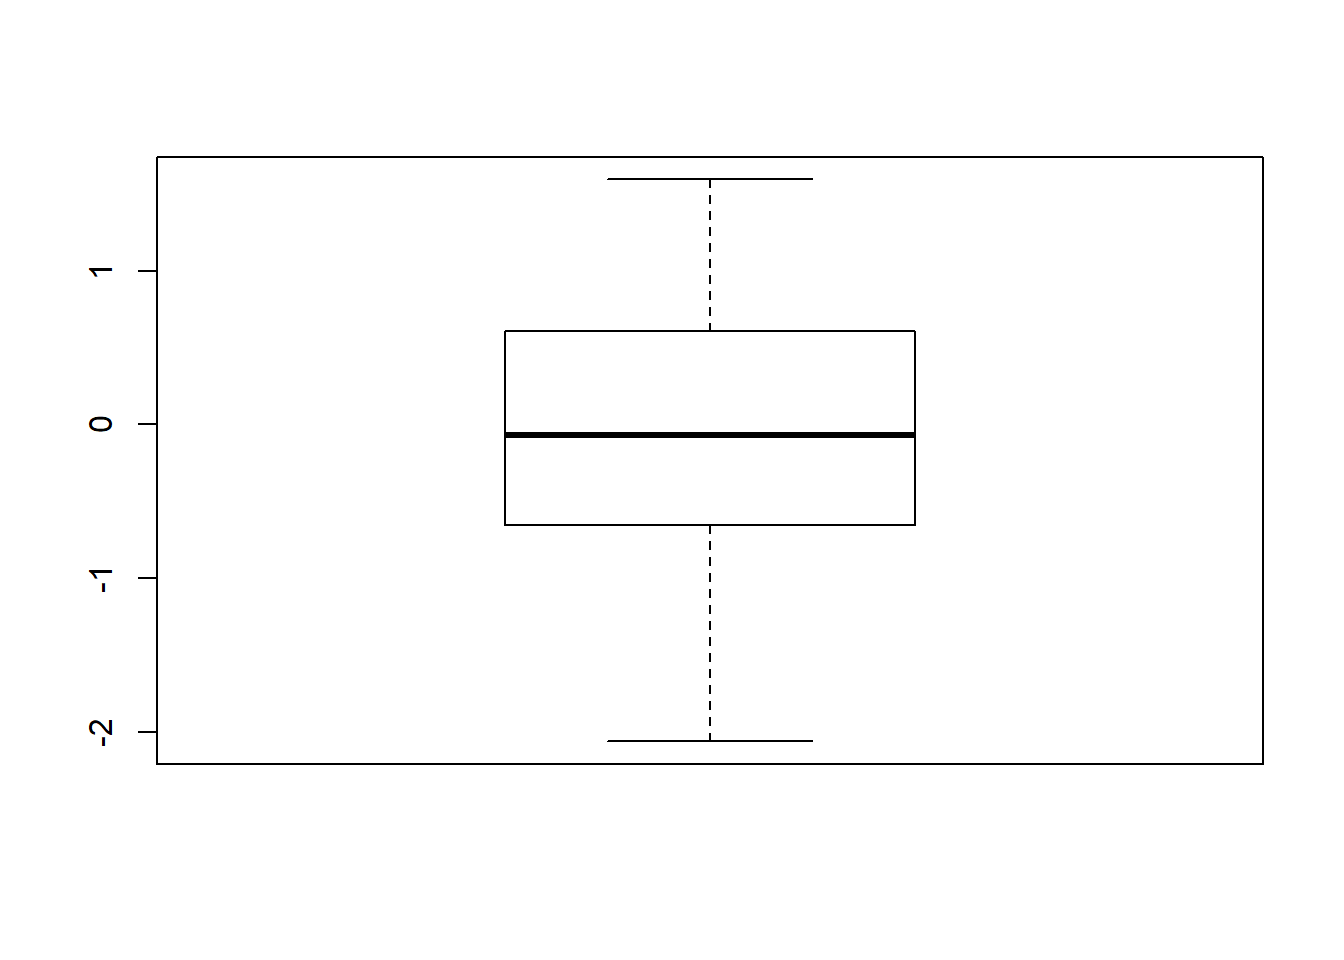
\includegraphics{plotandexplain_files/figure-latex/unnamed-chunk-3-6.pdf}
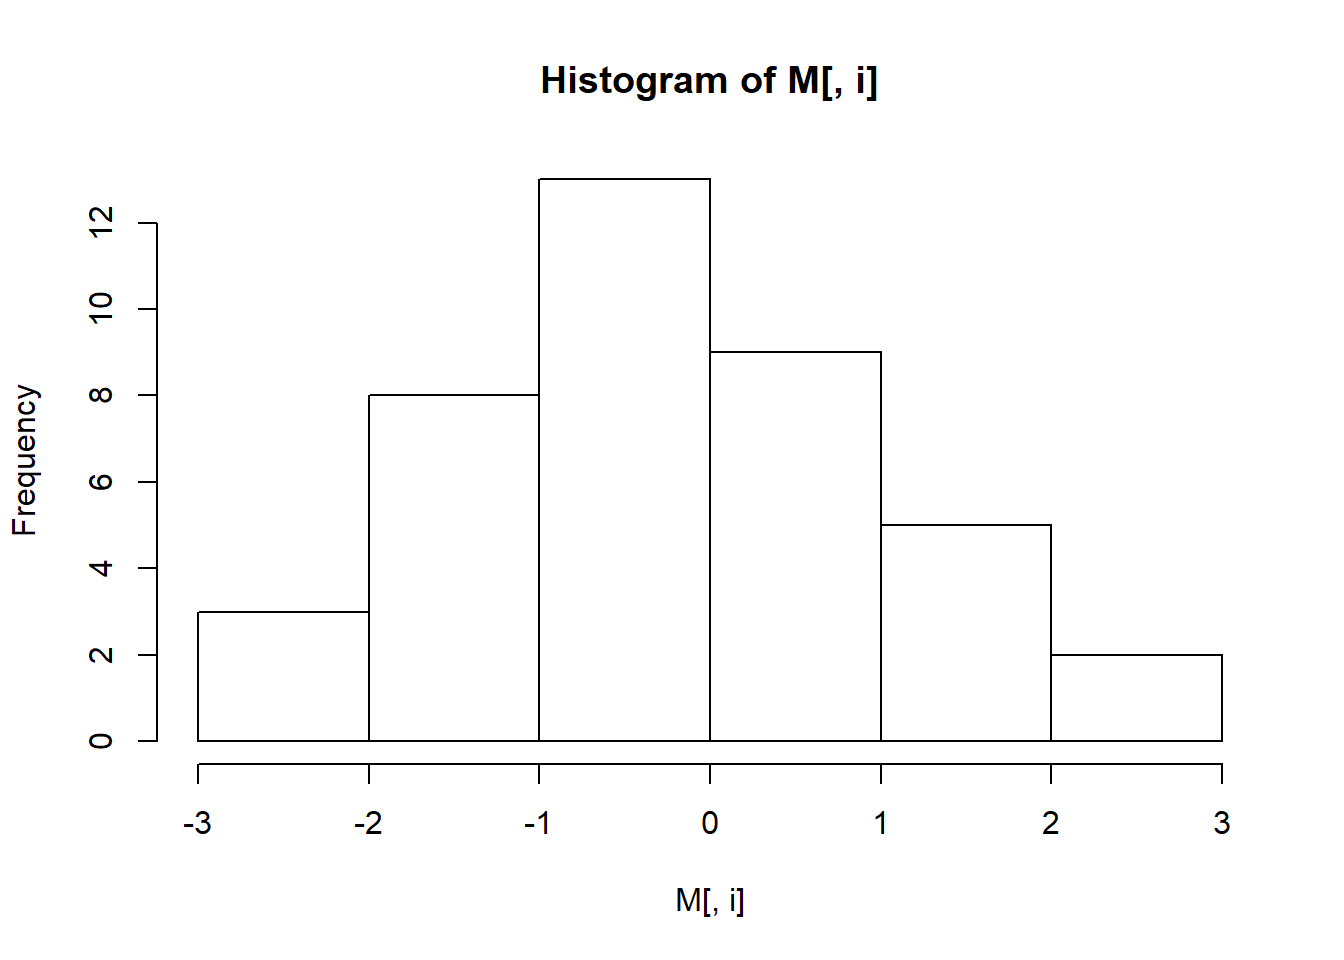
\includegraphics{plotandexplain_files/figure-latex/unnamed-chunk-3-7.pdf}
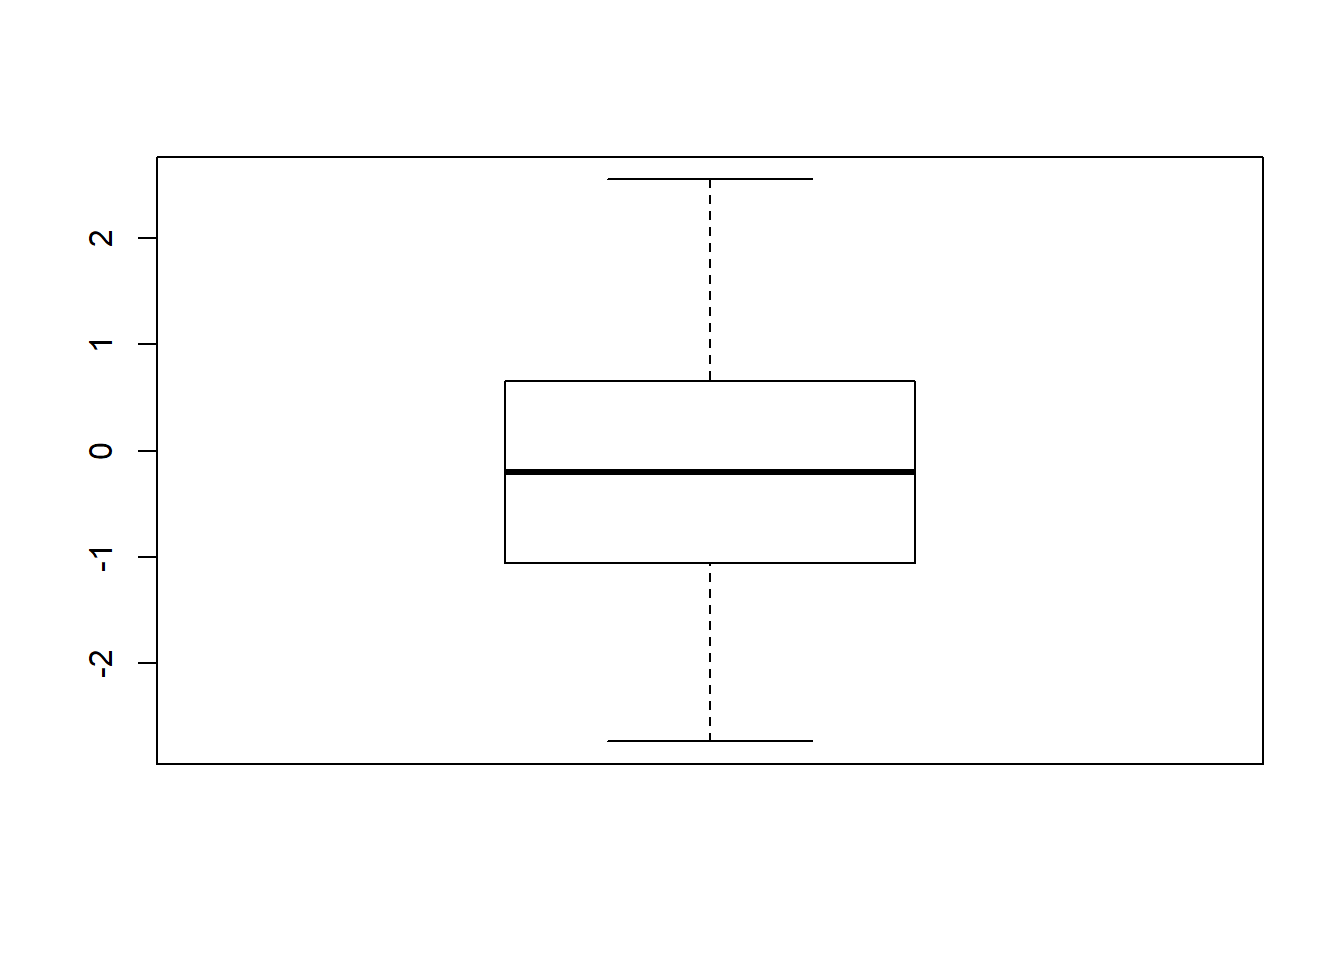
\includegraphics{plotandexplain_files/figure-latex/unnamed-chunk-3-8.pdf}
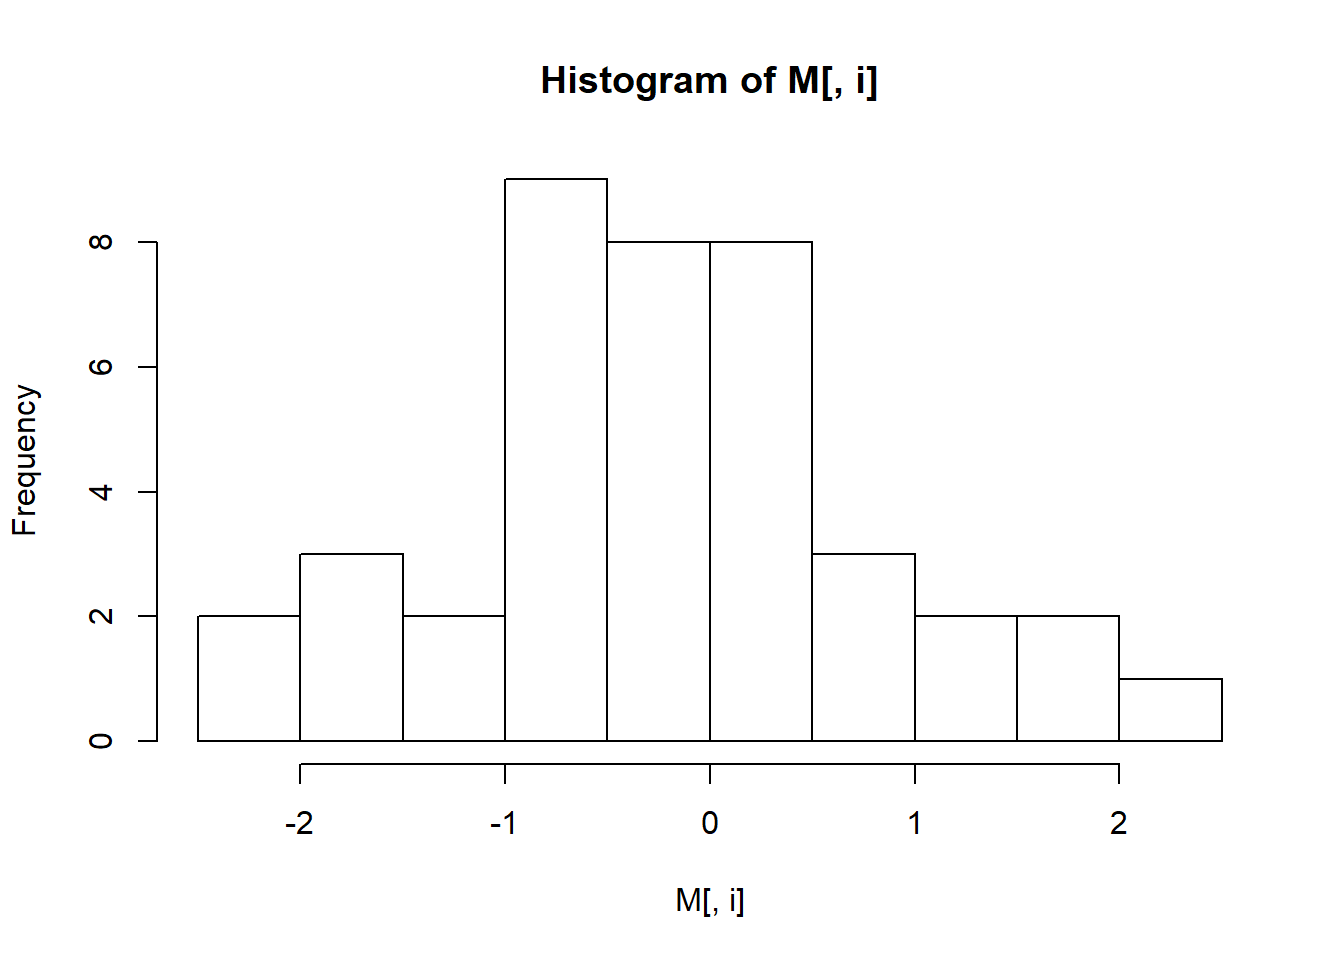
\includegraphics{plotandexplain_files/figure-latex/unnamed-chunk-3-9.pdf}
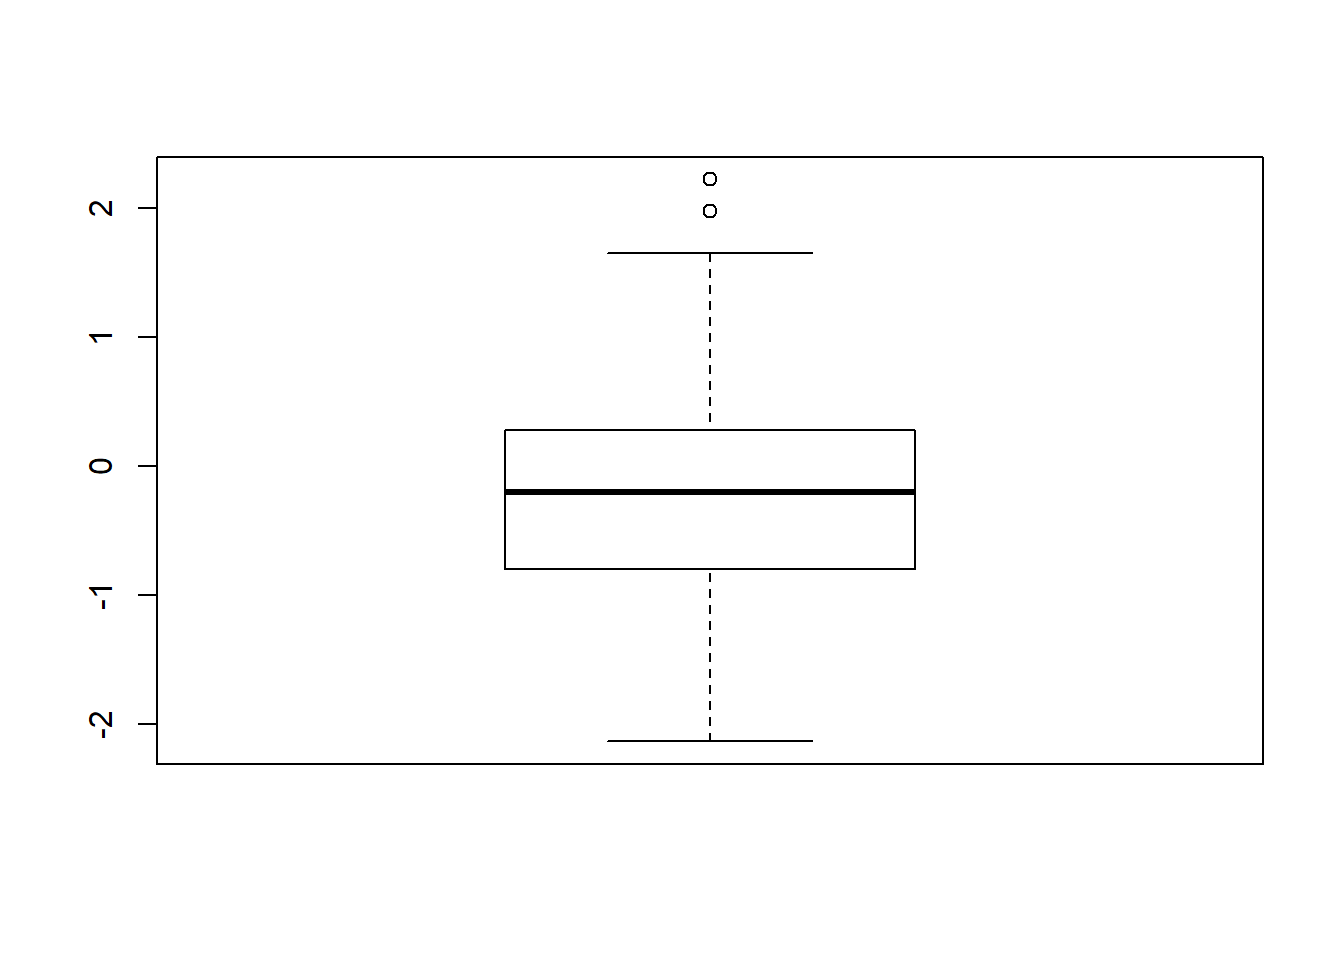
\includegraphics{plotandexplain_files/figure-latex/unnamed-chunk-3-10.pdf}
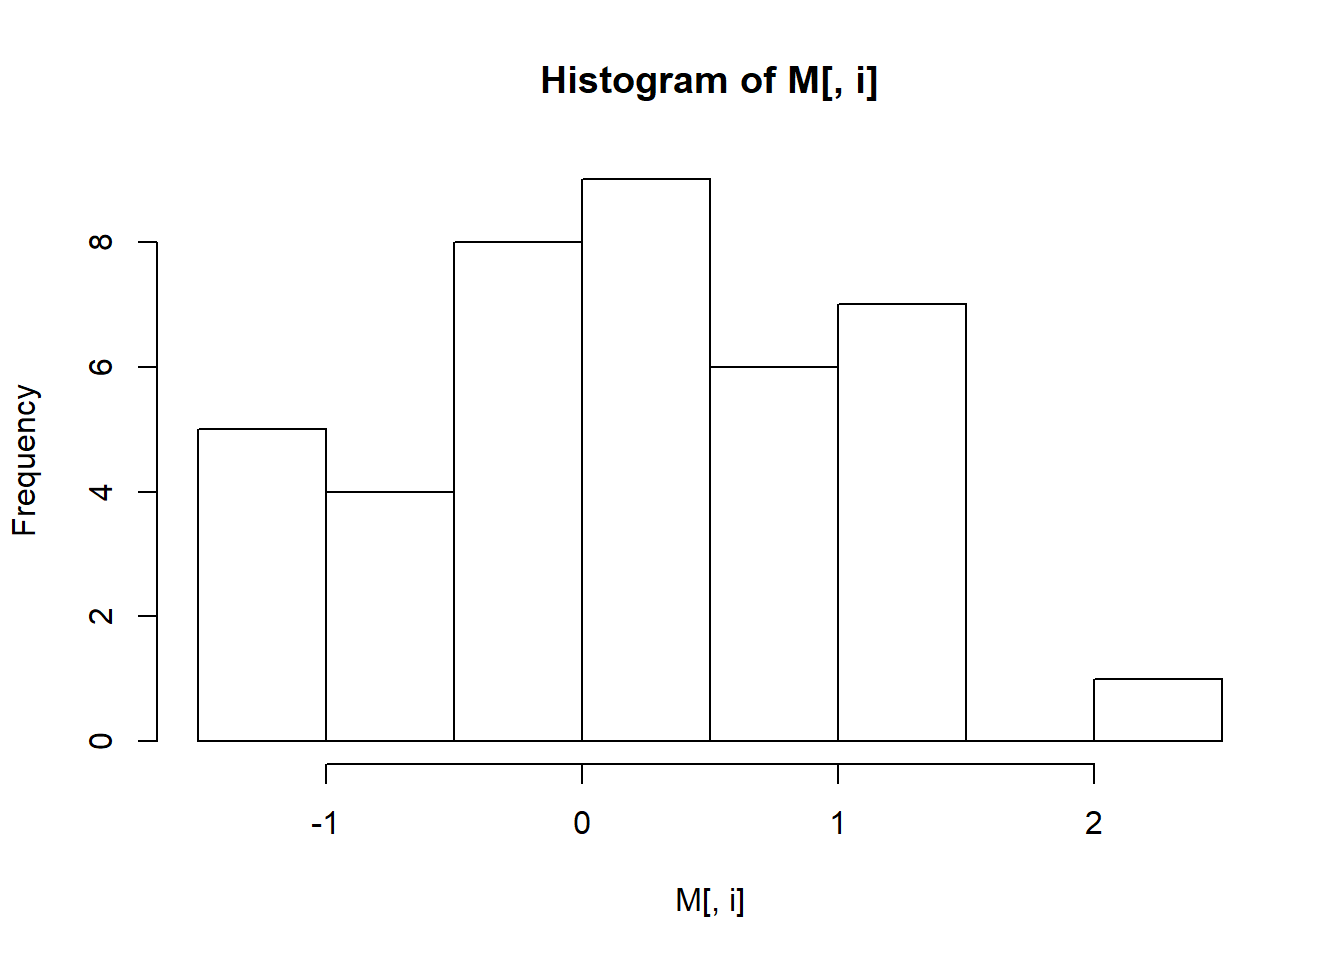
\includegraphics{plotandexplain_files/figure-latex/unnamed-chunk-3-11.pdf}
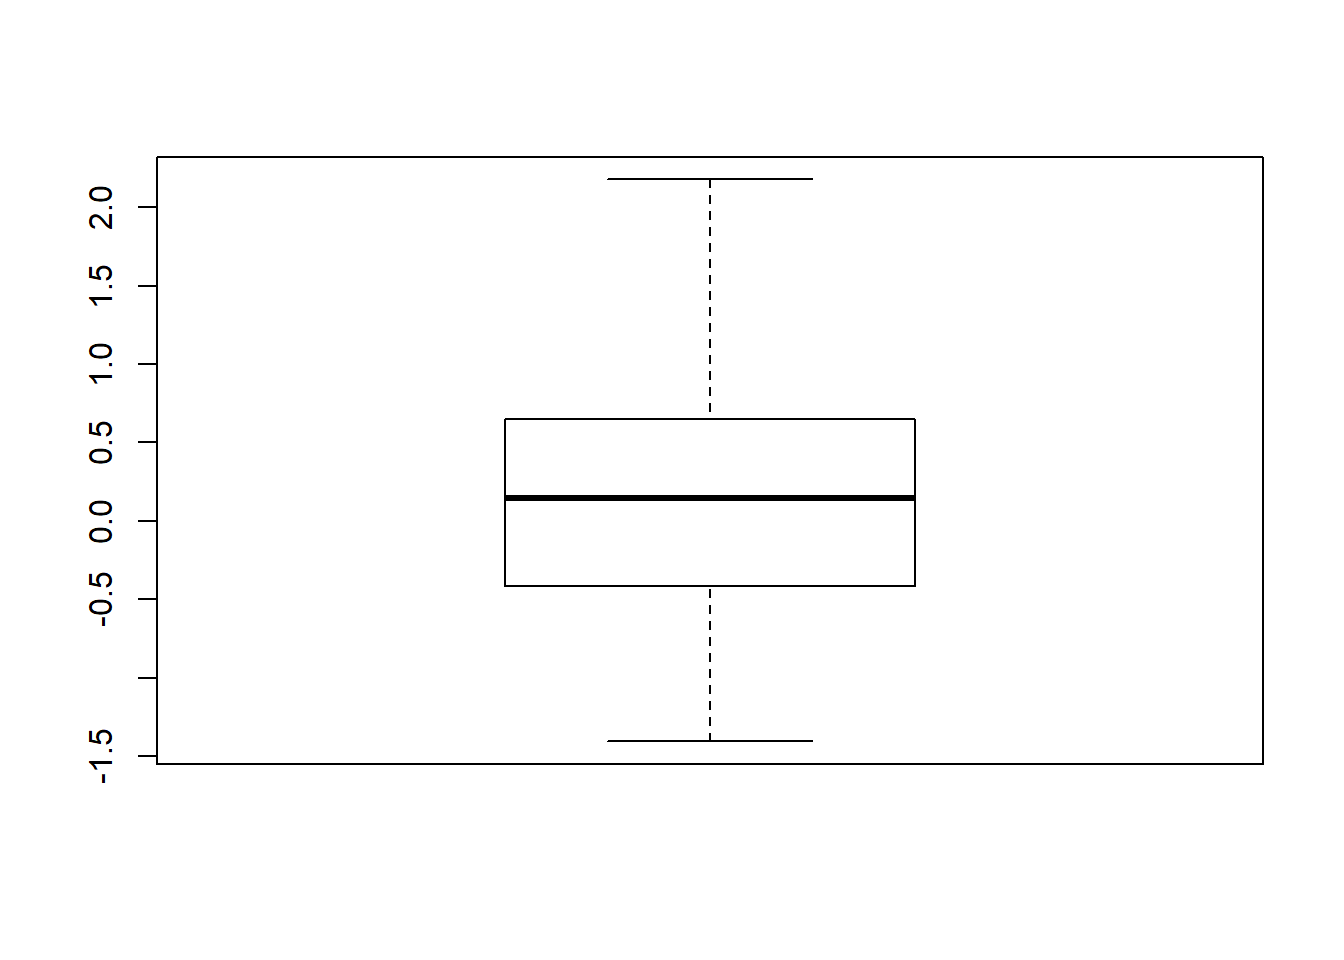
\includegraphics{plotandexplain_files/figure-latex/unnamed-chunk-3-12.pdf}
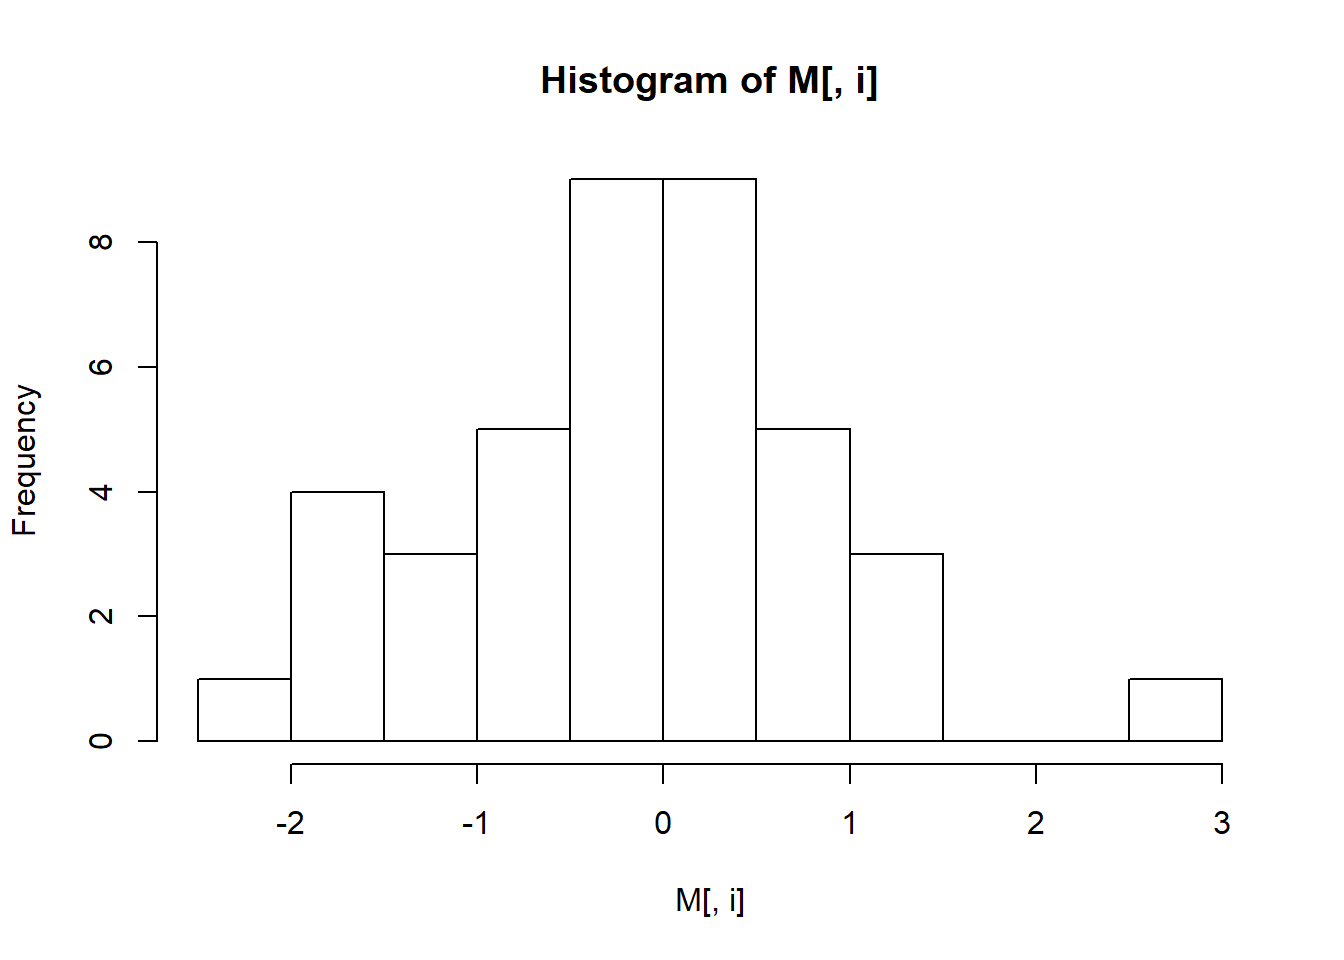
\includegraphics{plotandexplain_files/figure-latex/unnamed-chunk-3-13.pdf}
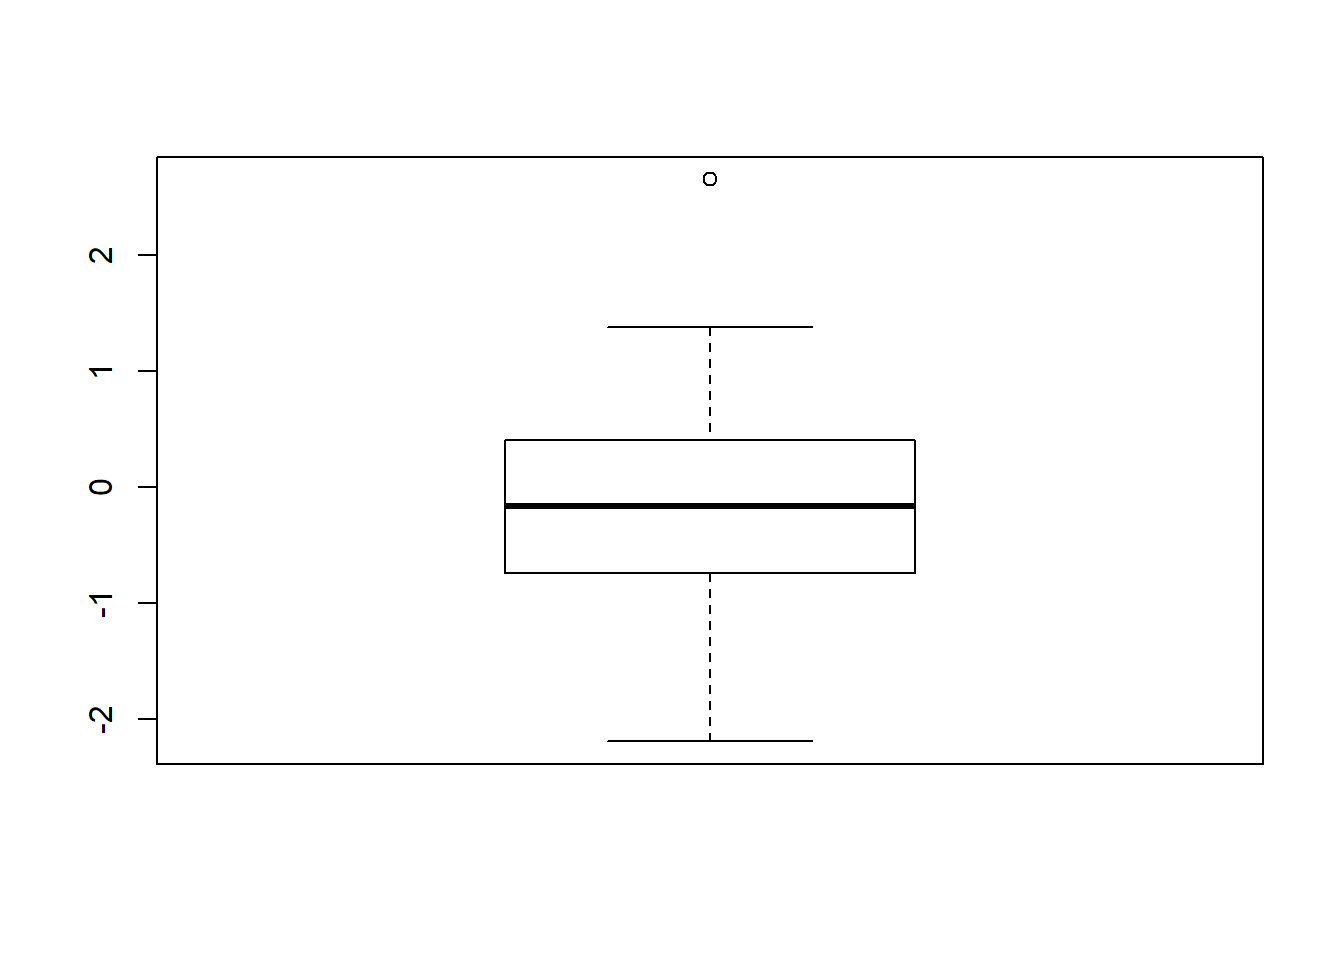
\includegraphics{plotandexplain_files/figure-latex/unnamed-chunk-3-14.pdf}
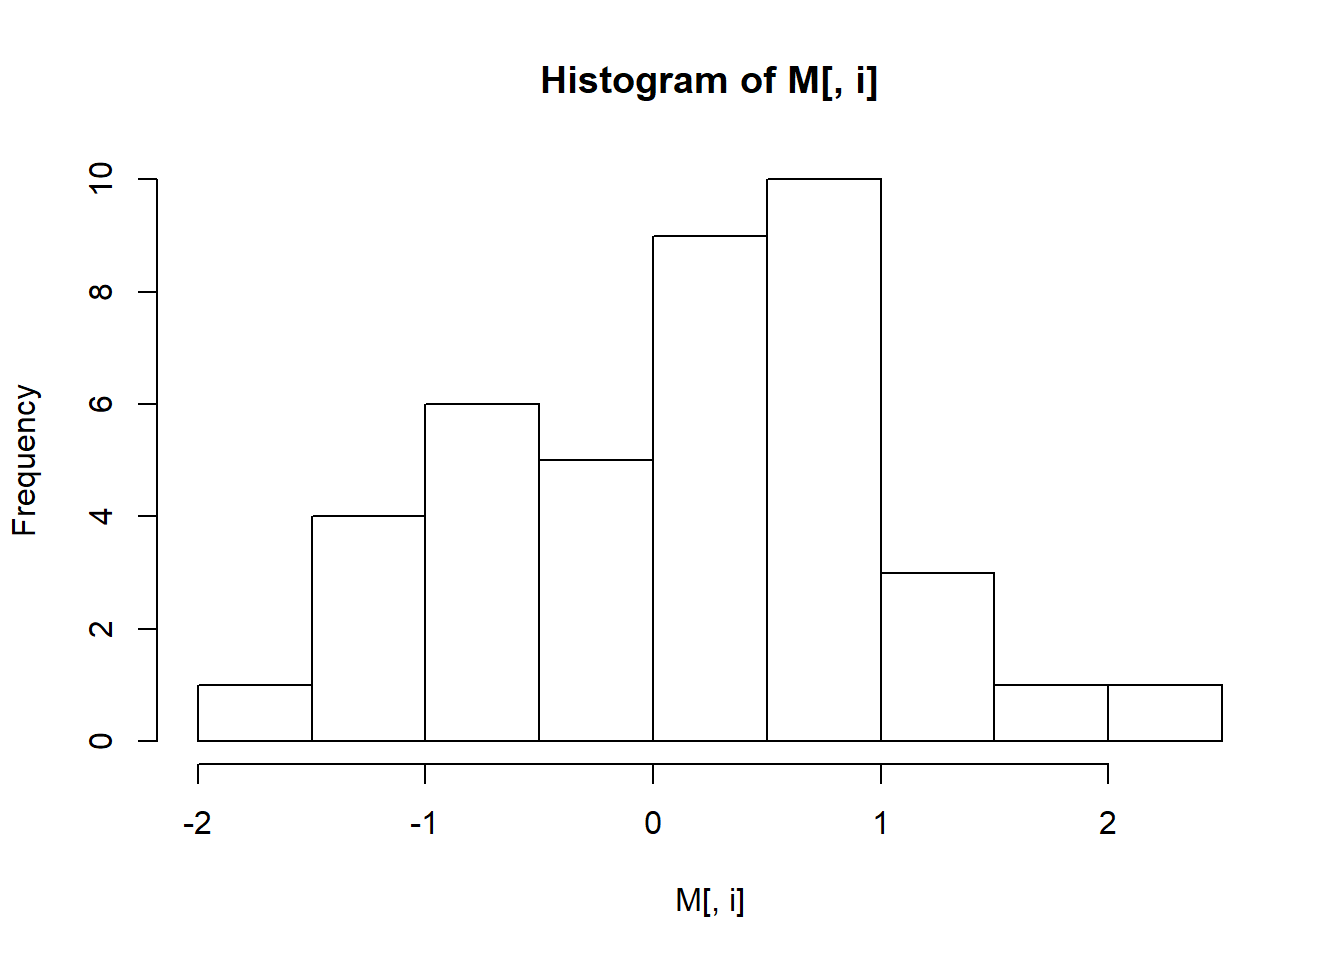
\includegraphics{plotandexplain_files/figure-latex/unnamed-chunk-3-15.pdf}
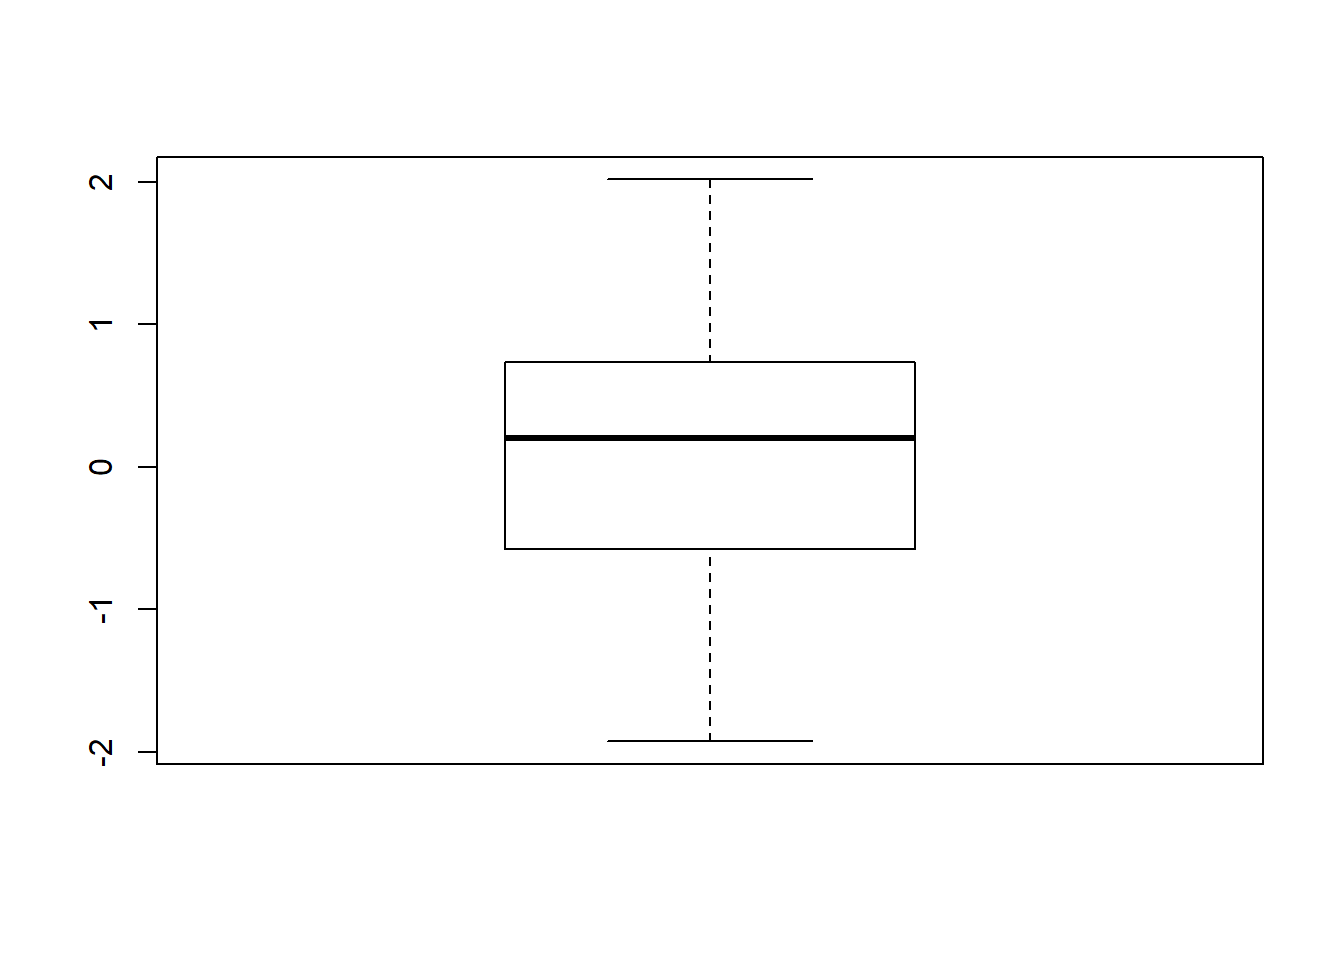
\includegraphics{plotandexplain_files/figure-latex/unnamed-chunk-3-16.pdf}
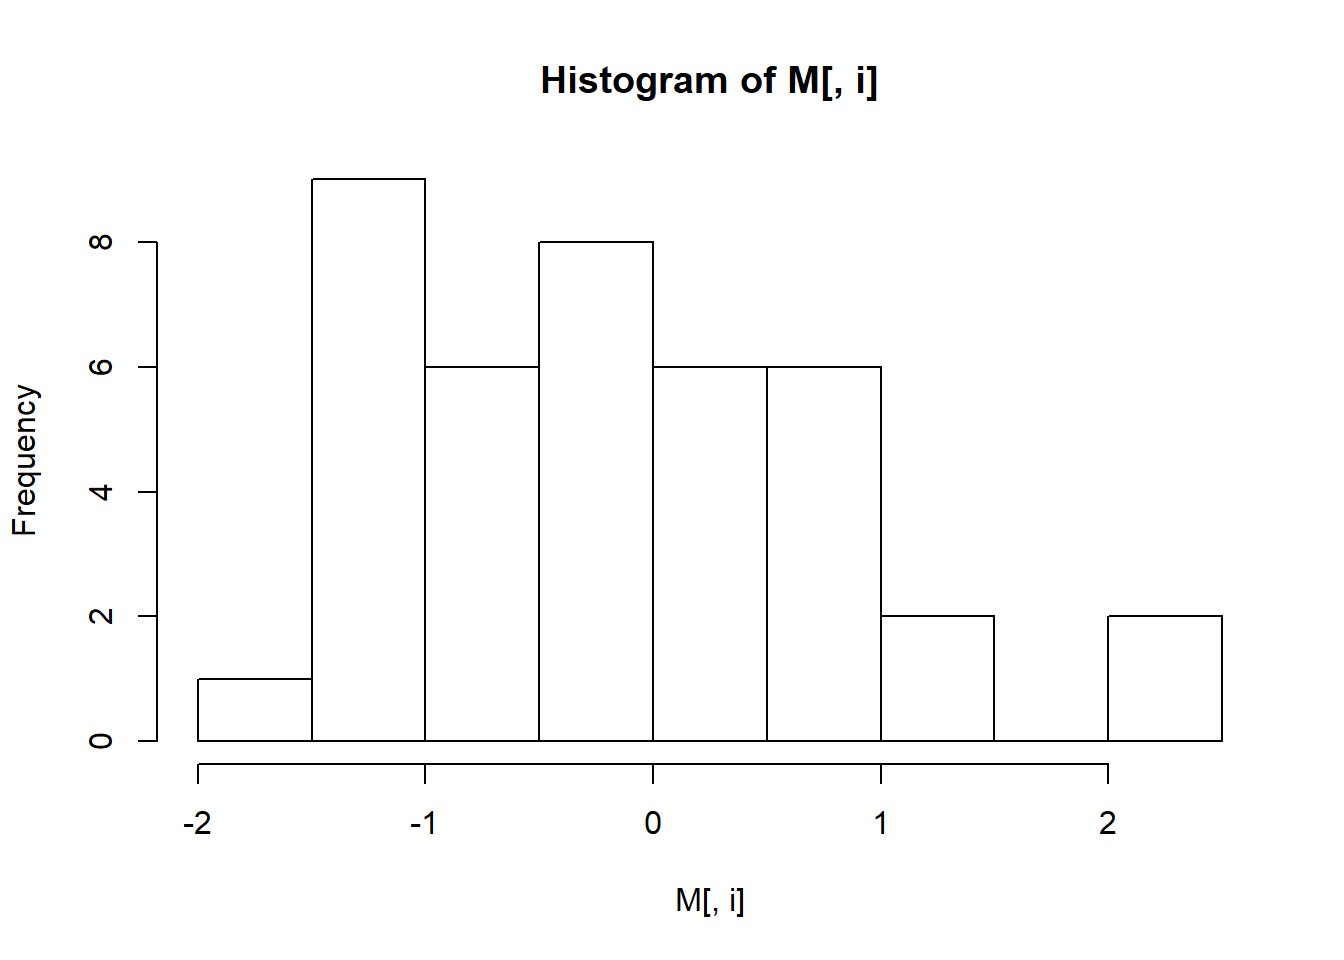
\includegraphics{plotandexplain_files/figure-latex/unnamed-chunk-3-17.pdf}
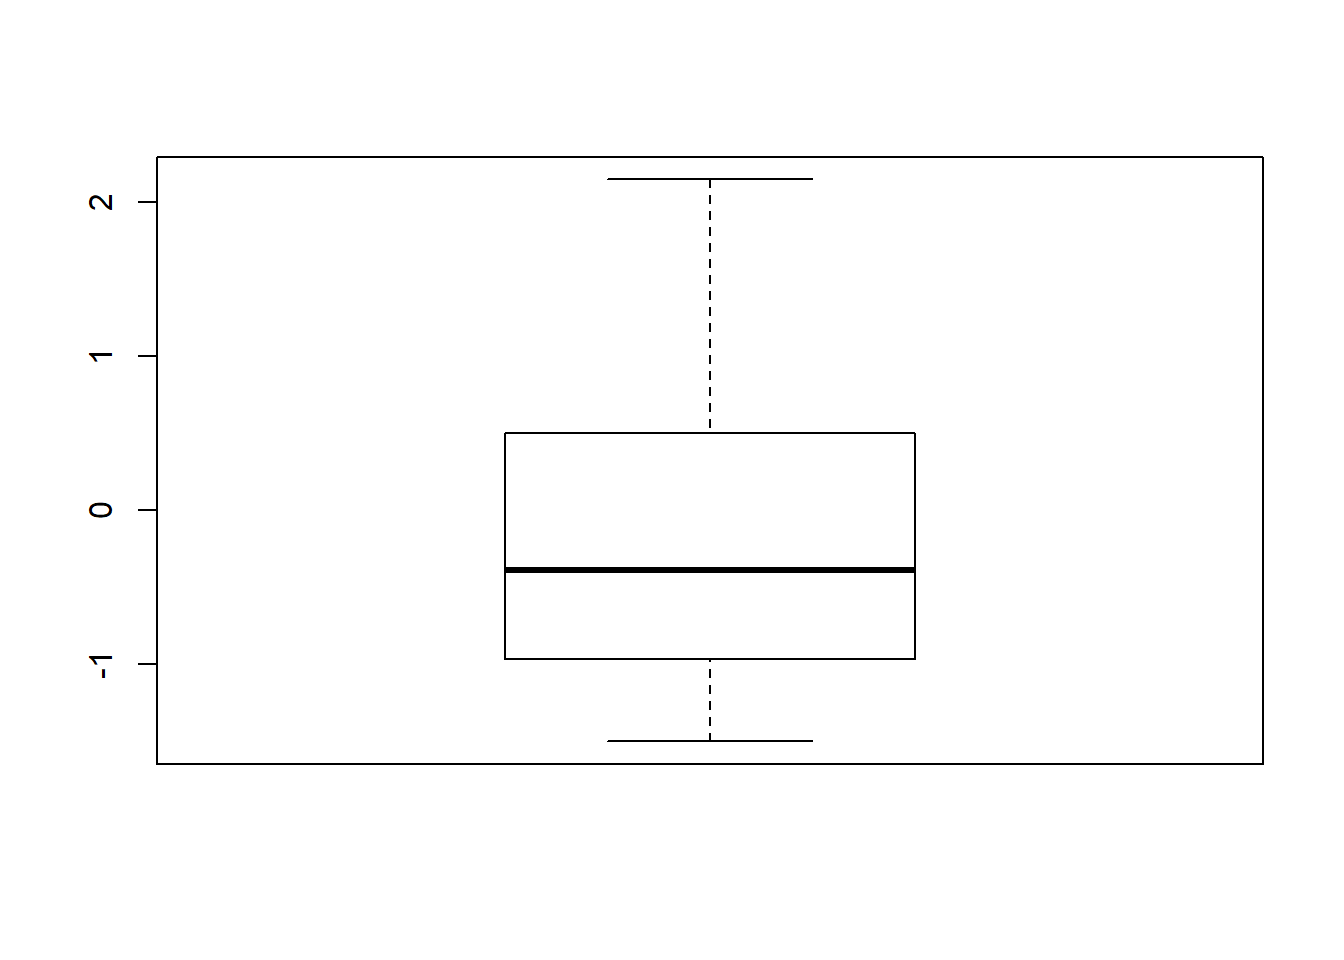
\includegraphics{plotandexplain_files/figure-latex/unnamed-chunk-3-18.pdf}
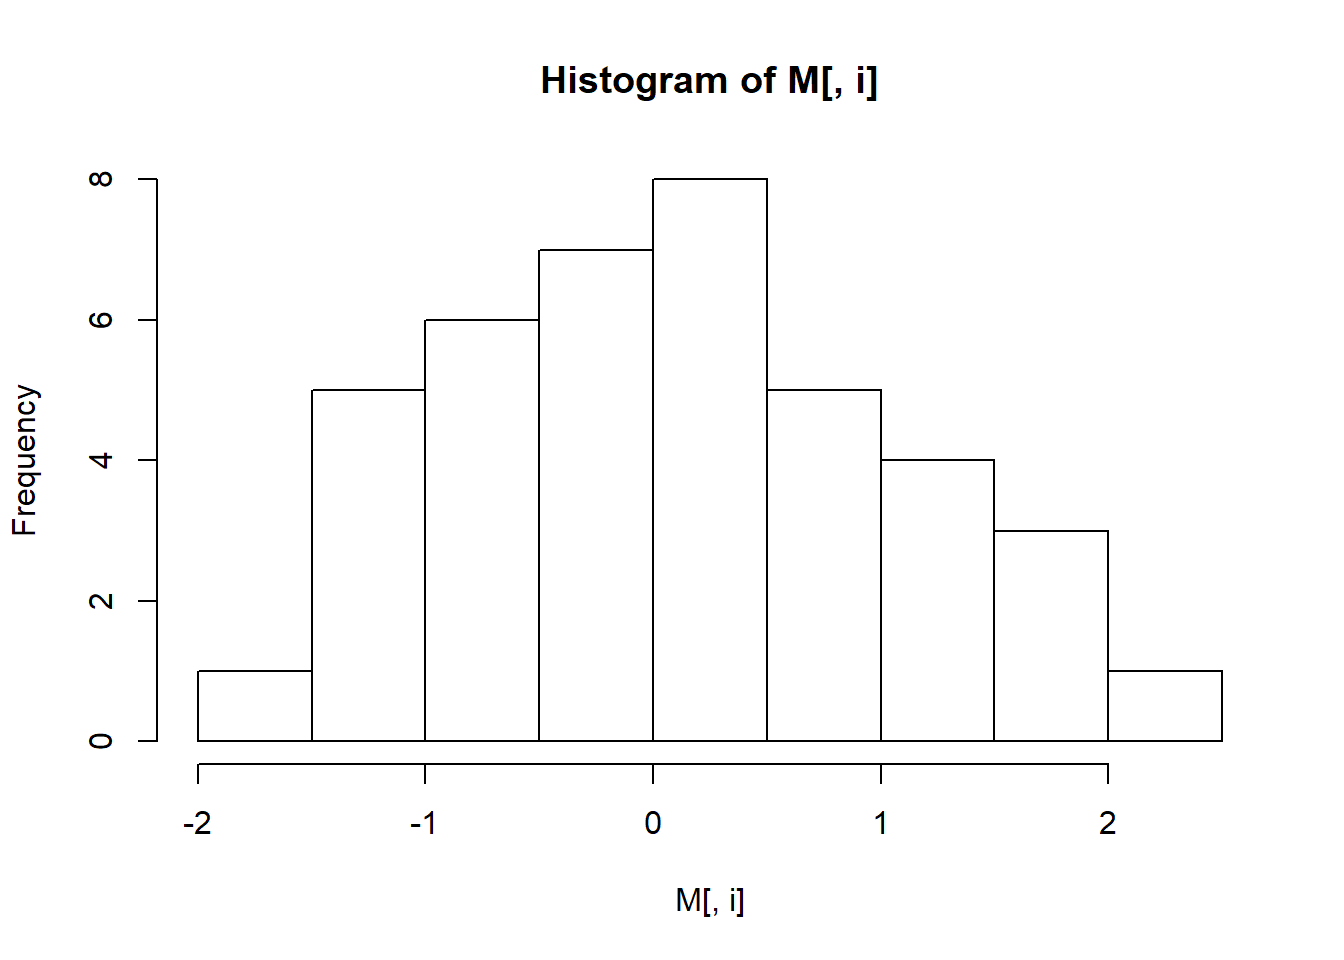
\includegraphics{plotandexplain_files/figure-latex/unnamed-chunk-3-19.pdf}
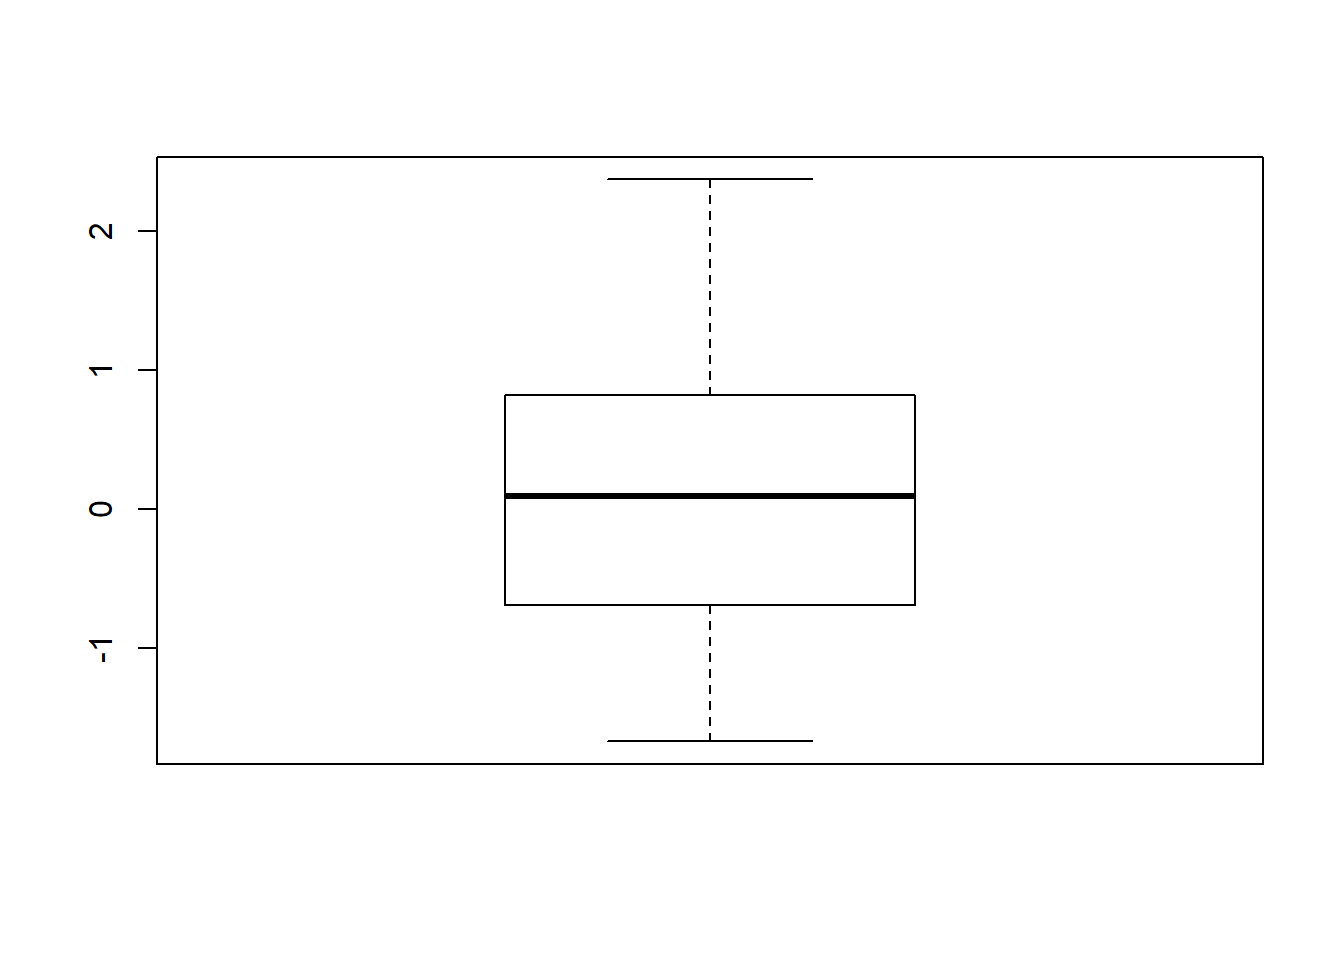
\includegraphics{plotandexplain_files/figure-latex/unnamed-chunk-3-20.pdf}
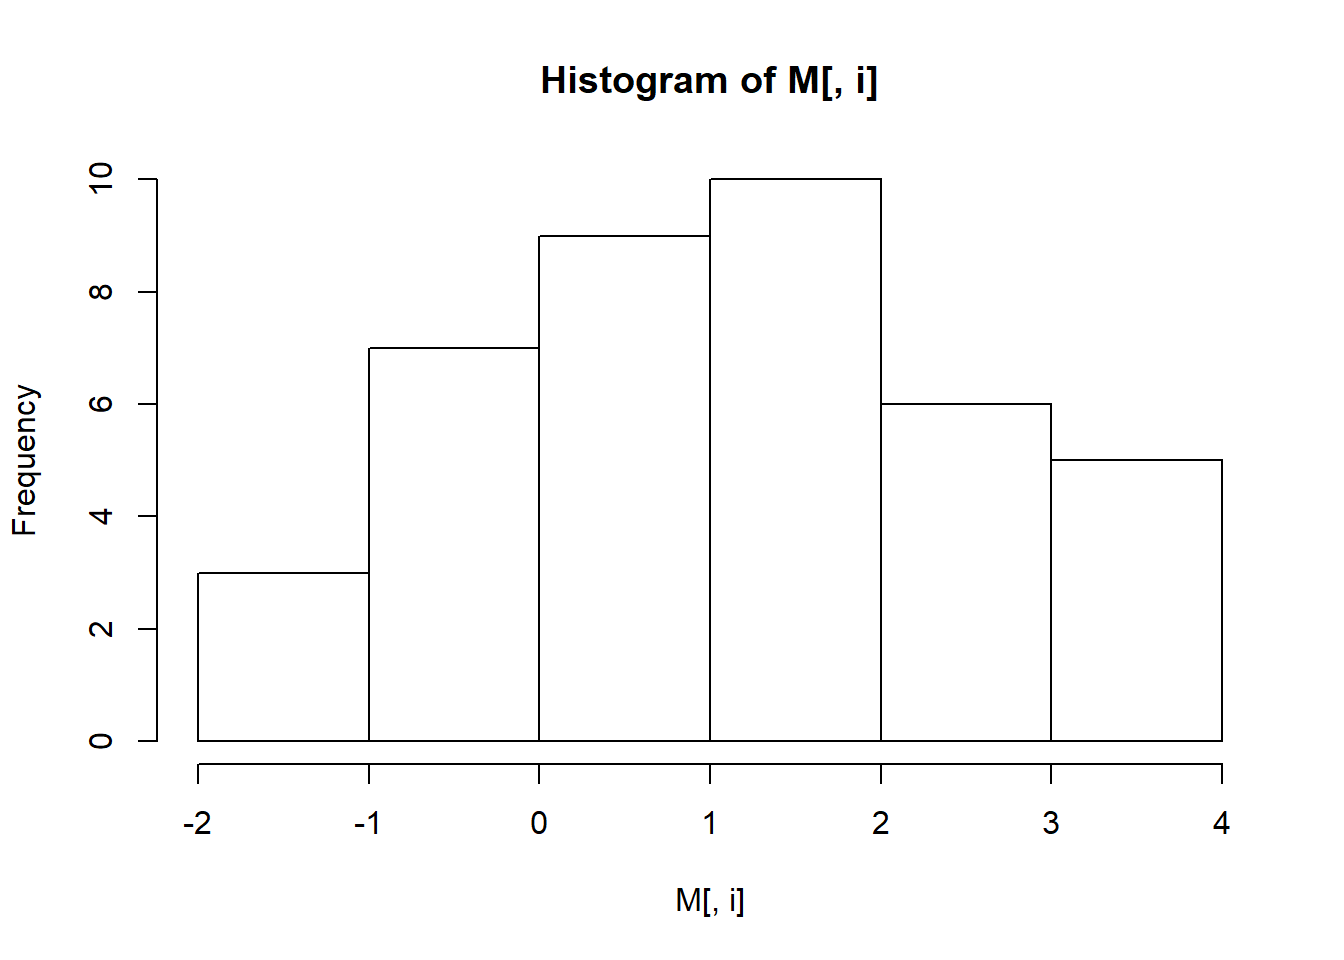
\includegraphics{plotandexplain_files/figure-latex/unnamed-chunk-3-21.pdf}
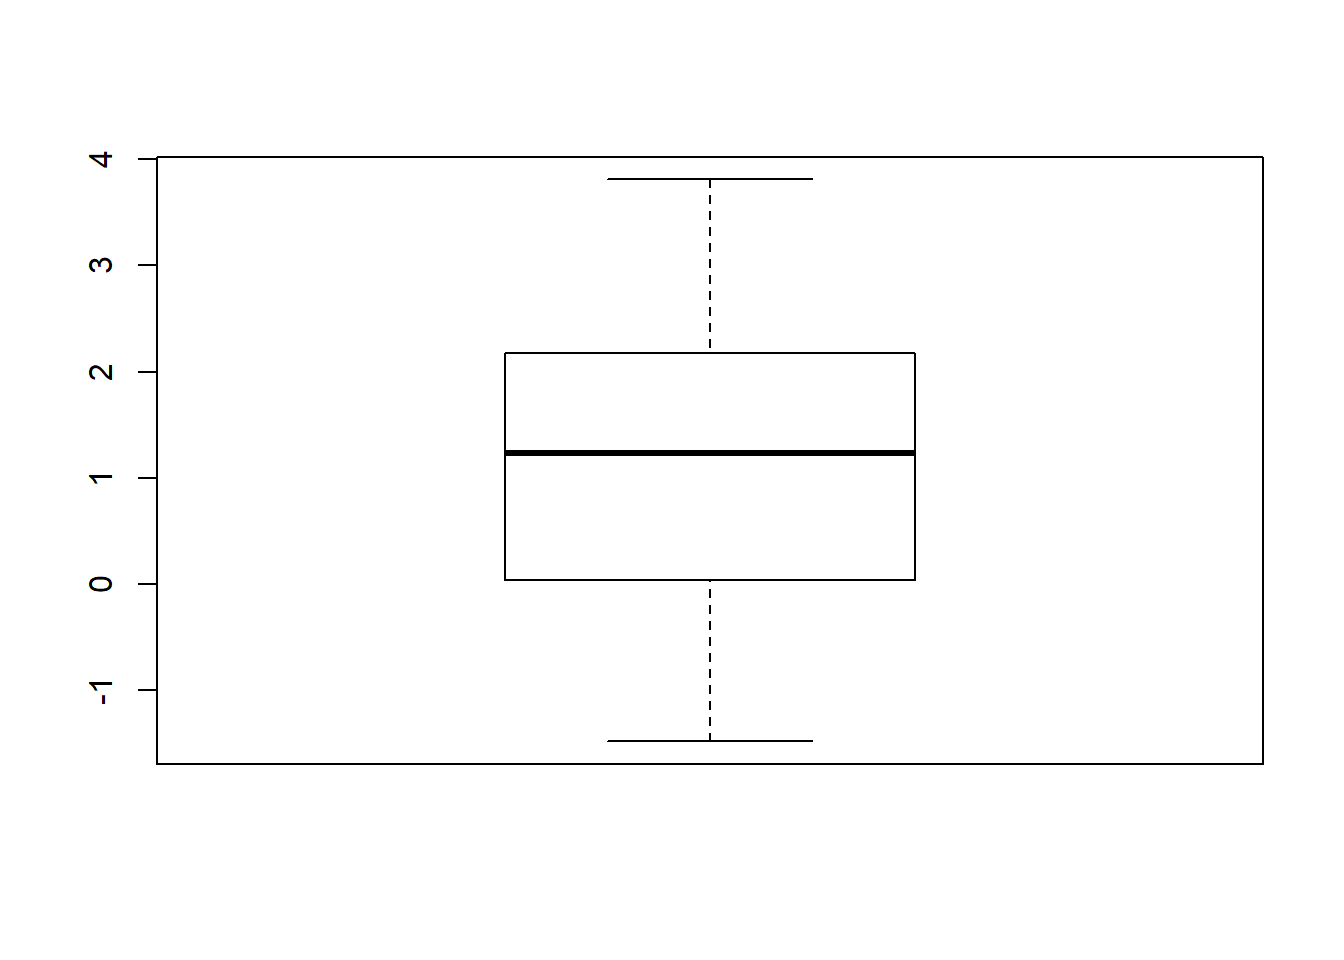
\includegraphics{plotandexplain_files/figure-latex/unnamed-chunk-3-22.pdf}
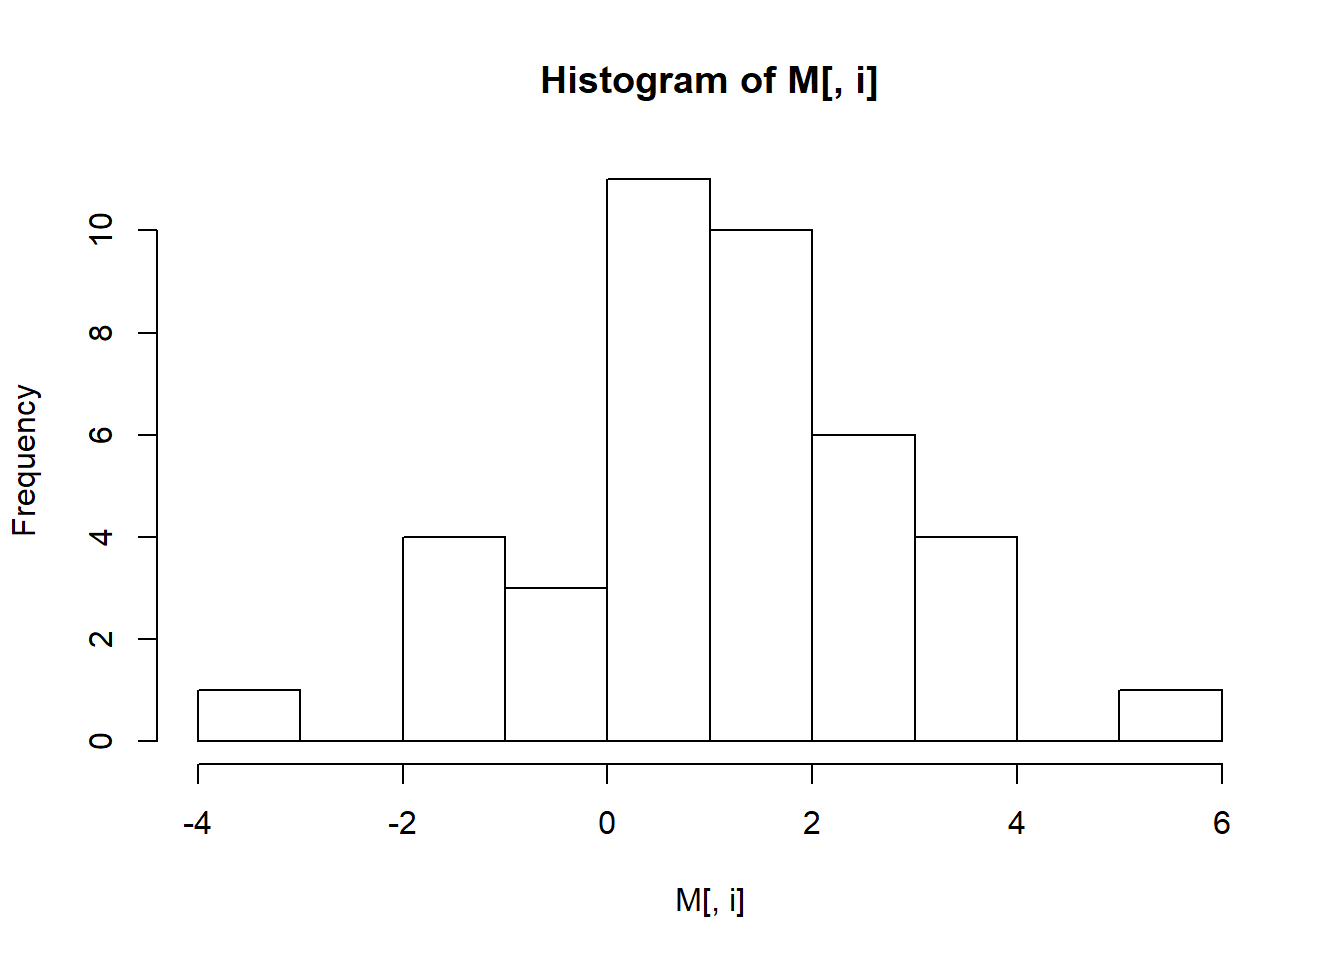
\includegraphics{plotandexplain_files/figure-latex/unnamed-chunk-3-23.pdf}
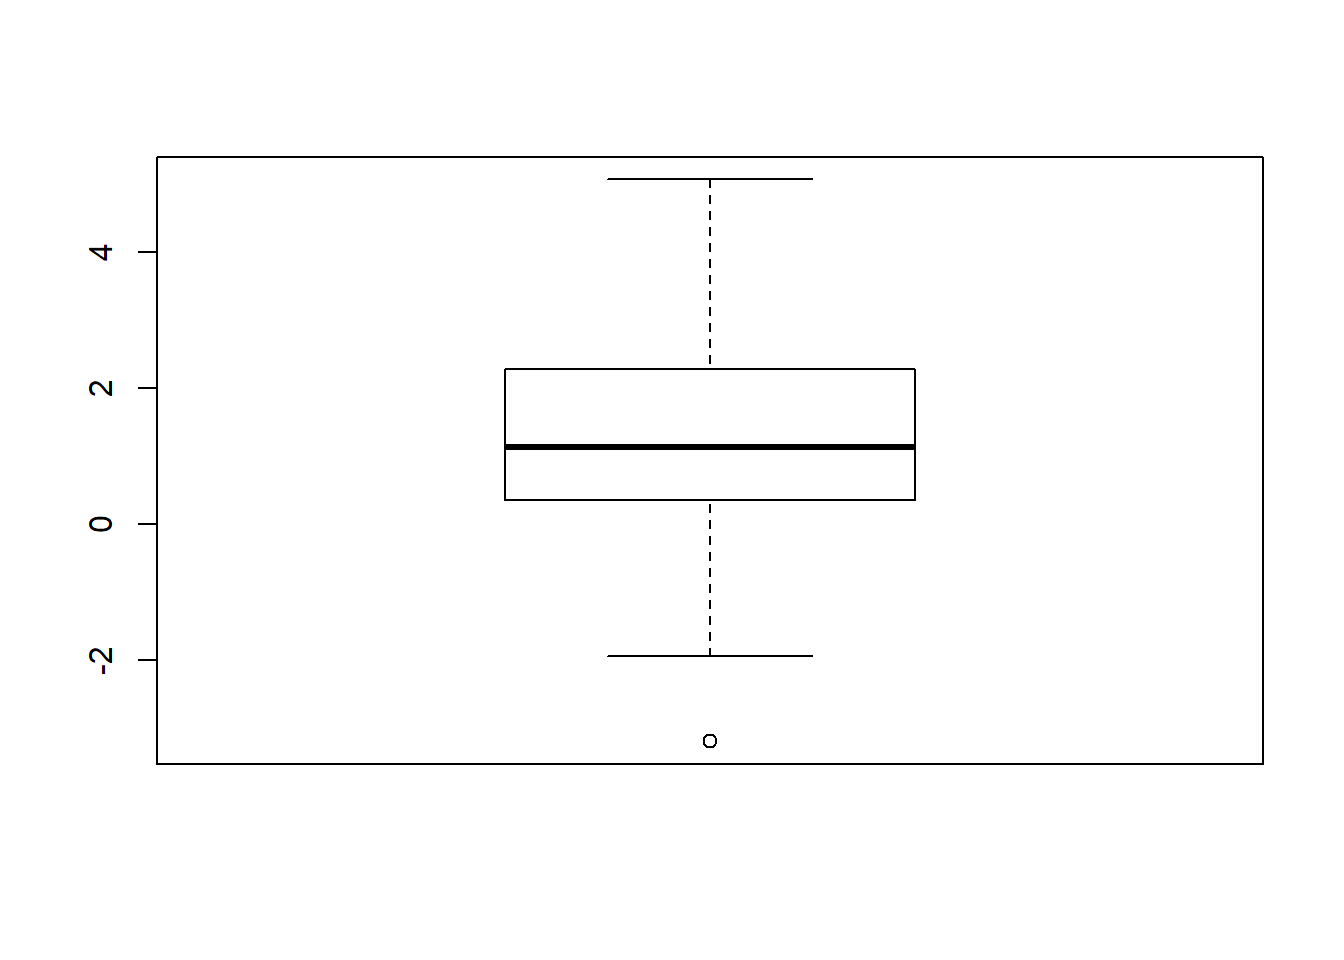
\includegraphics{plotandexplain_files/figure-latex/unnamed-chunk-3-24.pdf}
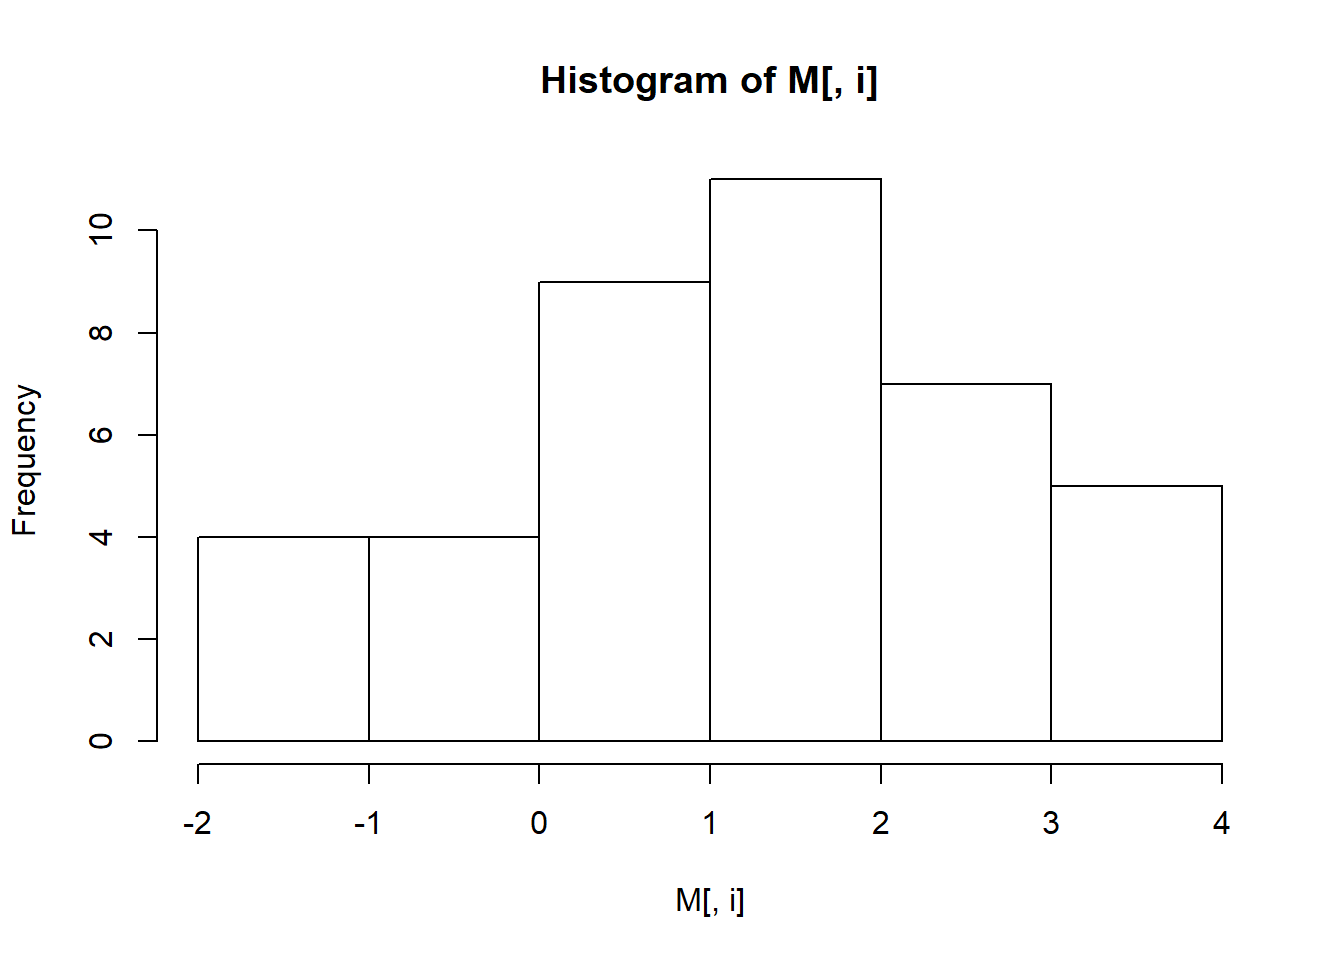
\includegraphics{plotandexplain_files/figure-latex/unnamed-chunk-3-25.pdf}
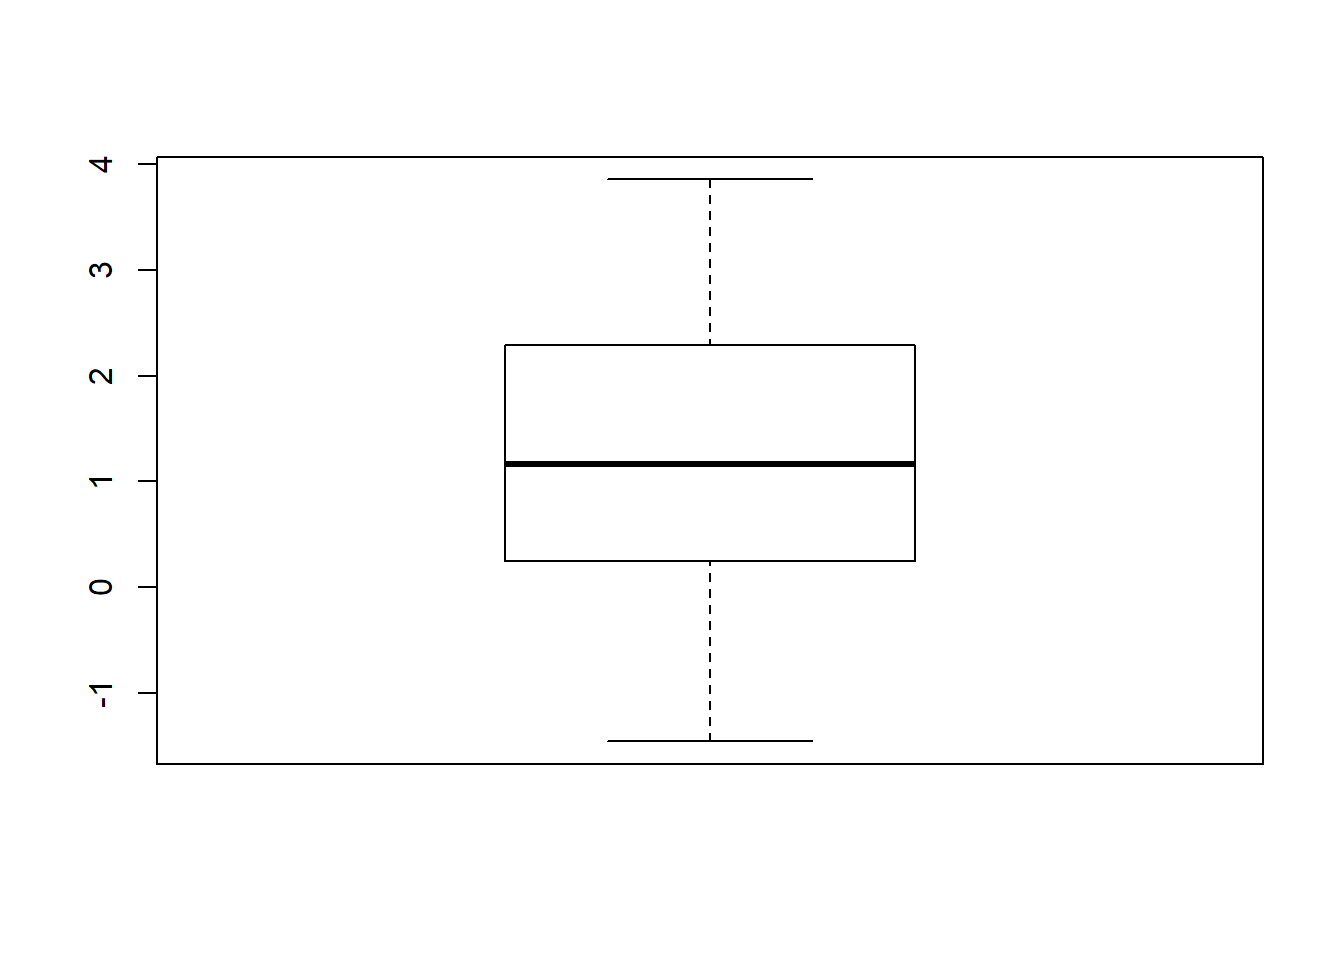
\includegraphics{plotandexplain_files/figure-latex/unnamed-chunk-3-26.pdf}
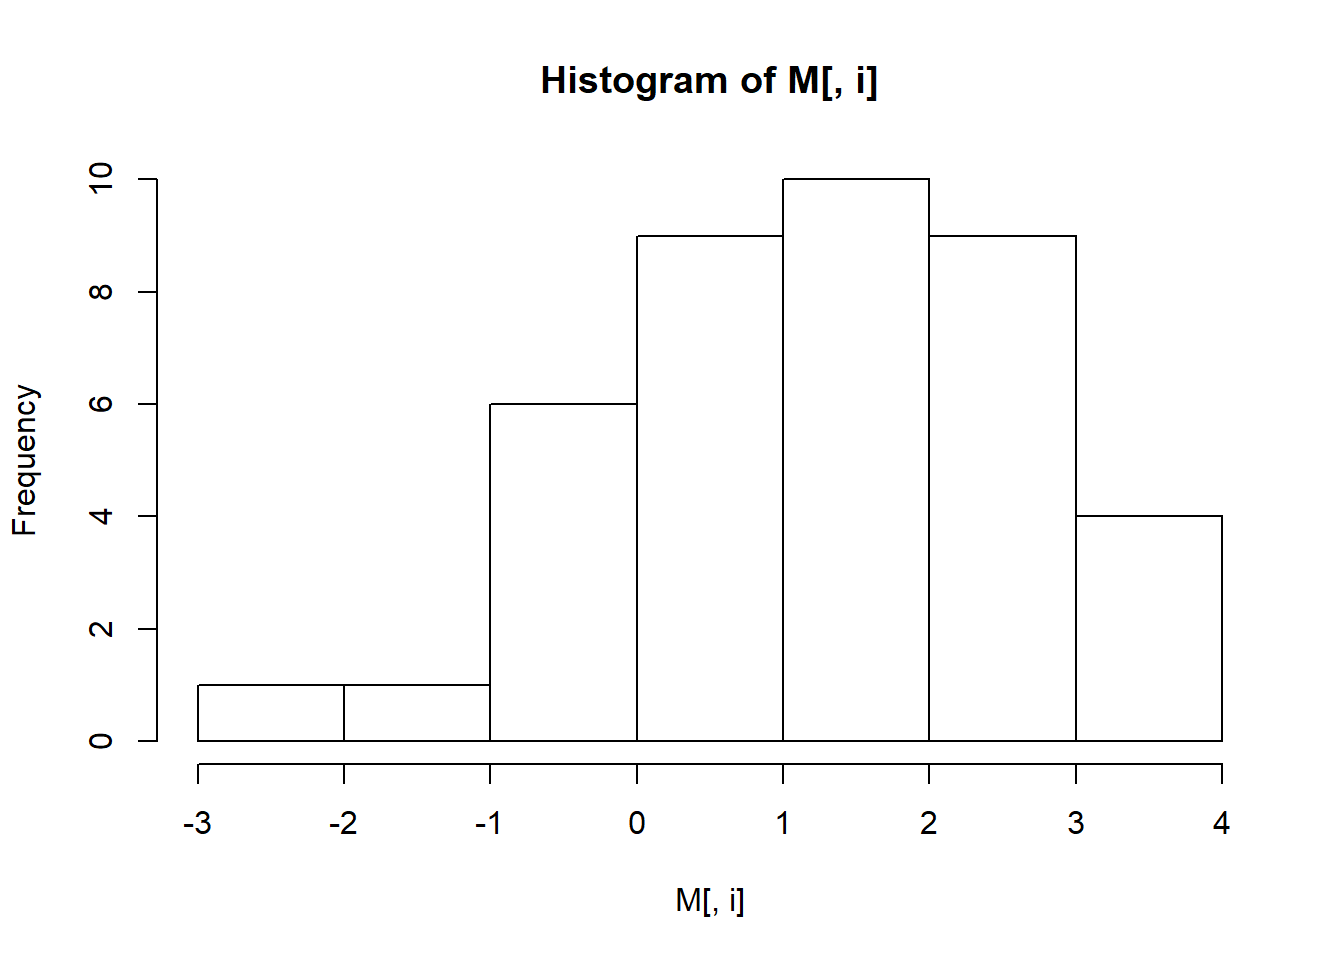
\includegraphics{plotandexplain_files/figure-latex/unnamed-chunk-3-27.pdf}
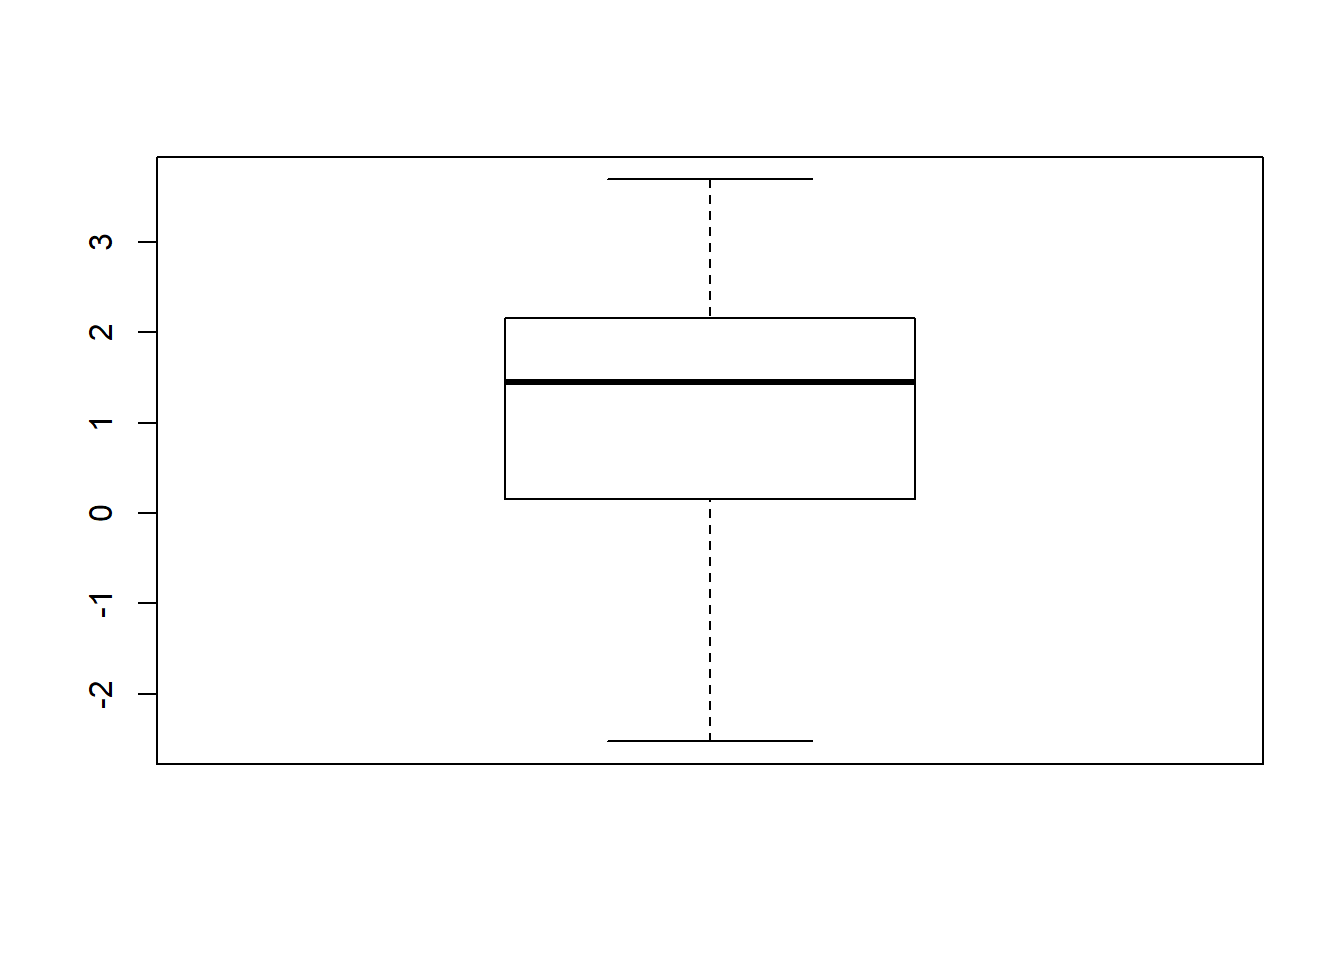
\includegraphics{plotandexplain_files/figure-latex/unnamed-chunk-3-28.pdf}
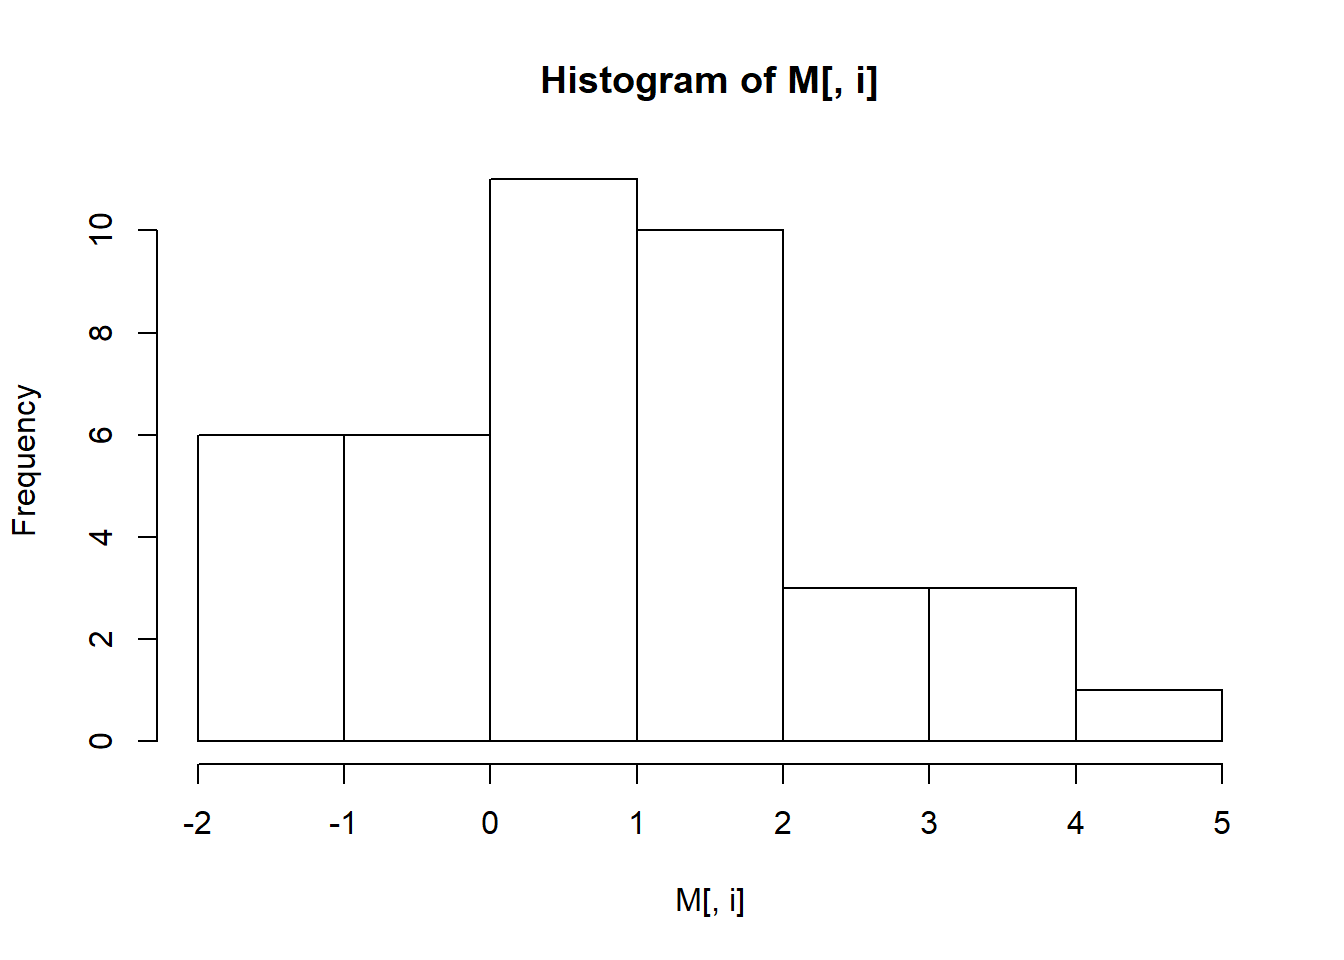
\includegraphics{plotandexplain_files/figure-latex/unnamed-chunk-3-29.pdf}
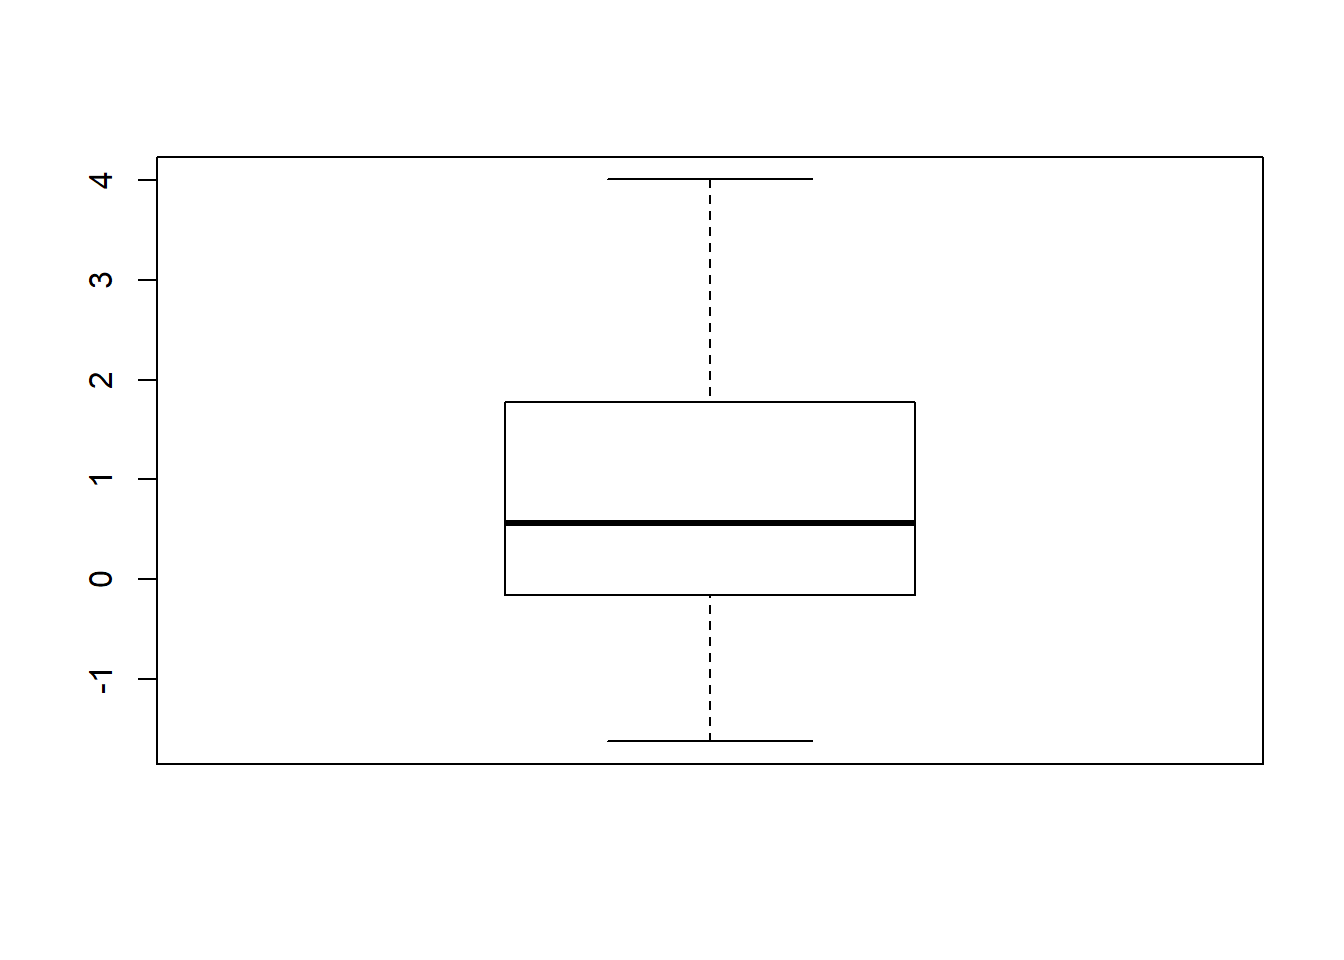
\includegraphics{plotandexplain_files/figure-latex/unnamed-chunk-3-30.pdf}
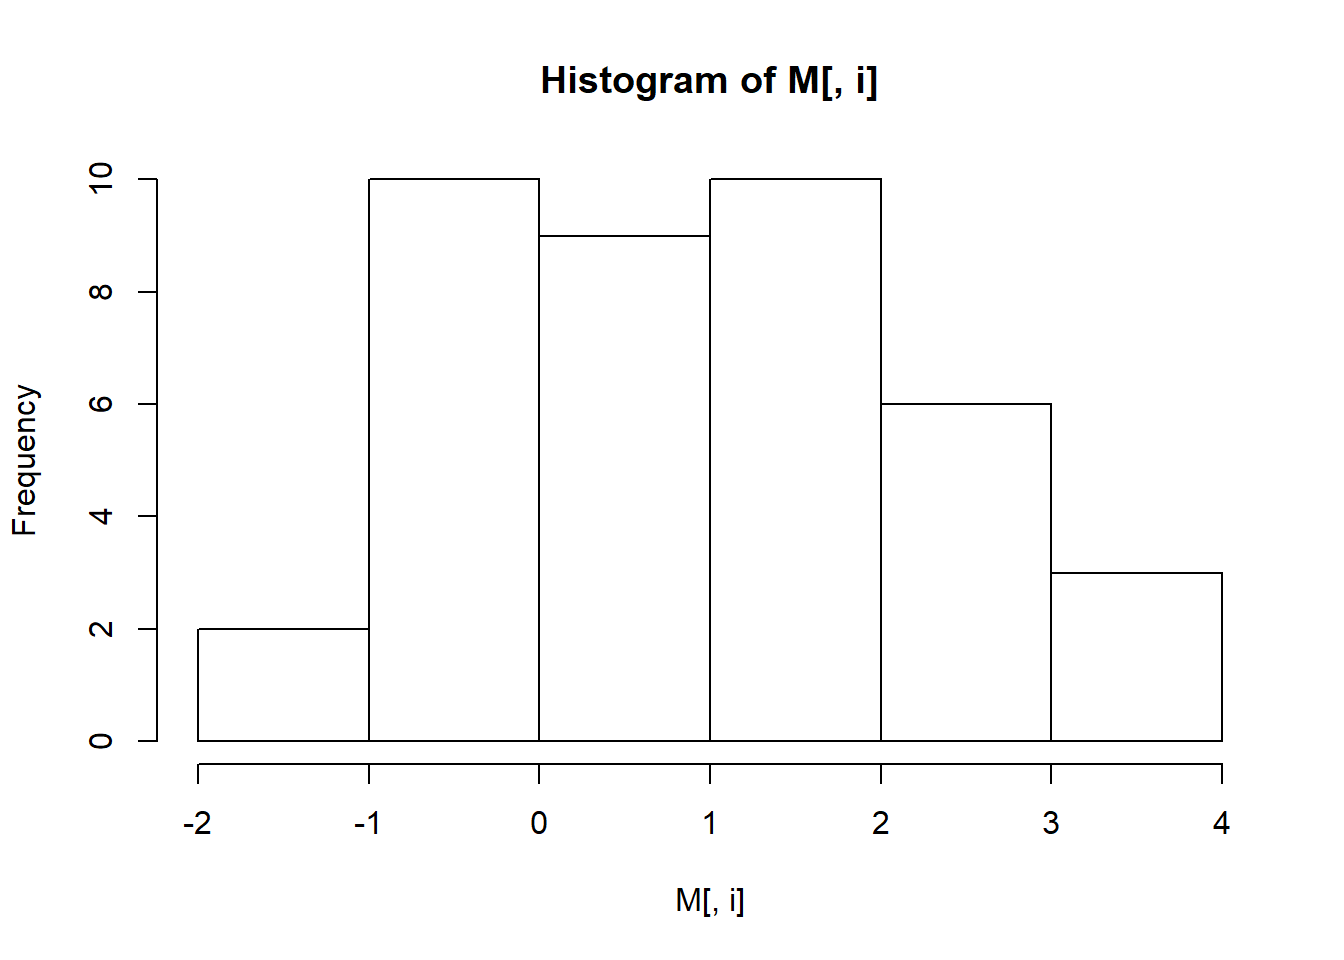
\includegraphics{plotandexplain_files/figure-latex/unnamed-chunk-3-31.pdf}
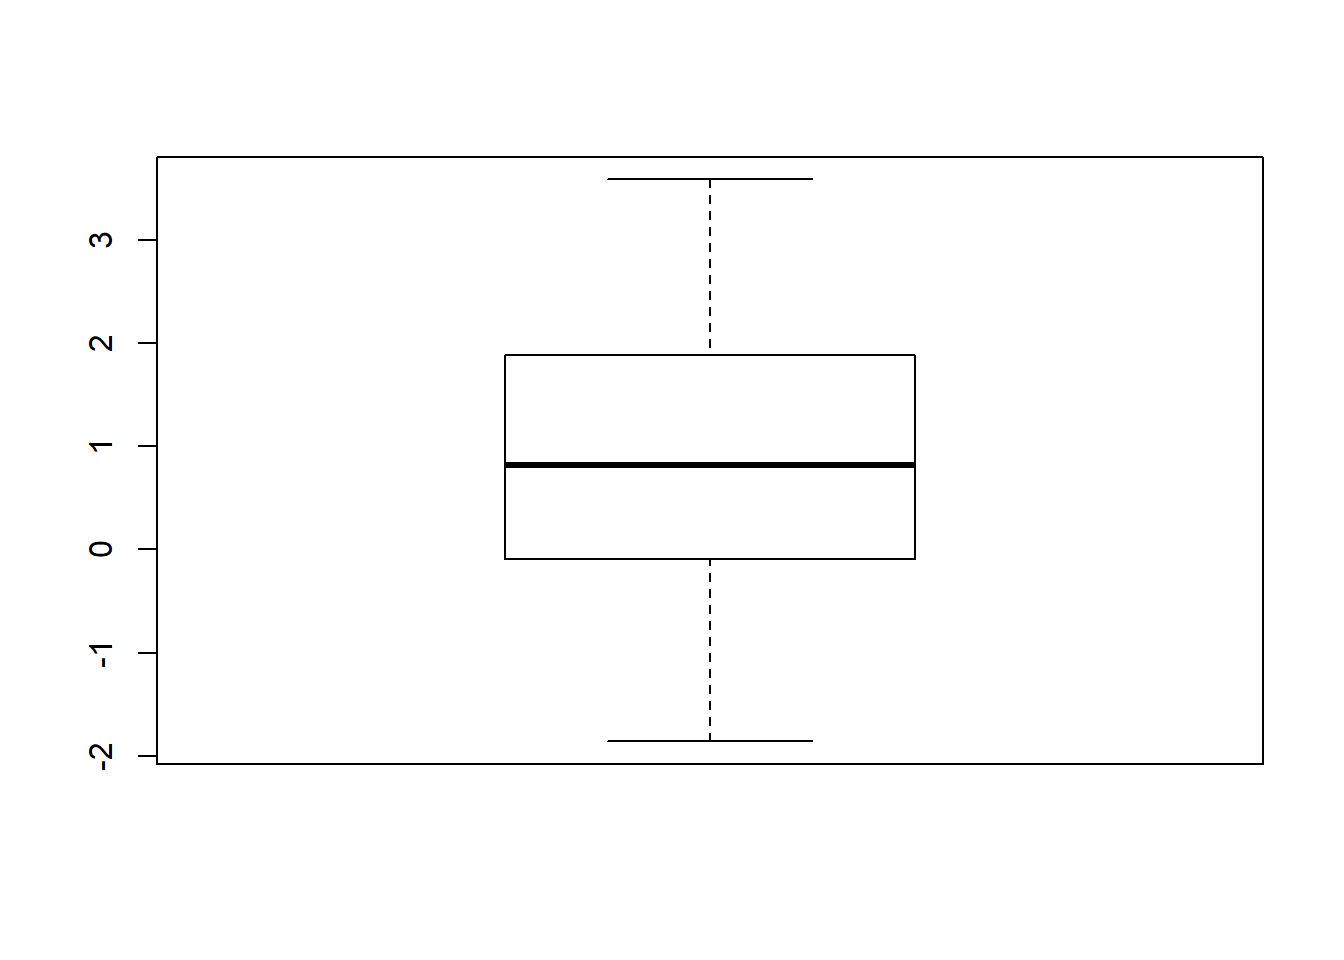
\includegraphics{plotandexplain_files/figure-latex/unnamed-chunk-3-32.pdf}
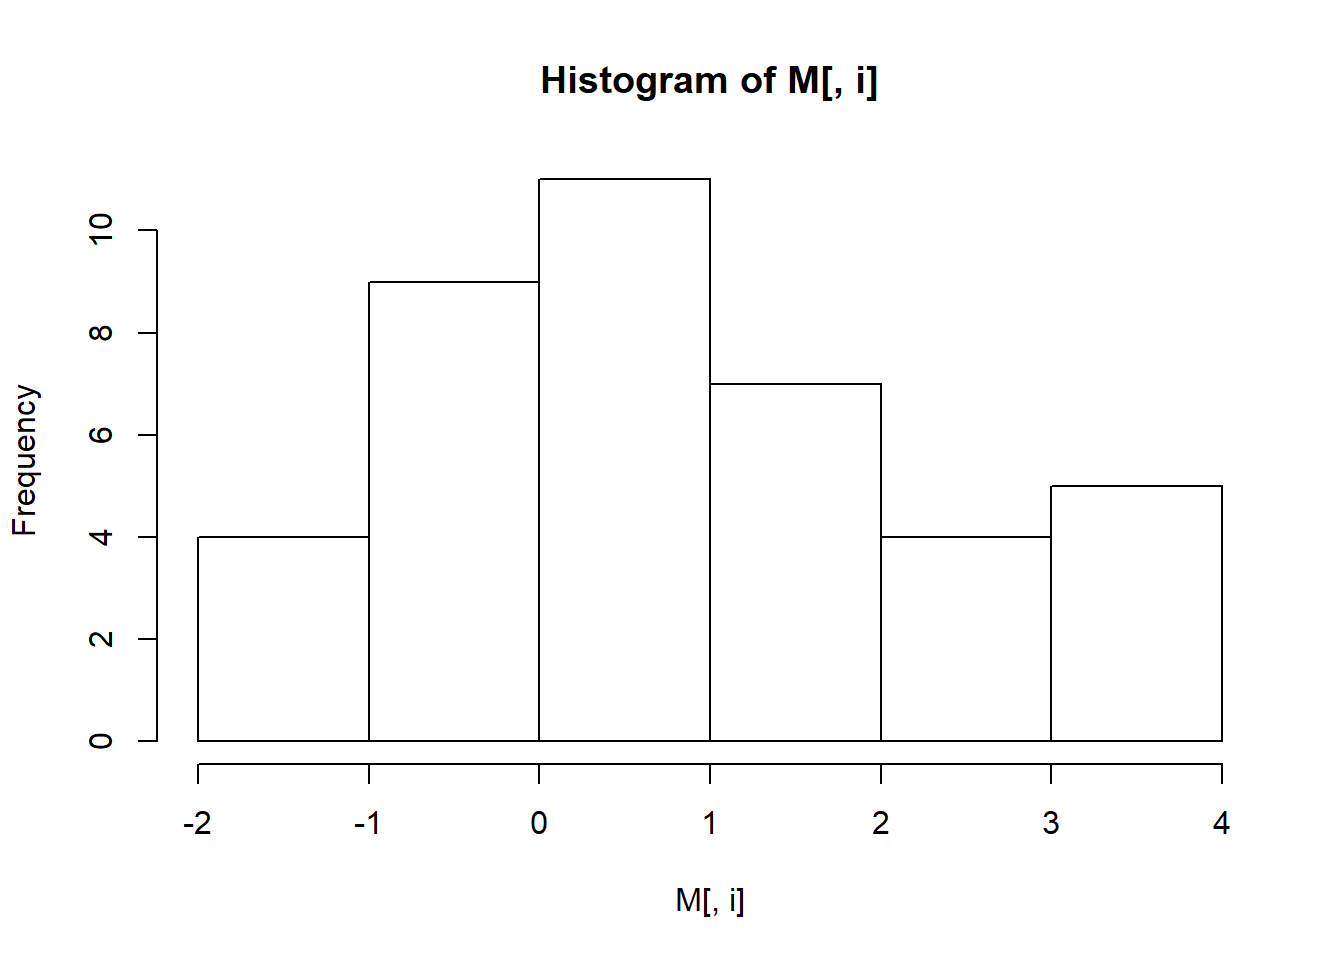
\includegraphics{plotandexplain_files/figure-latex/unnamed-chunk-3-33.pdf}
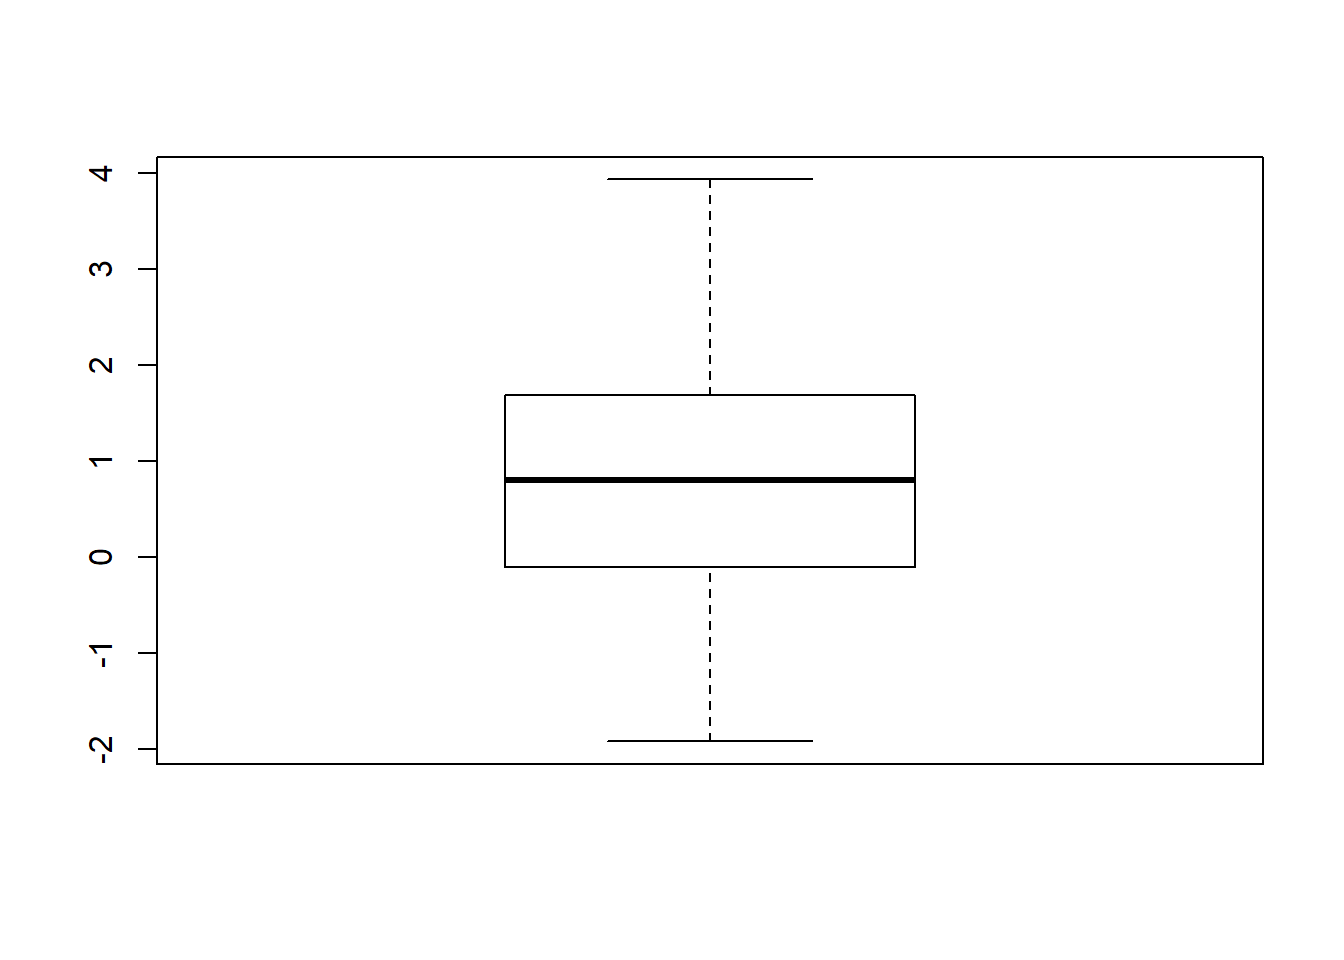
\includegraphics{plotandexplain_files/figure-latex/unnamed-chunk-3-34.pdf}
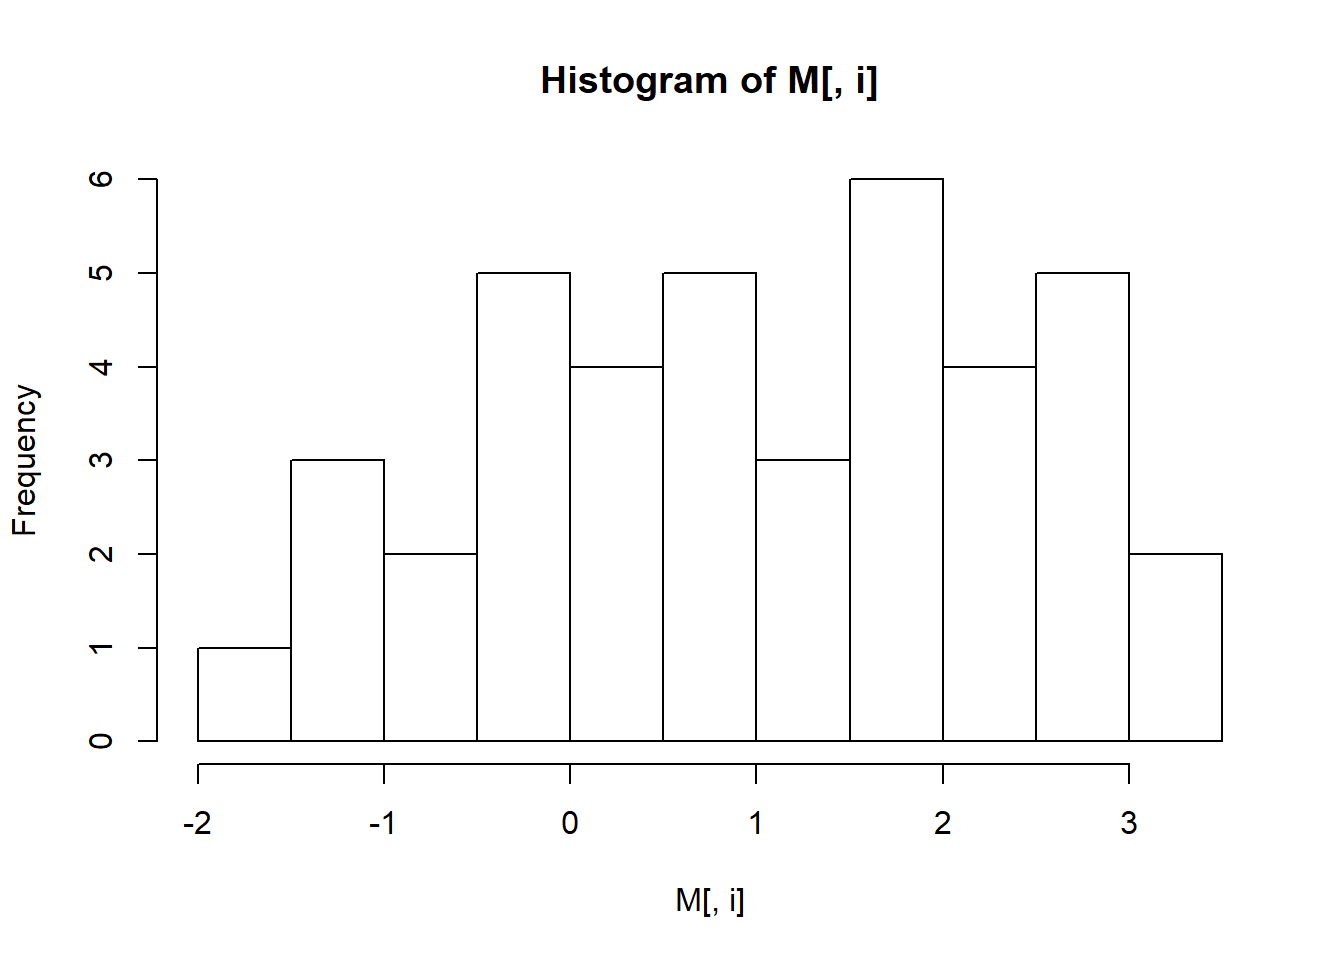
\includegraphics{plotandexplain_files/figure-latex/unnamed-chunk-3-35.pdf}
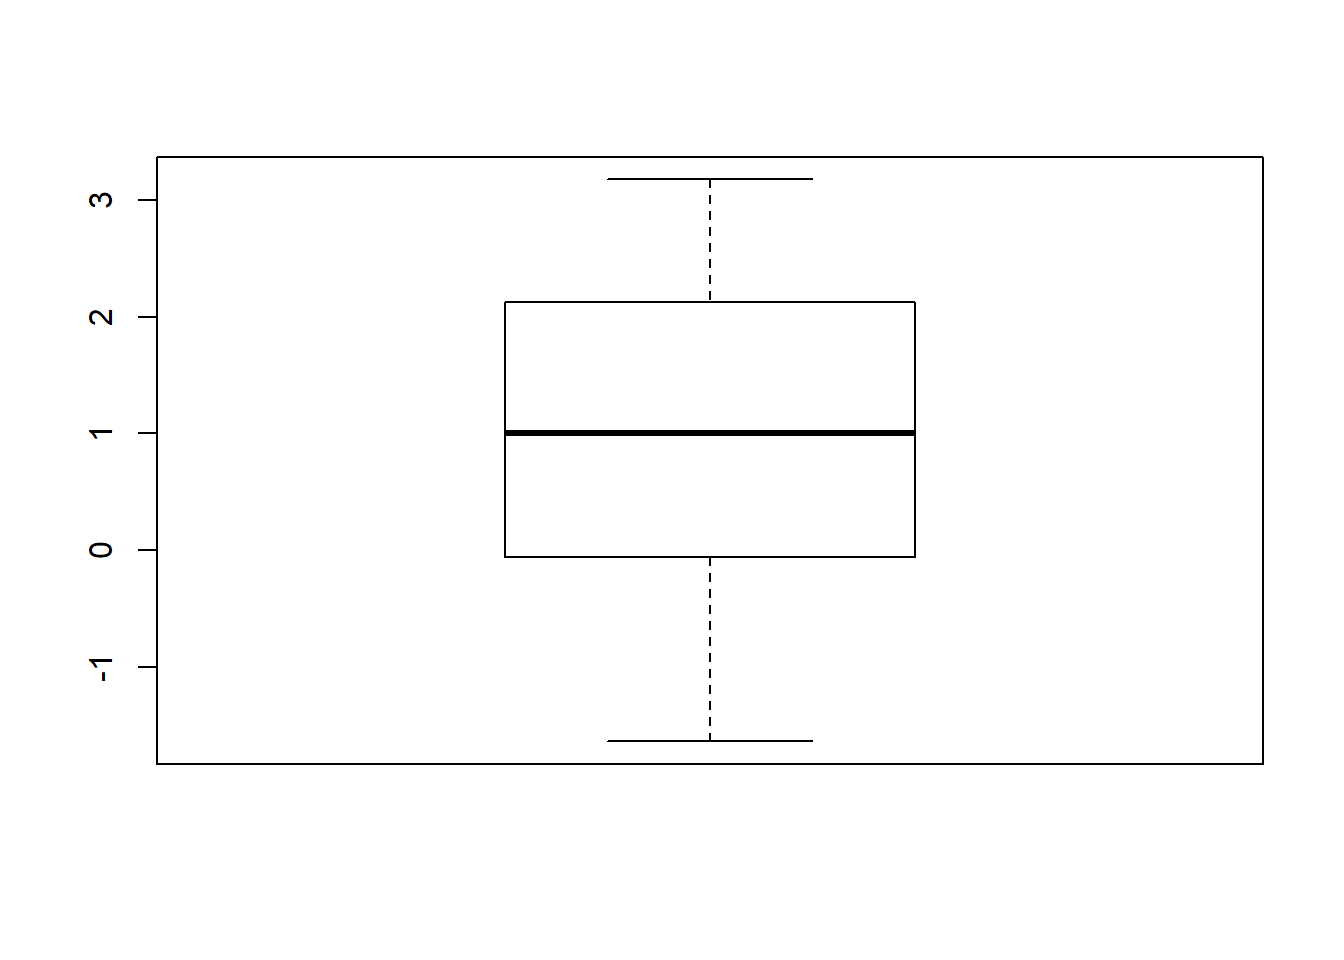
\includegraphics{plotandexplain_files/figure-latex/unnamed-chunk-3-36.pdf}
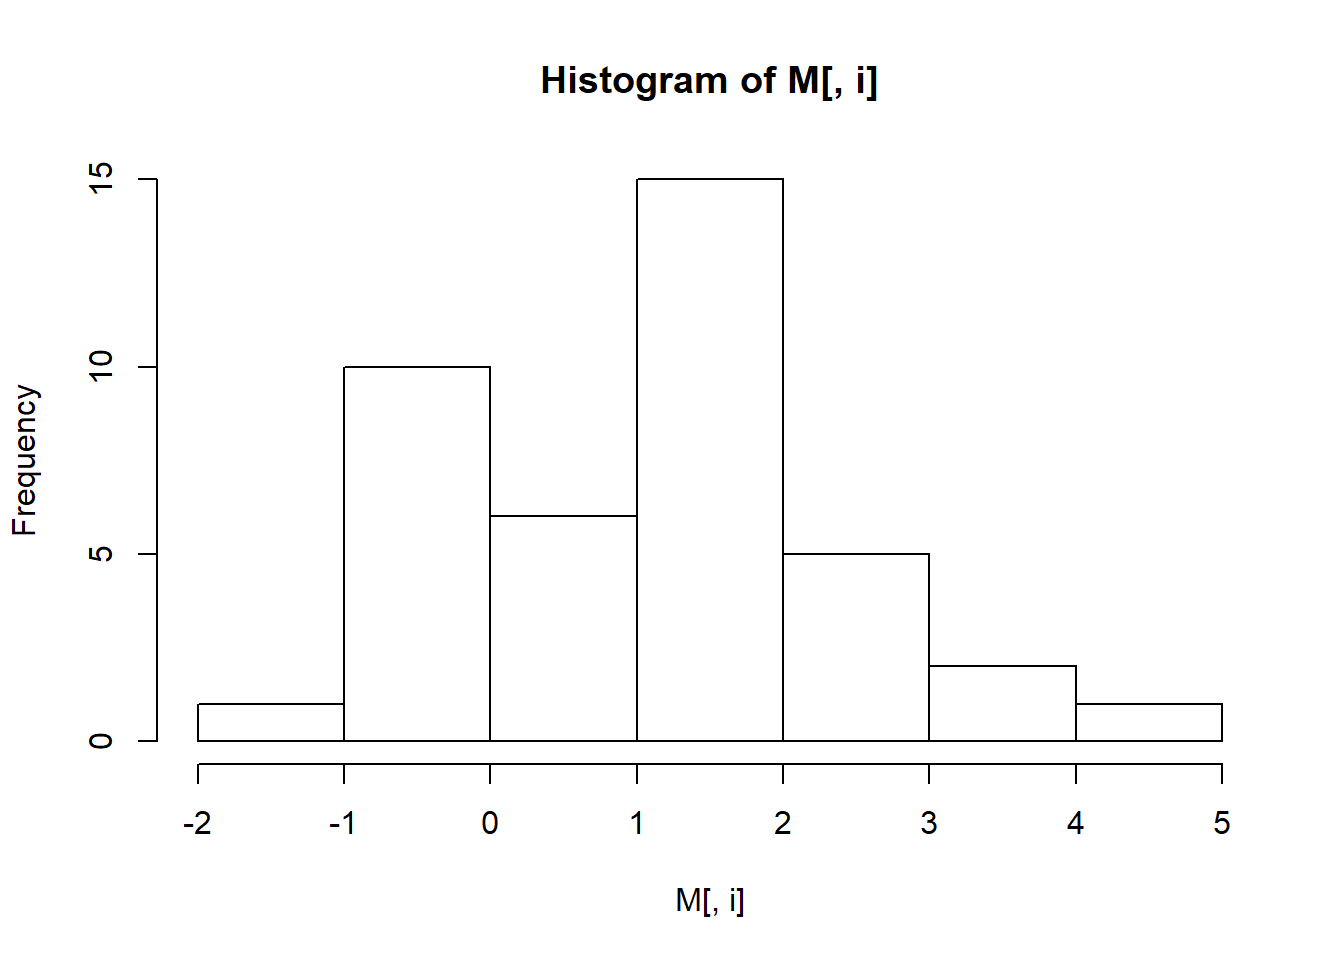
\includegraphics{plotandexplain_files/figure-latex/unnamed-chunk-3-37.pdf}
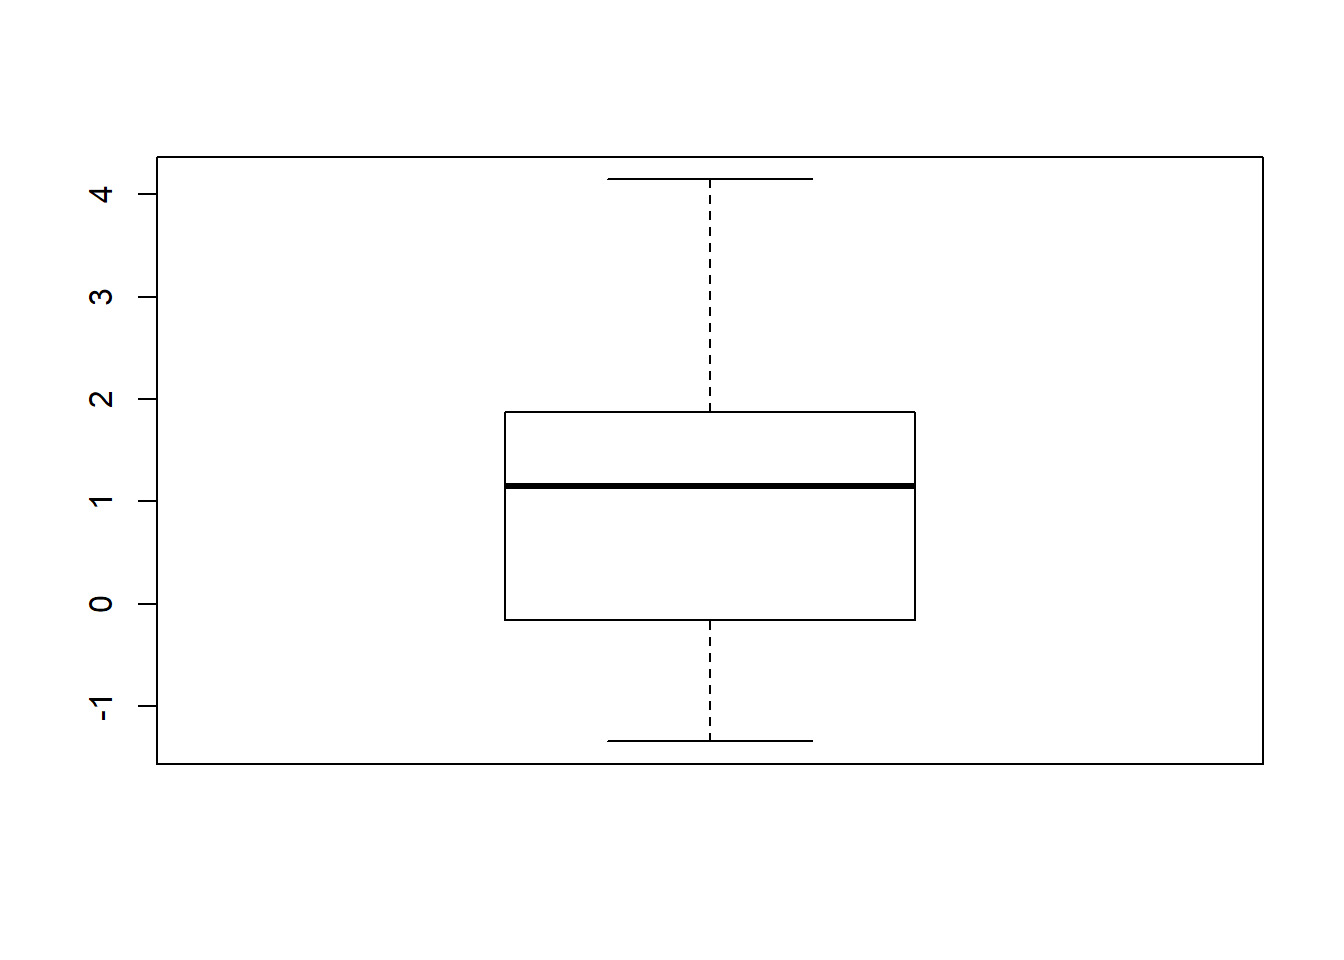
\includegraphics{plotandexplain_files/figure-latex/unnamed-chunk-3-38.pdf}
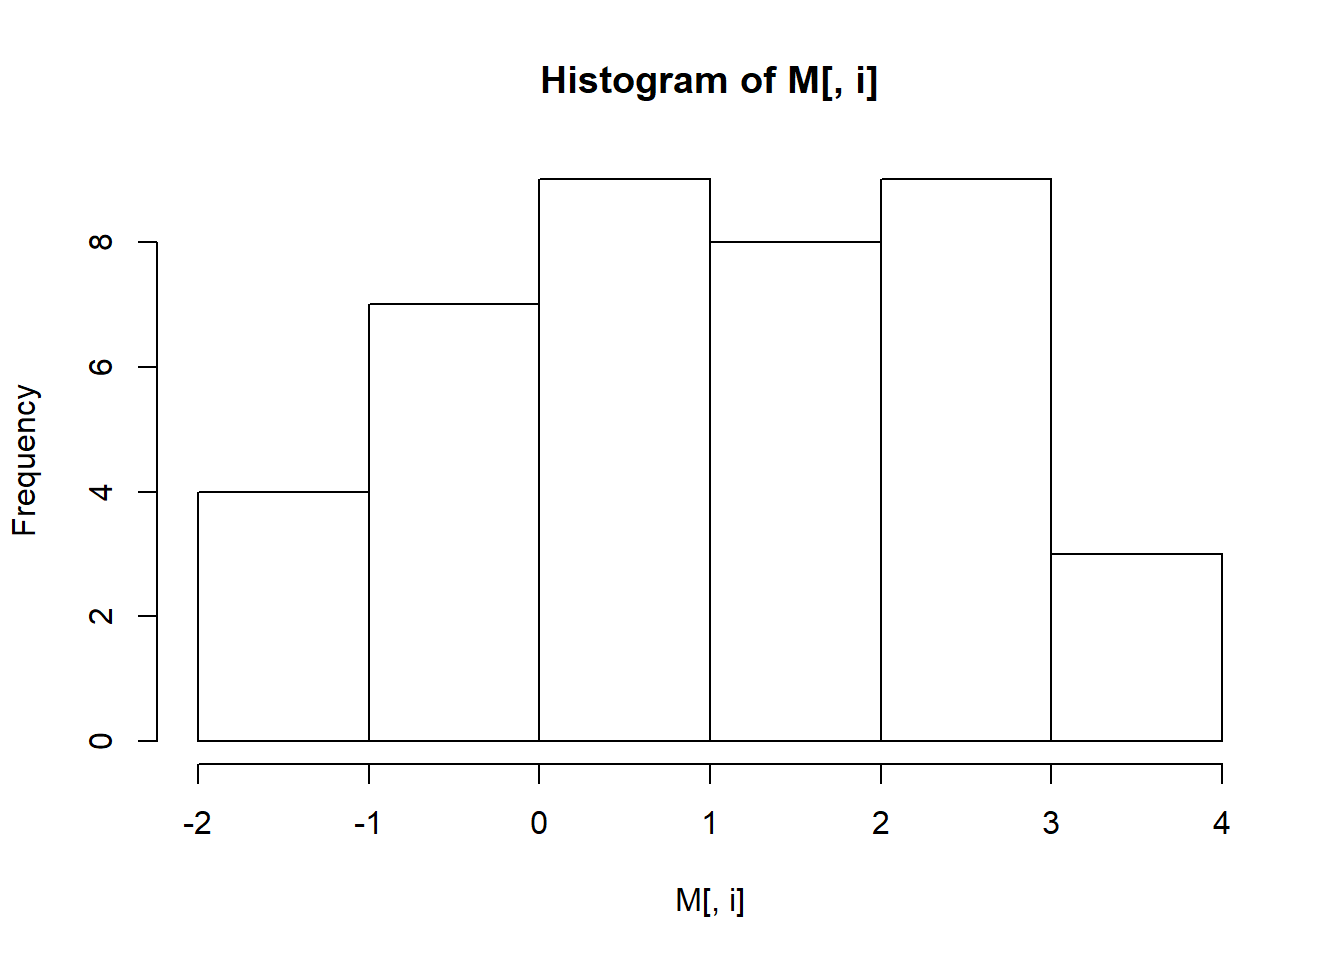
\includegraphics{plotandexplain_files/figure-latex/unnamed-chunk-3-39.pdf}
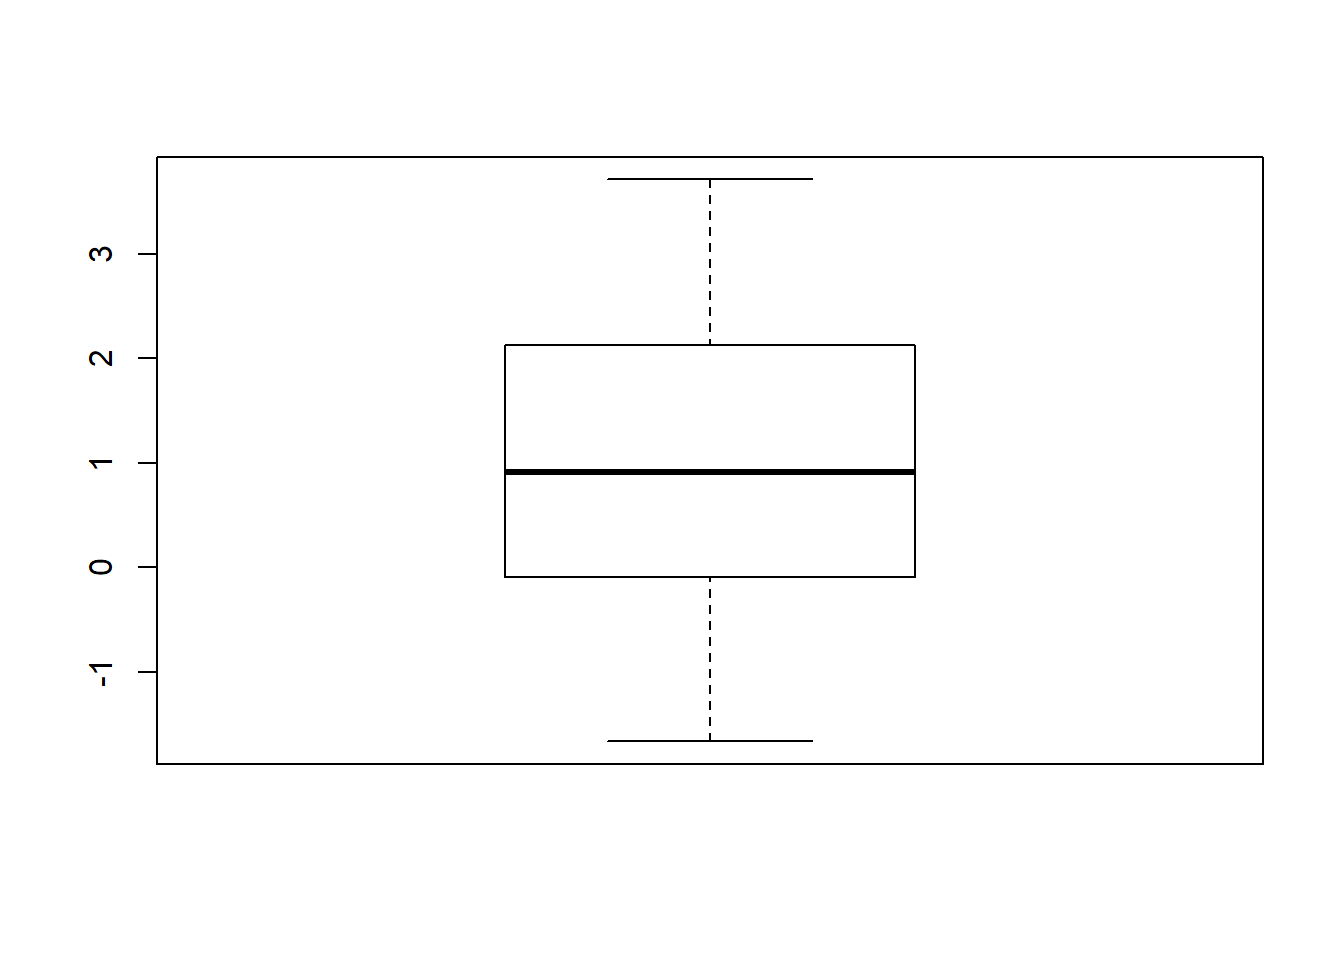
\includegraphics{plotandexplain_files/figure-latex/unnamed-chunk-3-40.pdf}
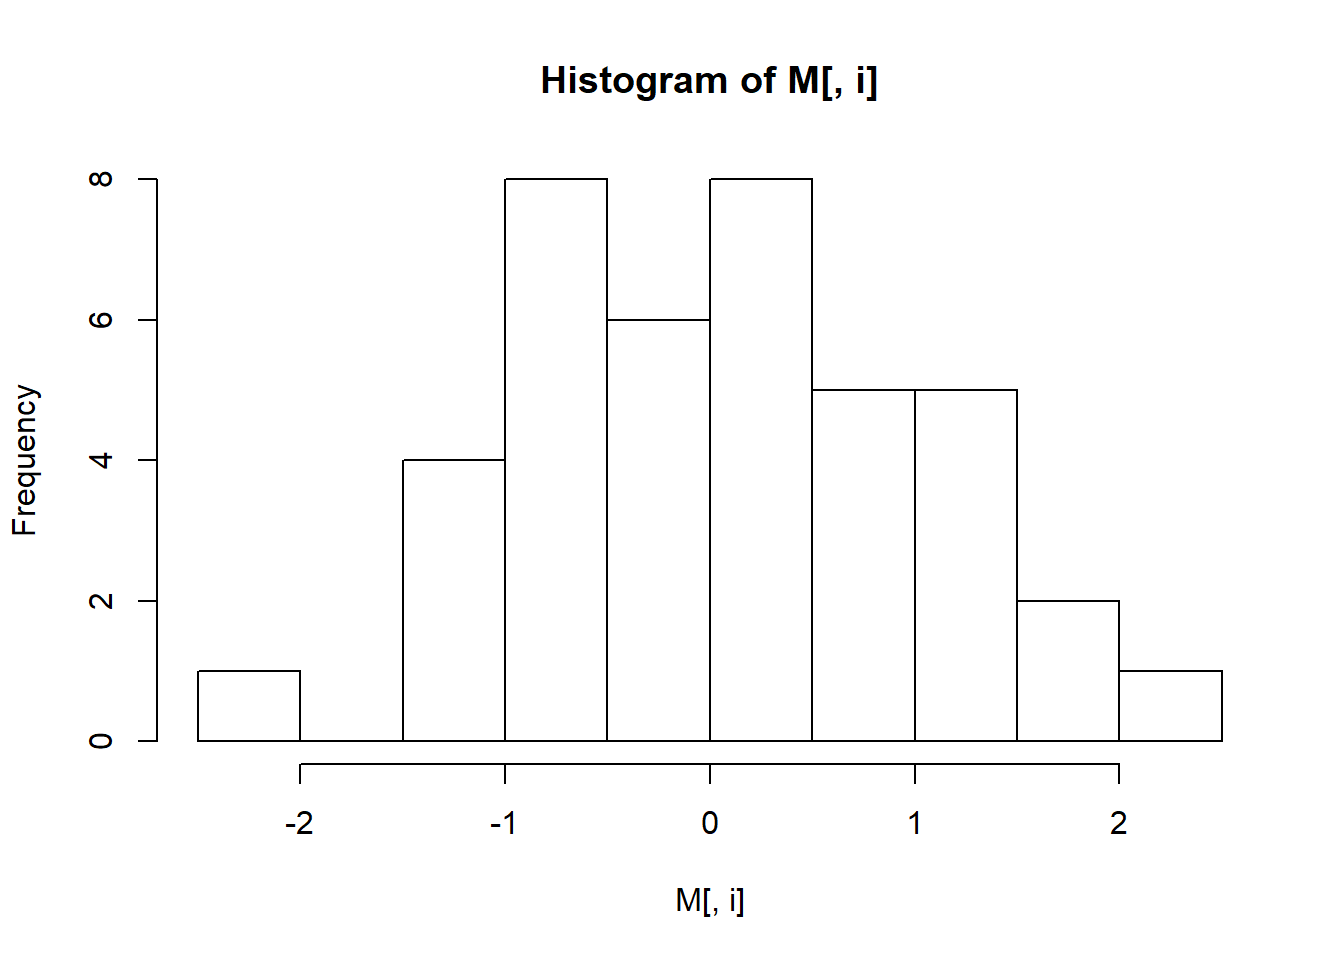
\includegraphics{plotandexplain_files/figure-latex/unnamed-chunk-3-41.pdf}
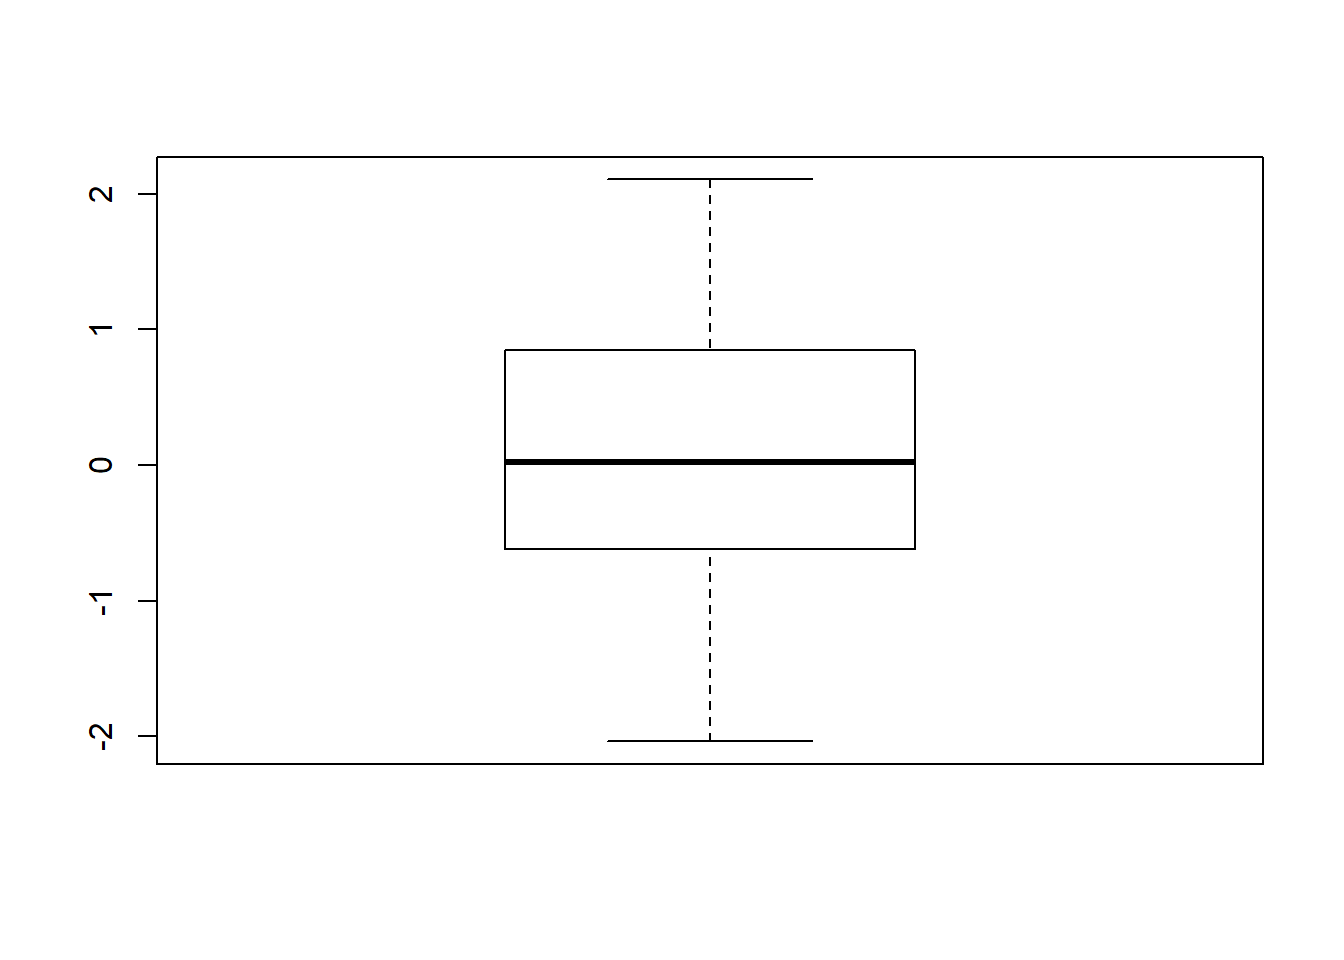
\includegraphics{plotandexplain_files/figure-latex/unnamed-chunk-3-42.pdf}
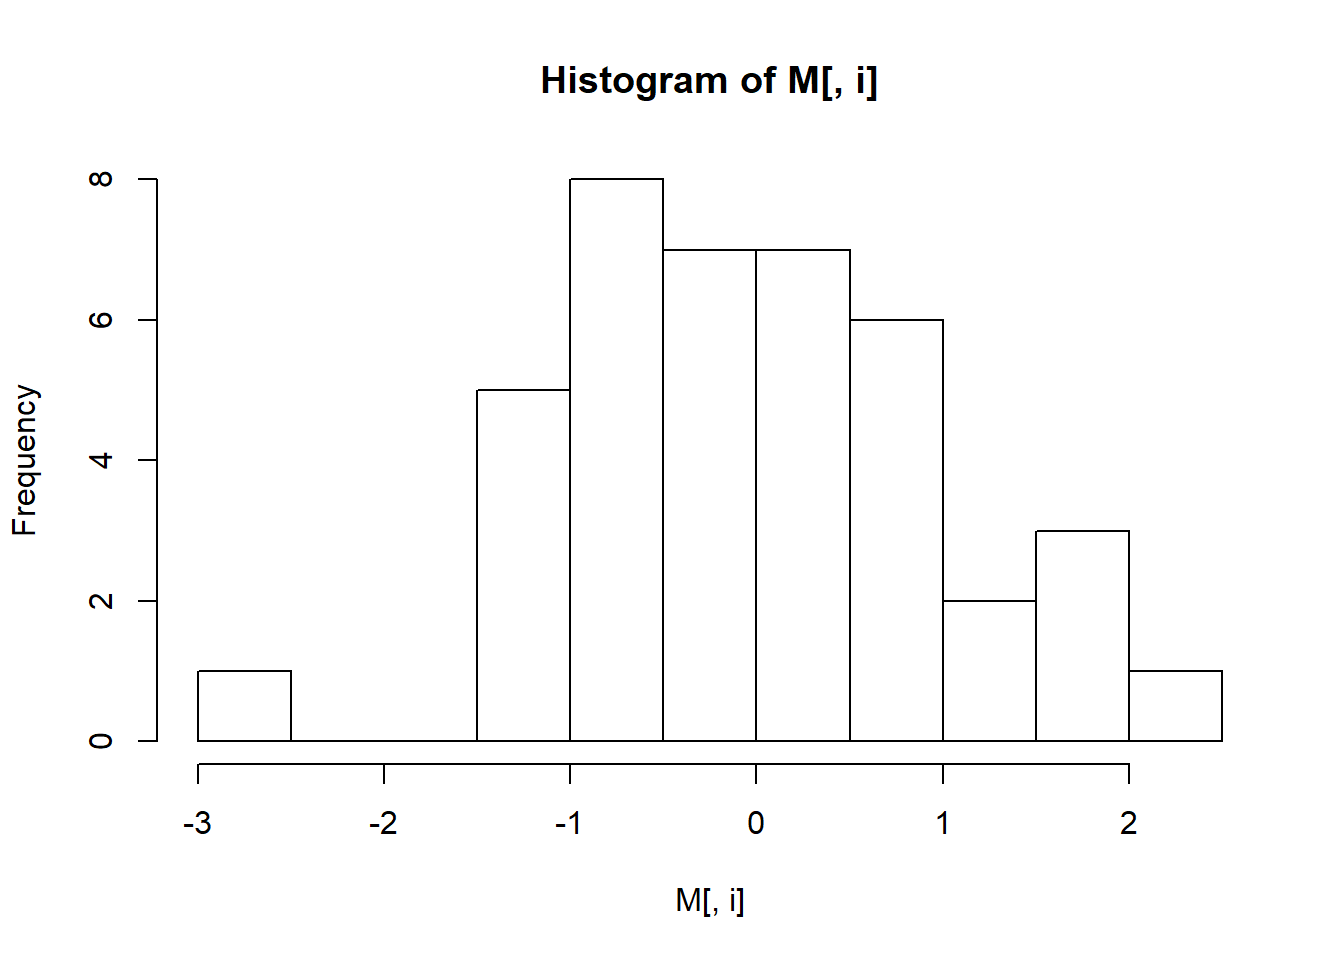
\includegraphics{plotandexplain_files/figure-latex/unnamed-chunk-3-43.pdf}
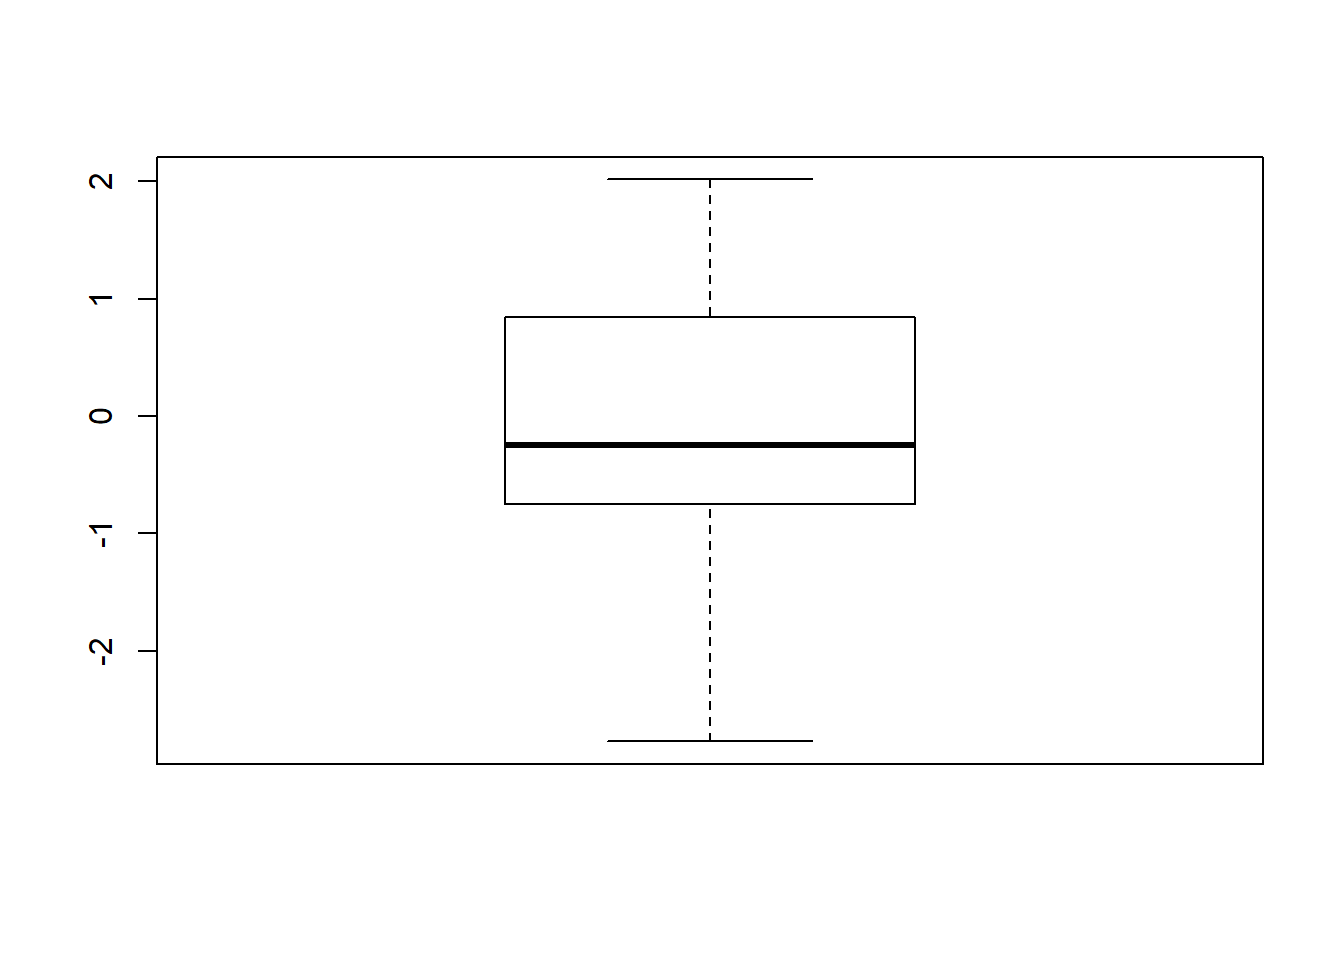
\includegraphics{plotandexplain_files/figure-latex/unnamed-chunk-3-44.pdf}
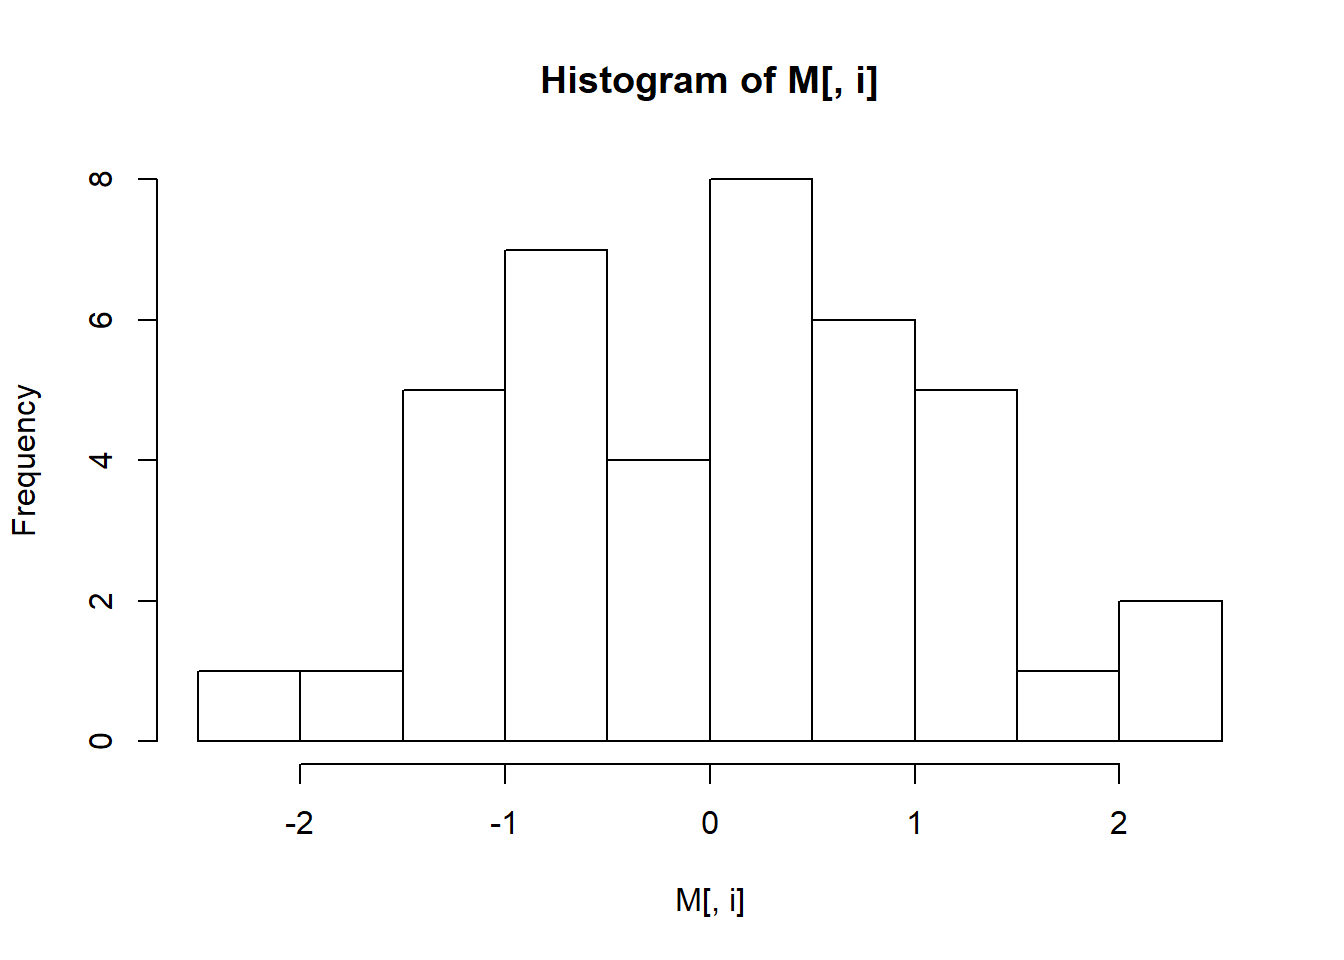
\includegraphics{plotandexplain_files/figure-latex/unnamed-chunk-3-45.pdf}
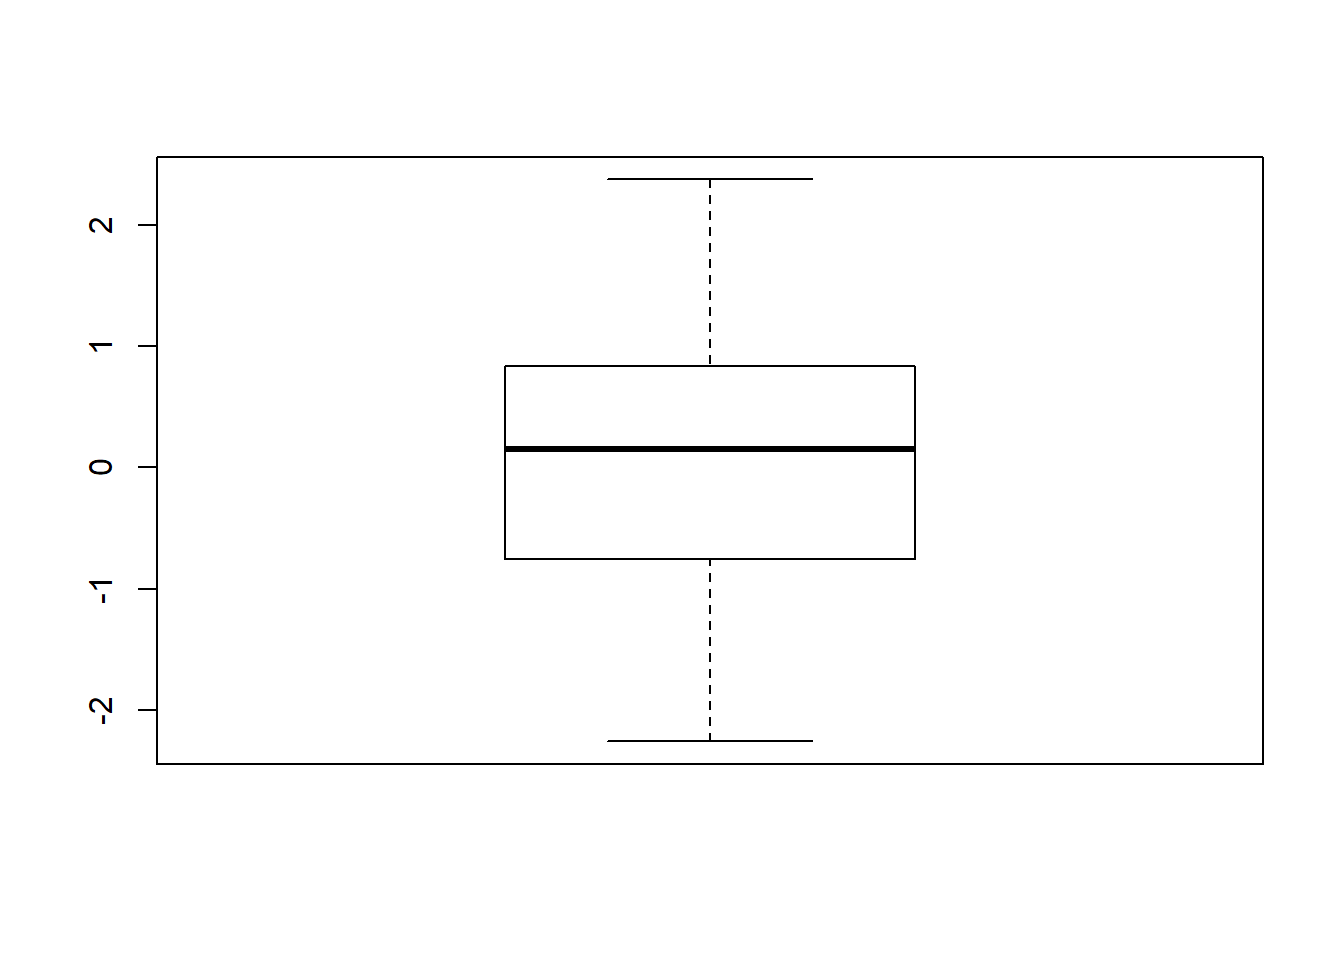
\includegraphics{plotandexplain_files/figure-latex/unnamed-chunk-3-46.pdf}
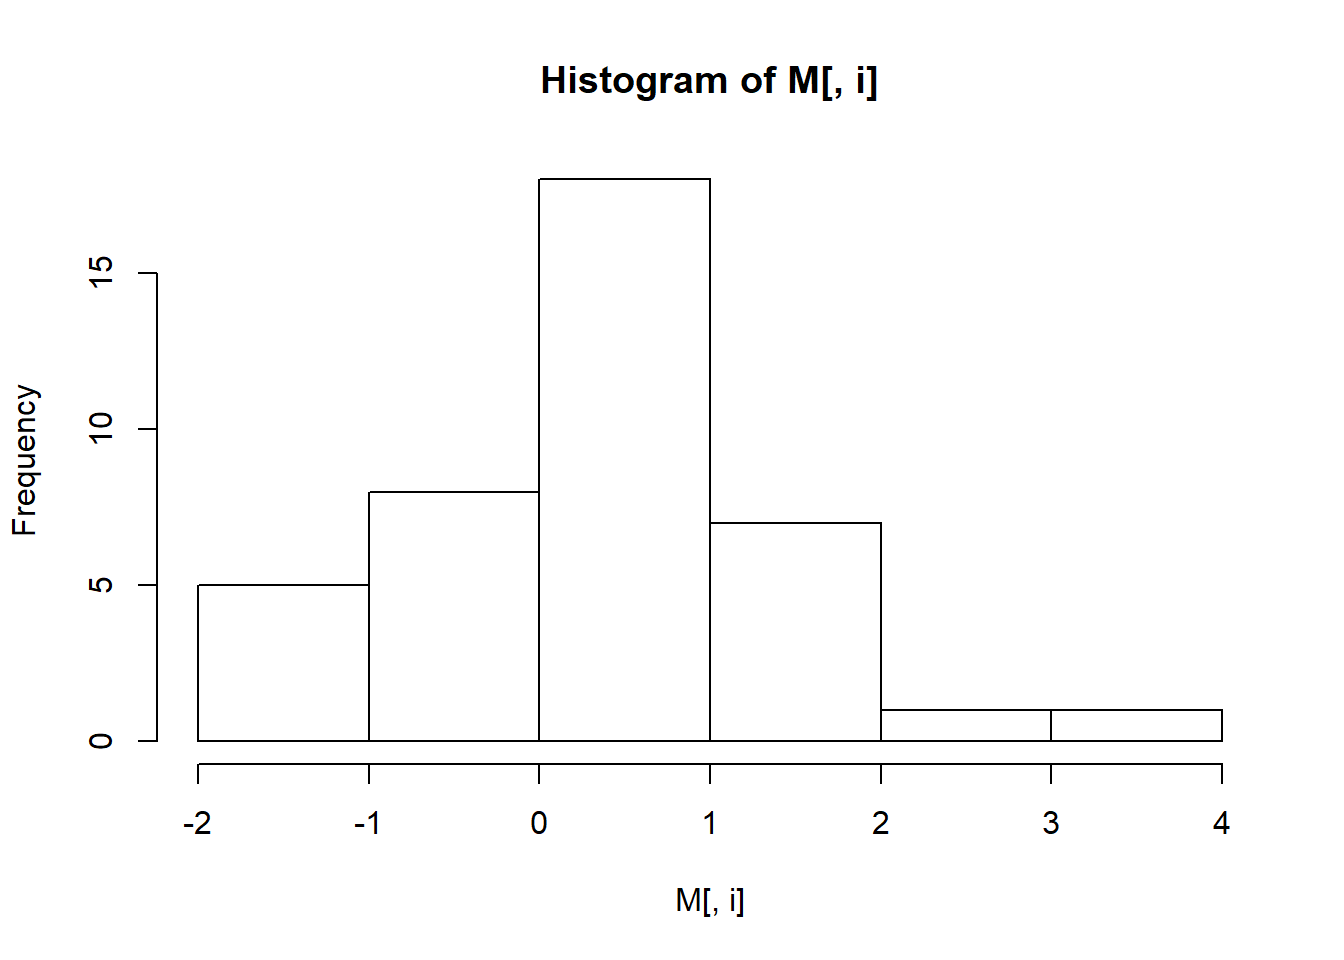
\includegraphics{plotandexplain_files/figure-latex/unnamed-chunk-3-47.pdf}
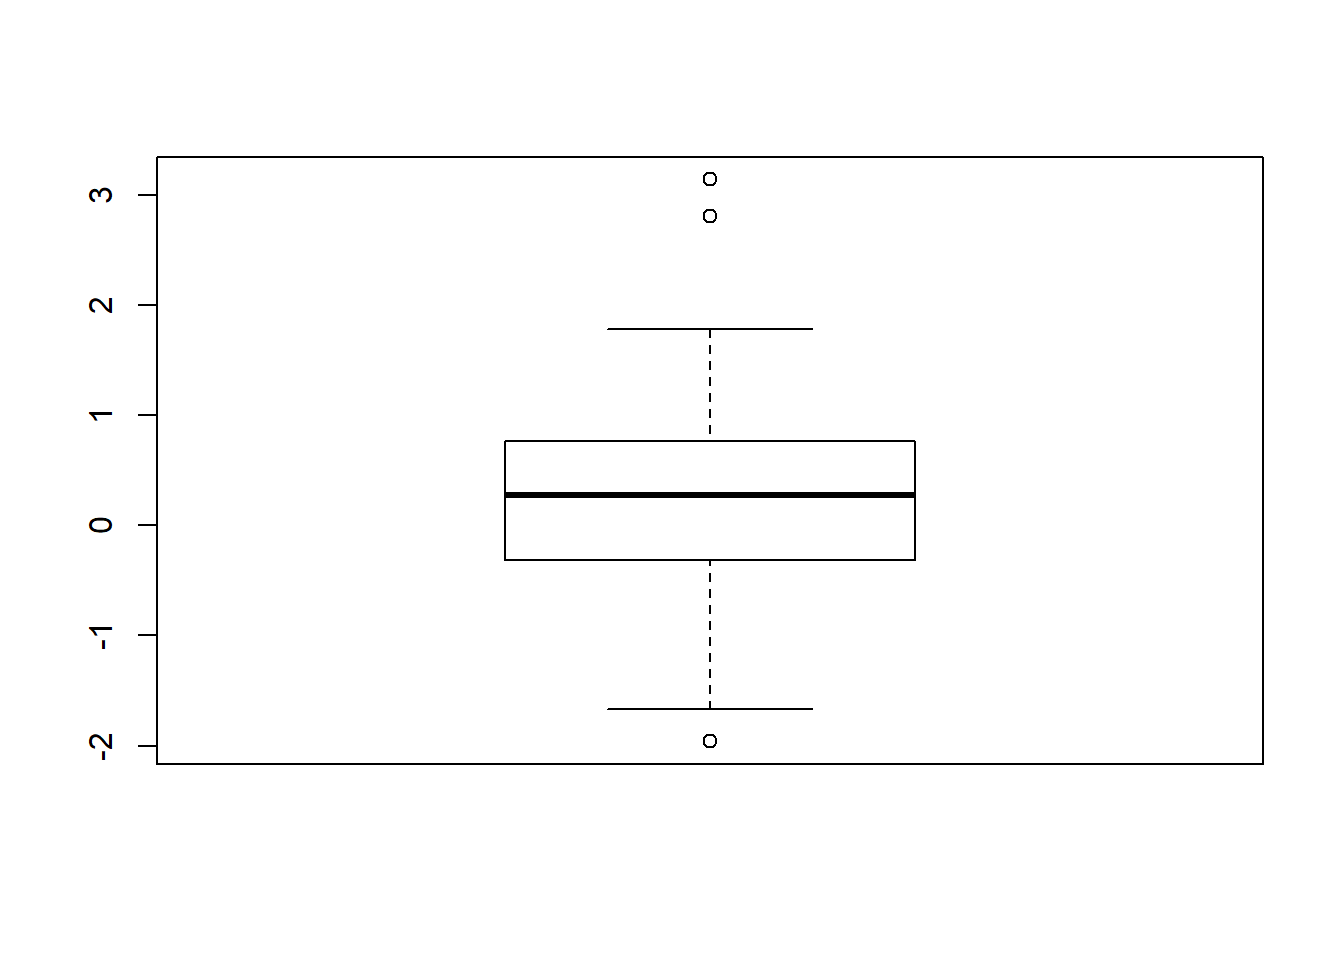
\includegraphics{plotandexplain_files/figure-latex/unnamed-chunk-3-48.pdf}
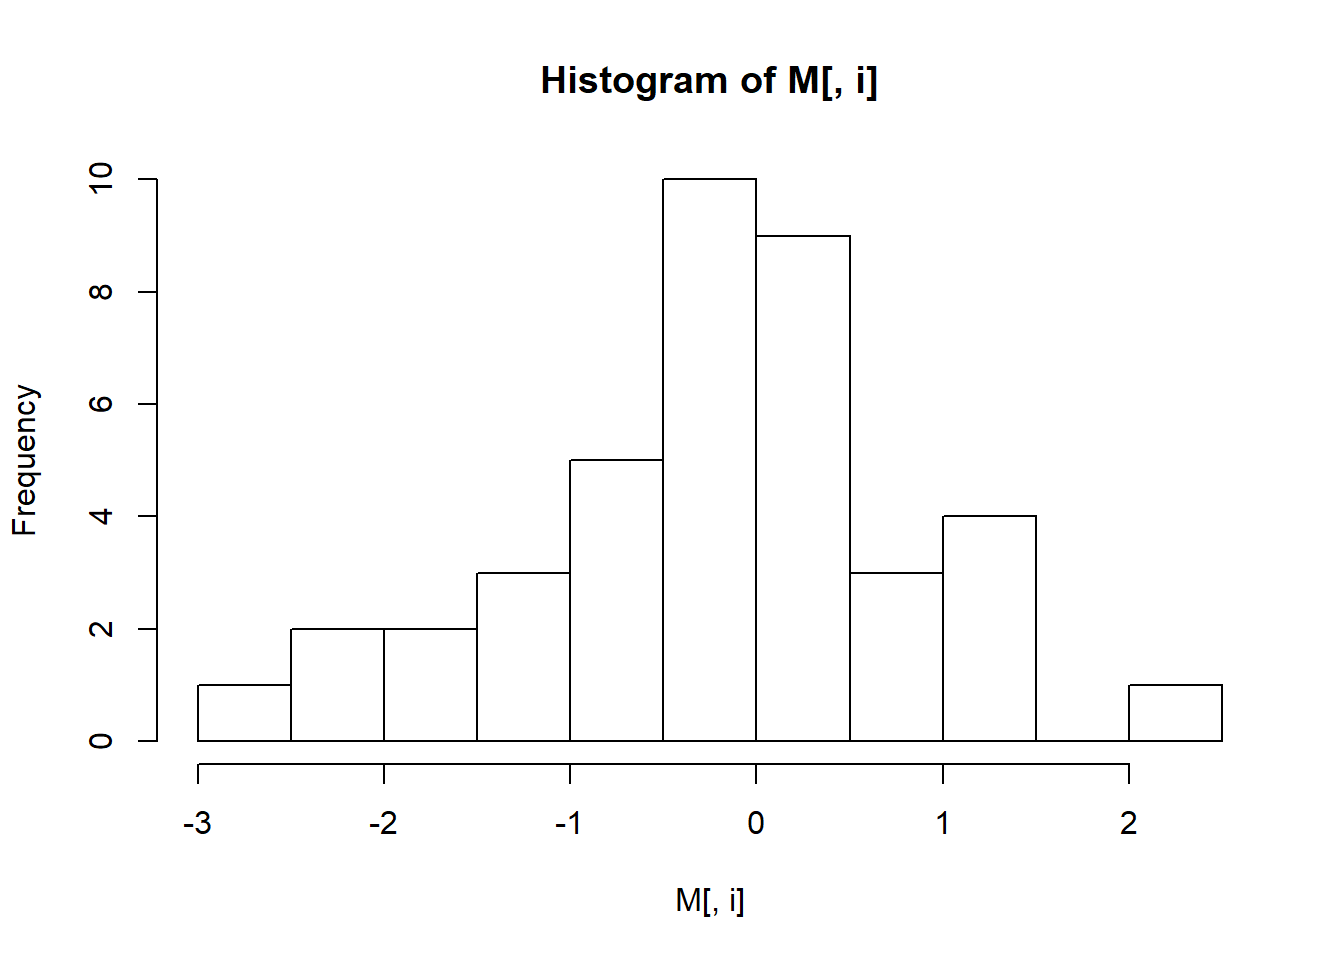
\includegraphics{plotandexplain_files/figure-latex/unnamed-chunk-3-49.pdf}
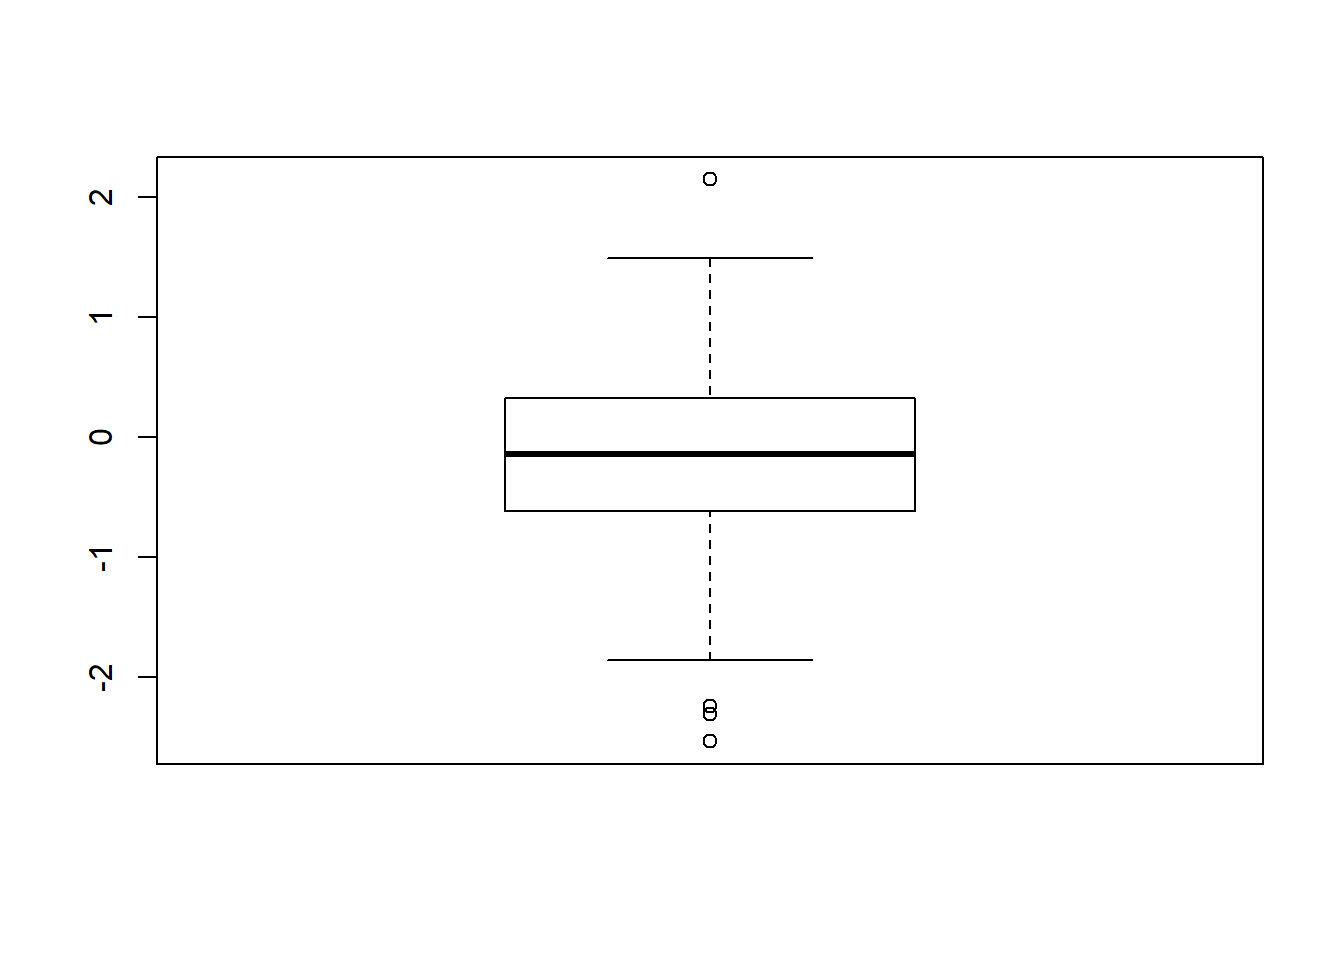
\includegraphics{plotandexplain_files/figure-latex/unnamed-chunk-3-50.pdf}
\includegraphics{plotandexplain_files/figure-latex/unnamed-chunk-3-51.pdf}
\includegraphics{plotandexplain_files/figure-latex/unnamed-chunk-3-52.pdf}
\includegraphics{plotandexplain_files/figure-latex/unnamed-chunk-3-53.pdf}
\includegraphics{plotandexplain_files/figure-latex/unnamed-chunk-3-54.pdf}
\includegraphics{plotandexplain_files/figure-latex/unnamed-chunk-3-55.pdf}
\includegraphics{plotandexplain_files/figure-latex/unnamed-chunk-3-56.pdf}
\includegraphics{plotandexplain_files/figure-latex/unnamed-chunk-3-57.pdf}
\includegraphics{plotandexplain_files/figure-latex/unnamed-chunk-3-58.pdf}
\includegraphics{plotandexplain_files/figure-latex/unnamed-chunk-3-59.pdf}
\includegraphics{plotandexplain_files/figure-latex/unnamed-chunk-3-60.pdf}
\includegraphics{plotandexplain_files/figure-latex/unnamed-chunk-3-61.pdf}
\includegraphics{plotandexplain_files/figure-latex/unnamed-chunk-3-62.pdf}
\includegraphics{plotandexplain_files/figure-latex/unnamed-chunk-3-63.pdf}
\includegraphics{plotandexplain_files/figure-latex/unnamed-chunk-3-64.pdf}
\includegraphics{plotandexplain_files/figure-latex/unnamed-chunk-3-65.pdf}
\includegraphics{plotandexplain_files/figure-latex/unnamed-chunk-3-66.pdf}
\includegraphics{plotandexplain_files/figure-latex/unnamed-chunk-3-67.pdf}
\includegraphics{plotandexplain_files/figure-latex/unnamed-chunk-3-68.pdf}
\includegraphics{plotandexplain_files/figure-latex/unnamed-chunk-3-69.pdf}
\includegraphics{plotandexplain_files/figure-latex/unnamed-chunk-3-70.pdf}
\includegraphics{plotandexplain_files/figure-latex/unnamed-chunk-3-71.pdf}
\includegraphics{plotandexplain_files/figure-latex/unnamed-chunk-3-72.pdf}
\includegraphics{plotandexplain_files/figure-latex/unnamed-chunk-3-73.pdf}
\includegraphics{plotandexplain_files/figure-latex/unnamed-chunk-3-74.pdf}
\includegraphics{plotandexplain_files/figure-latex/unnamed-chunk-3-75.pdf}
\includegraphics{plotandexplain_files/figure-latex/unnamed-chunk-3-76.pdf}
\includegraphics{plotandexplain_files/figure-latex/unnamed-chunk-3-77.pdf}
\includegraphics{plotandexplain_files/figure-latex/unnamed-chunk-3-78.pdf}
\includegraphics{plotandexplain_files/figure-latex/unnamed-chunk-3-79.pdf}
\includegraphics{plotandexplain_files/figure-latex/unnamed-chunk-3-80.pdf}

\begin{verbatim}
## [1] "# ------------------------ # Comparison of position # ------------------------ # "
## v 1  : 
##     mean :  0.007365834 
##    median :  0.03384706 
##    mode :  numeric 
##    Comparison between mean and median :  Not centred but no outliersNULL
## [1] "------------------------"
## v 2  : 
##     mean :  -0.02111068 
##    median :  -0.007093533 
##    mode :  numeric 
##    Comparison between mean and median :  Not centred but no outliersNULL
## [1] "------------------------"
## v 3  : 
##     mean :  -0.01193171 
##    median :  0.000556495 
##    mode :  numeric 
##    Comparison between mean and median :  Not centred but no outliersNULL
## [1] "------------------------"
## v 4  : 
##     mean :  -0.01082818 
##    median :  0.01622336 
##    mode :  numeric 
##    Comparison between mean and median :  Not centred but no outliersNULL
## [1] "------------------------"
## v 5  : 
##     mean :  -0.04640893 
##    median :  -0.04477948 
##    mode :  numeric 
##    Comparison between mean and median :  Not centred but no outliersNULL
## [1] "------------------------"
## v 6  : 
##     mean :  -0.04258523 
##    median :  -0.01222969 
##    mode :  numeric 
##    Comparison between mean and median :  Not centred but no outliersNULL
## [1] "------------------------"
## v 7  : 
##     mean :  0.03413923 
##    median :  0.03159751 
##    mode :  numeric 
##    Comparison between mean and median :  Outliers detectedNULL
## [1] "------------------------"
## v 8  : 
##     mean :  -0.0142744 
##    median :  -0.04938994 
##    mode :  numeric 
##    Comparison between mean and median :  Not centred but no outliersNULL
## [1] "------------------------"
## v 9  : 
##     mean :  0.02088063 
##    median :  0.01144227 
##    mode :  numeric 
##    Comparison between mean and median :  Not centred but no outliersNULL
## [1] "------------------------"
## v 10  : 
##     mean :  0.01155105 
##    median :  -0.02687963 
##    mode :  numeric 
##    Comparison between mean and median :  Not centred but no outliersNULL
## [1] "------------------------"
## v 11  : 
##     mean :  -0.03911398 
##    median :  -0.05368254 
##    mode :  numeric 
##    Comparison between mean and median :  Not centred but no outliersNULL
## [1] "------------------------"
## v 12  : 
##     mean :  -0.04666336 
##    median :  -0.06011508 
##    mode :  numeric 
##    Comparison between mean and median :  Not centred but no outliersNULL
## [1] "------------------------"
## v 13  : 
##     mean :  -0.0118976 
##    median :  0.01645455 
##    mode :  numeric 
##    Comparison between mean and median :  Not centred but no outliersNULL
## [1] "------------------------"
## v 14  : 
##     mean :  -0.009227084 
##    median :  0.000803635 
##    mode :  numeric 
##    Comparison between mean and median :  Not centred but no outliersNULL
## [1] "------------------------"
## v 15  : 
##     mean :  0.004714823 
##    median :  -0.002387027 
##    mode :  numeric 
##    Comparison between mean and median :  Not centred but no outliersNULL
## [1] "------------------------"
## v 16  : 
##     mean :  0.001554051 
##    median :  -0.006047873 
##    mode :  numeric 
##    Comparison between mean and median :  Not centred but no outliersNULL
## [1] "------------------------"
## v 17  : 
##     mean :  0.003121266 
##    median :  -0.000632543 
##    mode :  numeric 
##    Comparison between mean and median :  Not centred but no outliersNULL
## [1] "------------------------"
## v 18  : 
##     mean :  -0.04010893 
##    median :  -0.04960611 
##    mode :  numeric 
##    Comparison between mean and median :  Not centred but no outliersNULL
## [1] "------------------------"
## v 19  : 
##     mean :  -0.04072381 
##    median :  -0.005867516 
##    mode :  numeric 
##    Comparison between mean and median :  Not centred but no outliersNULL
## [1] "------------------------"
## v 20  : 
##     mean :  -0.01137595 
##    median :  -0.01469028 
##    mode :  numeric 
##    Comparison between mean and median :  Not centred but no outliersNULL
## [1] "------------------------"
## v 21  : 
##     mean :  0.221751 
##    median :  0.1183306 
##    mode :  numeric 
##    Comparison between mean and median :  Not centred but no outliersNULL
## [1] "------------------------"
## v 22  : 
##     mean :  0.1881155 
##    median :  0.09149527 
##    mode :  numeric 
##    Comparison between mean and median :  Not centred but no outliersNULL
## [1] "------------------------"
## v 23  : 
##     mean :  0.1947244 
##    median :  0.0929321 
##    mode :  numeric 
##    Comparison between mean and median :  Not centred but no outliersNULL
## [1] "------------------------"
## v 24  : 
##     mean :  0.2441216 
##    median :  0.225741 
##    mode :  numeric 
##    Comparison between mean and median :  Outliers detectedNULL
## [1] "------------------------"
## v 25  : 
##     mean :  0.2136634 
##    median :  0.1713661 
##    mode :  numeric 
##    Comparison between mean and median :  Outliers detectedNULL
## [1] "------------------------"
## v 26  : 
##     mean :  0.2665618 
##    median :  0.1899926 
##    mode :  numeric 
##    Comparison between mean and median :  Not centred but no outliersNULL
## [1] "------------------------"
## v 27  : 
##     mean :  0.257719 
##    median :  0.161339 
##    mode :  numeric 
##    Comparison between mean and median :  Not centred but no outliersNULL
## [1] "------------------------"
## v 28  : 
##     mean :  0.2319367 
##    median :  0.132211 
##    mode :  numeric 
##    Comparison between mean and median :  Not centred but no outliersNULL
## [1] "------------------------"
## v 29  : 
##     mean :  0.2290427 
##    median :  0.1897611 
##    mode :  numeric 
##    Comparison between mean and median :  Outliers detectedNULL
## [1] "------------------------"
## v 30  : 
##     mean :  0.207009 
##    median :  0.168409 
##    mode :  numeric 
##    Comparison between mean and median :  Outliers detectedNULL
## [1] "------------------------"
## v 31  : 
##     mean :  0.190125 
##    median :  0.1179475 
##    mode :  numeric 
##    Comparison between mean and median :  Not centred but no outliersNULL
## [1] "------------------------"
## v 32  : 
##     mean :  0.2587154 
##    median :  0.1892092 
##    mode :  numeric 
##    Comparison between mean and median :  Not centred but no outliersNULL
## [1] "------------------------"
## v 33  : 
##     mean :  0.2212844 
##    median :  0.1409739 
##    mode :  numeric 
##    Comparison between mean and median :  Not centred but no outliersNULL
## [1] "------------------------"
## v 34  : 
##     mean :  0.2107588 
##    median :  0.1528187 
##    mode :  numeric 
##    Comparison between mean and median :  Not centred but no outliersNULL
## [1] "------------------------"
## v 35  : 
##     mean :  0.1739681 
##    median :  0.1083145 
##    mode :  numeric 
##    Comparison between mean and median :  Not centred but no outliersNULL
## [1] "------------------------"
## v 36  : 
##     mean :  0.2266386 
##    median :  0.1041938 
##    mode :  numeric 
##    Comparison between mean and median :  Not centred but no outliersNULL
## [1] "------------------------"
## v 37  : 
##     mean :  0.2812307 
##    median :  0.2204154 
##    mode :  numeric 
##    Comparison between mean and median :  Outliers detectedNULL
## [1] "------------------------"
## v 38  : 
##     mean :  0.2254397 
##    median :  0.1616018 
##    mode :  numeric 
##    Comparison between mean and median :  Not centred but no outliersNULL
## [1] "------------------------"
## v 39  : 
##     mean :  0.2206724 
##    median :  0.1177003 
##    mode :  numeric 
##    Comparison between mean and median :  Not centred but no outliersNULL
## [1] "------------------------"
## v 40  : 
##     mean :  0.2802789 
##    median :  0.2041018 
##    mode :  numeric 
##    Comparison between mean and median :  Not centred but no outliersNULL
## [1] "------------------------"
## [1] "# ------------------------ # Comparison of dispersion # ------------------------ # "
## v 1  : 
##     standart deviation :  0.9981043 
##    scope (outliers can affect) :  0.462971 
##    interquantile deviation :  -0.00506715NULL
## [1] "------------------------"
## v 2  : 
##     standart deviation :  0.9975872 
##    scope (outliers can affect) :  -0.15649 
##    interquantile deviation :  -0.04328585NULL
## [1] "------------------------"
## v 3  : 
##     standart deviation :  1.008454 
##    scope (outliers can affect) :  -0.068637 
##    interquantile deviation :  -0.0936771NULL
## [1] "------------------------"
## v 4  : 
##     standart deviation :  1.01263 
##    scope (outliers can affect) :  0.156605 
##    interquantile deviation :  -0.03306125NULL
## [1] "------------------------"
## v 5  : 
##     standart deviation :  1.01681 
##    scope (outliers can affect) :  -0.099949 
##    interquantile deviation :  -0.07355355NULL
## [1] "------------------------"
## v 6  : 
##     standart deviation :  0.9906852 
##    scope (outliers can affect) :  0.21567 
##    interquantile deviation :  -0.08430005NULL
## [1] "------------------------"
## v 7  : 
##     standart deviation :  1.022581 
##    scope (outliers can affect) :  1.145586 
##    interquantile deviation :  0.0451339NULL
## [1] "------------------------"
## v 8  : 
##     standart deviation :  0.9996908 
##    scope (outliers can affect) :  -0.273623 
##    interquantile deviation :  -0.0232934NULL
## [1] "------------------------"
## v 9  : 
##     standart deviation :  0.9826407 
##    scope (outliers can affect) :  -0.082523 
##    interquantile deviation :  0.0352292NULL
## [1] "------------------------"
## v 10  : 
##     standart deviation :  1.002846 
##    scope (outliers can affect) :  0.976503 
##    interquantile deviation :  -0.0069748NULL
## [1] "------------------------"
## v 11  : 
##     standart deviation :  0.9924397 
##    scope (outliers can affect) :  -0.260564 
##    interquantile deviation :  -0.0256752NULL
## [1] "------------------------"
## v 12  : 
##     standart deviation :  1.001505 
##    scope (outliers can affect) :  1.011158 
##    interquantile deviation :  -0.1353083NULL
## [1] "------------------------"
## v 13  : 
##     standart deviation :  1.018695 
##    scope (outliers can affect) :  -0.475909 
##    interquantile deviation :  0.021027NULL
## [1] "------------------------"
## v 14  : 
##     standart deviation :  1.031071 
##    scope (outliers can affect) :  -0.161366 
##    interquantile deviation :  -0.05392345NULL
## [1] "------------------------"
## v 15  : 
##     standart deviation :  0.9777112 
##    scope (outliers can affect) :  0.410448 
##    interquantile deviation :  -0.00437205NULL
## [1] "------------------------"
## v 16  : 
##     standart deviation :  1.021761 
##    scope (outliers can affect) :  1.161235 
##    interquantile deviation :  0.0106247NULL
## [1] "------------------------"
## v 17  : 
##     standart deviation :  1.042428 
##    scope (outliers can affect) :  0.447733 
##    interquantile deviation :  -0.09709975NULL
## [1] "------------------------"
## v 18  : 
##     standart deviation :  1.006965 
##    scope (outliers can affect) :  0.114029 
##    interquantile deviation :  -0.1140323NULL
## [1] "------------------------"
## v 19  : 
##     standart deviation :  1.037195 
##    scope (outliers can affect) :  0.530769 
##    interquantile deviation :  -0.02154595NULL
## [1] "------------------------"
## v 20  : 
##     standart deviation :  1.000371 
##    scope (outliers can affect) :  -0.209342 
##    interquantile deviation :  -0.0195807NULL
## [1] "------------------------"
## v 21  : 
##     standart deviation :  1.184246 
##    scope (outliers can affect) :  1.794878 
##    interquantile deviation :  0.3716155NULL
## [1] "------------------------"
## v 22  : 
##     standart deviation :  1.245606 
##    scope (outliers can affect) :  1.384607 
##    interquantile deviation :  0.2918963NULL
## [1] "------------------------"
## v 23  : 
##     standart deviation :  1.192645 
##    scope (outliers can affect) :  1.466695 
##    interquantile deviation :  0.362735NULL
## [1] "------------------------"
## v 24  : 
##     standart deviation :  1.17532 
##    scope (outliers can affect) :  1.303335 
##    interquantile deviation :  0.398317NULL
## [1] "------------------------"
## v 25  : 
##     standart deviation :  1.221543 
##    scope (outliers can affect) :  1.744732 
##    interquantile deviation :  0.3701252NULL
## [1] "------------------------"
## v 26  : 
##     standart deviation :  1.165733 
##    scope (outliers can affect) :  2.155495 
##    interquantile deviation :  0.4638556NULL
## [1] "------------------------"
## v 27  : 
##     standart deviation :  1.190357 
##    scope (outliers can affect) :  1.159664 
##    interquantile deviation :  0.4231278NULL
## [1] "------------------------"
## v 28  : 
##     standart deviation :  1.171061 
##    scope (outliers can affect) :  2.182842 
##    interquantile deviation :  0.3813701NULL
## [1] "------------------------"
## v 29  : 
##     standart deviation :  1.201005 
##    scope (outliers can affect) :  1.36114 
##    interquantile deviation :  0.4193328NULL
## [1] "------------------------"
## v 30  : 
##     standart deviation :  1.154701 
##    scope (outliers can affect) :  1.032367 
##    interquantile deviation :  0.3249903NULL
## [1] "------------------------"
## v 31  : 
##     standart deviation :  1.184309 
##    scope (outliers can affect) :  1.3057 
##    interquantile deviation :  0.2624422NULL
## [1] "------------------------"
## v 32  : 
##     standart deviation :  1.148194 
##    scope (outliers can affect) :  2.732886 
##    interquantile deviation :  0.4175614NULL
## [1] "------------------------"
## v 33  : 
##     standart deviation :  1.208227 
##    scope (outliers can affect) :  2.477896 
##    interquantile deviation :  0.3148707NULL
## [1] "------------------------"
## v 34  : 
##     standart deviation :  1.183394 
##    scope (outliers can affect) :  1.153594 
##    interquantile deviation :  0.3017127NULL
## [1] "------------------------"
## v 35  : 
##     standart deviation :  1.135279 
##    scope (outliers can affect) :  0.363335 
##    interquantile deviation :  0.2542152NULL
## [1] "------------------------"
## v 36  : 
##     standart deviation :  1.168253 
##    scope (outliers can affect) :  1.563811 
##    interquantile deviation :  0.3107523NULL
## [1] "------------------------"
## v 37  : 
##     standart deviation :  1.1955 
##    scope (outliers can affect) :  1.923434 
##    interquantile deviation :  0.4855537NULL
## [1] "------------------------"
## v 38  : 
##     standart deviation :  1.206652 
##    scope (outliers can affect) :  1.384836 
##    interquantile deviation :  0.3953183NULL
## [1] "------------------------"
## v 39  : 
##     standart deviation :  1.162621 
##    scope (outliers can affect) :  2.103676 
##    interquantile deviation :  0.3923534NULL
## [1] "------------------------"
## v 40  : 
##     standart deviation :  1.192662 
##    scope (outliers can affect) :  1.693429 
##    interquantile deviation :  0.4794575NULL
## [1] "------------------------"
## [1] "# ------------------------ # Comparison of form # ------------------------ # "
## v 1  : 
##     kurtosis rate :  -0.07037235 
##    interpretation :  more flattened gauss distribution 
##    skewness rate :  0.0479226 
##    interpretation :  Converging to the right DistributionNULL
## [1] "------------------------"
## v 2  : 
##     kurtosis rate :  -0.1755685 
##    interpretation :  more flattened gauss distribution 
##    skewness rate :  -0.03593867 
##    interpretation :  Converging to the left DistributionNULL
## [1] "------------------------"
## v 3  : 
##     kurtosis rate :  -0.1212922 
##    interpretation :  more flattened gauss distribution 
##    skewness rate :  0.006680562 
##    interpretation :  Converging to the right DistributionNULL
## [1] "------------------------"
## v 4  : 
##     kurtosis rate :  -0.2343863 
##    interpretation :  more flattened gauss distribution 
##    skewness rate :  0.01961551 
##    interpretation :  Converging to the right DistributionNULL
## [1] "------------------------"
## v 5  : 
##     kurtosis rate :  -0.1801611 
##    interpretation :  more flattened gauss distribution 
##    skewness rate :  -0.07305211 
##    interpretation :  Converging to the left DistributionNULL
## [1] "------------------------"
## v 6  : 
##     kurtosis rate :  -0.04608355 
##    interpretation :  more flattened gauss distribution 
##    skewness rate :  0.02734097 
##    interpretation :  Converging to the right DistributionNULL
## [1] "------------------------"
## v 7  : 
##     kurtosis rate :  0.09245329 
##    interpretation :  more concentrated than Gauss 
##    skewness rate :  0.111708 
##    interpretation :  Converging to the right DistributionNULL
## [1] "------------------------"
## v 8  : 
##     kurtosis rate :  0.2445323 
##    interpretation :  more concentrated than Gauss 
##    skewness rate :  0.04127223 
##    interpretation :  Converging to the right DistributionNULL
## [1] "------------------------"
## v 9  : 
##     kurtosis rate :  -0.2383513 
##    interpretation :  more flattened gauss distribution 
##    skewness rate :  0.07688042 
##    interpretation :  Converging to the right DistributionNULL
## [1] "------------------------"
## v 10  : 
##     kurtosis rate :  -0.1023712 
##    interpretation :  more flattened gauss distribution 
##    skewness rate :  0.1860551 
##    interpretation :  Converging to the right DistributionNULL
## [1] "------------------------"
## v 11  : 
##     kurtosis rate :  0.1413762 
##    interpretation :  more concentrated than Gauss 
##    skewness rate :  -0.04303942 
##    interpretation :  Converging to the left DistributionNULL
## [1] "------------------------"
## v 12  : 
##     kurtosis rate :  -0.222037 
##    interpretation :  more flattened gauss distribution 
##    skewness rate :  0.1412022 
##    interpretation :  Converging to the right DistributionNULL
## [1] "------------------------"
## v 13  : 
##     kurtosis rate :  -0.07502416 
##    interpretation :  more flattened gauss distribution 
##    skewness rate :  -0.1236935 
##    interpretation :  Converging to the left DistributionNULL
## [1] "------------------------"
## v 14  : 
##     kurtosis rate :  0.05541434 
##    interpretation :  more concentrated than Gauss 
##    skewness rate :  -0.002650962 
##    interpretation :  Converging to the left DistributionNULL
## [1] "------------------------"
## v 15  : 
##     kurtosis rate :  0.1614984 
##    interpretation :  more concentrated than Gauss 
##    skewness rate :  0.01810751 
##    interpretation :  Converging to the right DistributionNULL
## [1] "------------------------"
## v 16  : 
##     kurtosis rate :  -0.009048842 
##    interpretation :  more flattened gauss distribution 
##    skewness rate :  0.01278773 
##    interpretation :  Converging to the right DistributionNULL
## [1] "------------------------"
## v 17  : 
##     kurtosis rate :  -0.3281497 
##    interpretation :  more flattened gauss distribution 
##    skewness rate :  0.1173327 
##    interpretation :  Converging to the right DistributionNULL
## [1] "------------------------"
## v 18  : 
##     kurtosis rate :  -0.2656139 
##    interpretation :  more flattened gauss distribution 
##    skewness rate :  0.0866684 
##    interpretation :  Converging to the right DistributionNULL
## [1] "------------------------"
## v 19  : 
##     kurtosis rate :  0.08790961 
##    interpretation :  more concentrated than Gauss 
##    skewness rate :  -0.1077732 
##    interpretation :  Converging to the left DistributionNULL
## [1] "------------------------"
## v 20  : 
##     kurtosis rate :  0.1564027 
##    interpretation :  more concentrated than Gauss 
##    skewness rate :  -0.03386378 
##    interpretation :  Converging to the left DistributionNULL
## [1] "------------------------"
## v 21  : 
##     kurtosis rate :  0.4360008 
##    interpretation :  more concentrated than Gauss 
##    skewness rate :  0.4415804 
##    interpretation :  Converging to the right DistributionNULL
## [1] "------------------------"
## v 22  : 
##     kurtosis rate :  0.2677385 
##    interpretation :  more concentrated than Gauss 
##    skewness rate :  0.388627 
##    interpretation :  Converging to the right DistributionNULL
## [1] "------------------------"
## v 23  : 
##     kurtosis rate :  0.5466017 
##    interpretation :  more concentrated than Gauss 
##    skewness rate :  0.4004469 
##    interpretation :  Converging to the right DistributionNULL
## [1] "------------------------"
## v 24  : 
##     kurtosis rate :  0.1125116 
##    interpretation :  more concentrated than Gauss 
##    skewness rate :  0.302646 
##    interpretation :  Converging to the right DistributionNULL
## [1] "------------------------"
## v 25  : 
##     kurtosis rate :  0.1246456 
##    interpretation :  more concentrated than Gauss 
##    skewness rate :  0.21257 
##    interpretation :  Converging to the right DistributionNULL
## [1] "------------------------"
## v 26  : 
##     kurtosis rate :  0.5611632 
##    interpretation :  more concentrated than Gauss 
##    skewness rate :  0.4501798 
##    interpretation :  Converging to the right DistributionNULL
## [1] "------------------------"
## v 27  : 
##     kurtosis rate :  0.07517863 
##    interpretation :  more concentrated than Gauss 
##    skewness rate :  0.380094 
##    interpretation :  Converging to the right DistributionNULL
## [1] "------------------------"
## v 28  : 
##     kurtosis rate :  0.2655313 
##    interpretation :  more concentrated than Gauss 
##    skewness rate :  0.4079943 
##    interpretation :  Converging to the right DistributionNULL
## [1] "------------------------"
## v 29  : 
##     kurtosis rate :  0.1174899 
##    interpretation :  more concentrated than Gauss 
##    skewness rate :  0.2646132 
##    interpretation :  Converging to the right DistributionNULL
## [1] "------------------------"
## v 30  : 
##     kurtosis rate :  0.1281778 
##    interpretation :  more concentrated than Gauss 
##    skewness rate :  0.2996838 
##    interpretation :  Converging to the right DistributionNULL
## [1] "------------------------"
## v 31  : 
##     kurtosis rate :  0.4604118 
##    interpretation :  more concentrated than Gauss 
##    skewness rate :  0.4266056 
##    interpretation :  Converging to the right DistributionNULL
## [1] "------------------------"
## v 32  : 
##     kurtosis rate :  0.5507535 
##    interpretation :  more concentrated than Gauss 
##    skewness rate :  0.4413069 
##    interpretation :  Converging to the right DistributionNULL
## [1] "------------------------"
## v 33  : 
##     kurtosis rate :  0.4080753 
##    interpretation :  more concentrated than Gauss 
##    skewness rate :  0.4383177 
##    interpretation :  Converging to the right DistributionNULL
## [1] "------------------------"
## v 34  : 
##     kurtosis rate :  0.3829973 
##    interpretation :  more concentrated than Gauss 
##    skewness rate :  0.4269353 
##    interpretation :  Converging to the right DistributionNULL
## [1] "------------------------"
## v 35  : 
##     kurtosis rate :  0.5363579 
##    interpretation :  more concentrated than Gauss 
##    skewness rate :  0.3762687 
##    interpretation :  Converging to the right DistributionNULL
## [1] "------------------------"
## v 36  : 
##     kurtosis rate :  0.2443016 
##    interpretation :  more concentrated than Gauss 
##    skewness rate :  0.4344155 
##    interpretation :  Converging to the right DistributionNULL
## [1] "------------------------"
## v 37  : 
##     kurtosis rate :  0.5035586 
##    interpretation :  more concentrated than Gauss 
##    skewness rate :  0.3768454 
##    interpretation :  Converging to the right DistributionNULL
## [1] "------------------------"
## v 38  : 
##     kurtosis rate :  0.1795984 
##    interpretation :  more concentrated than Gauss 
##    skewness rate :  0.391643 
##    interpretation :  Converging to the right DistributionNULL
## [1] "------------------------"
## v 39  : 
##     kurtosis rate :  0.3579879 
##    interpretation :  more concentrated than Gauss 
##    skewness rate :  0.4924512 
##    interpretation :  Converging to the right DistributionNULL
## [1] "------------------------"
## v 40  : 
##     kurtosis rate :  0.350591 
##    interpretation :  more concentrated than Gauss 
##    skewness rate :  0.3377675 
##    interpretation :  Converging to the right DistributionNULL
## [1] "------------------------"
\end{verbatim}

\begin{Shaded}
\begin{Highlighting}[]
\KeywordTok{explainDataset}\NormalTok{(data, }\KeywordTok{c}\NormalTok{(}\DecValTok{1}\OperatorTok{:}\DecValTok{40}\NormalTok{), T)}
\end{Highlighting}
\end{Shaded}

\begin{verbatim}
## [1] "# ------------------------ # X2 # ------------------------ # "
\end{verbatim}

\begin{verbatim}
## Warning in chisq.test(newM): Chi-squared approximation may be incorrect
\end{verbatim}

\begin{verbatim}
## 
##  Chi-squared test for given probabilities
## 
## data:  newM
## X-squared = 447.97, df = 998, p-value = 1
\end{verbatim}

\begin{verbatim}
## Warning in chisq.test(newM): Chi-squared approximation may be incorrect
\end{verbatim}

\begin{verbatim}
## 
##  Chi-squared test for given probabilities
## 
## data:  newM
## X-squared = 465.48, df = 998, p-value = 1
\end{verbatim}

\begin{verbatim}
## Warning in chisq.test(newM): Chi-squared approximation may be incorrect
\end{verbatim}

\begin{verbatim}
## 
##  Chi-squared test for given probabilities
## 
## data:  newM
## X-squared = 439.25, df = 998, p-value = 1
\end{verbatim}

\begin{verbatim}
## Warning in chisq.test(newM): Chi-squared approximation may be incorrect
\end{verbatim}

\begin{verbatim}
## 
##  Chi-squared test for given probabilities
## 
## data:  newM
## X-squared = 455.43, df = 998, p-value = 1
\end{verbatim}

\begin{verbatim}
## Warning in chisq.test(newM): Chi-squared approximation may be incorrect
\end{verbatim}

\begin{verbatim}
## 
##  Chi-squared test for given probabilities
## 
## data:  newM
## X-squared = 453.23, df = 998, p-value = 1
\end{verbatim}

\begin{verbatim}
## Warning in chisq.test(newM): Chi-squared approximation may be incorrect
\end{verbatim}

\begin{verbatim}
## 
##  Chi-squared test for given probabilities
## 
## data:  newM
## X-squared = 479.68, df = 998, p-value = 1
\end{verbatim}

\begin{verbatim}
## Warning in chisq.test(newM): Chi-squared approximation may be incorrect
\end{verbatim}

\begin{verbatim}
## 
##  Chi-squared test for given probabilities
## 
## data:  newM
## X-squared = 481.7, df = 998, p-value = 1
\end{verbatim}

\begin{verbatim}
## Warning in chisq.test(newM): Chi-squared approximation may be incorrect
\end{verbatim}

\begin{verbatim}
## 
##  Chi-squared test for given probabilities
## 
## data:  newM
## X-squared = 428.18, df = 998, p-value = 1
\end{verbatim}

\begin{verbatim}
## Warning in chisq.test(newM): Chi-squared approximation may be incorrect
\end{verbatim}

\begin{verbatim}
## 
##  Chi-squared test for given probabilities
## 
## data:  newM
## X-squared = 462.13, df = 998, p-value = 1
\end{verbatim}

\begin{verbatim}
## Warning in chisq.test(newM): Chi-squared approximation may be incorrect
\end{verbatim}

\begin{verbatim}
## 
##  Chi-squared test for given probabilities
## 
## data:  newM
## X-squared = 477.13, df = 998, p-value = 1
\end{verbatim}

\begin{verbatim}
## Warning in chisq.test(newM): Chi-squared approximation may be incorrect
\end{verbatim}

\begin{verbatim}
## 
##  Chi-squared test for given probabilities
## 
## data:  newM
## X-squared = 438.55, df = 998, p-value = 1
\end{verbatim}

\begin{verbatim}
## Warning in chisq.test(newM): Chi-squared approximation may be incorrect
\end{verbatim}

\begin{verbatim}
## 
##  Chi-squared test for given probabilities
## 
## data:  newM
## X-squared = 480.57, df = 998, p-value = 1
\end{verbatim}

\begin{verbatim}
## Warning in chisq.test(newM): Chi-squared approximation may be incorrect
\end{verbatim}

\begin{verbatim}
## 
##  Chi-squared test for given probabilities
## 
## data:  newM
## X-squared = 469.39, df = 998, p-value = 1
\end{verbatim}

\begin{verbatim}
## Warning in chisq.test(newM): Chi-squared approximation may be incorrect
\end{verbatim}

\begin{verbatim}
## 
##  Chi-squared test for given probabilities
## 
## data:  newM
## X-squared = 448.93, df = 998, p-value = 1
\end{verbatim}

\begin{verbatim}
## Warning in chisq.test(newM): Chi-squared approximation may be incorrect
\end{verbatim}

\begin{verbatim}
## 
##  Chi-squared test for given probabilities
## 
## data:  newM
## X-squared = 443.9, df = 998, p-value = 1
\end{verbatim}

\begin{verbatim}
## Warning in chisq.test(newM): Chi-squared approximation may be incorrect
\end{verbatim}

\begin{verbatim}
## 
##  Chi-squared test for given probabilities
## 
## data:  newM
## X-squared = 451.18, df = 998, p-value = 1
\end{verbatim}

\begin{verbatim}
## Warning in chisq.test(newM): Chi-squared approximation may be incorrect
\end{verbatim}

\begin{verbatim}
## 
##  Chi-squared test for given probabilities
## 
## data:  newM
## X-squared = 434.51, df = 998, p-value = 1
\end{verbatim}

\begin{verbatim}
## Warning in chisq.test(newM): Chi-squared approximation may be incorrect
\end{verbatim}

\begin{verbatim}
## 
##  Chi-squared test for given probabilities
## 
## data:  newM
## X-squared = 480.93, df = 998, p-value = 1
\end{verbatim}

\begin{verbatim}
## Warning in chisq.test(newM): Chi-squared approximation may be incorrect
\end{verbatim}

\begin{verbatim}
## 
##  Chi-squared test for given probabilities
## 
## data:  newM
## X-squared = 481.13, df = 998, p-value = 1
\end{verbatim}

\begin{verbatim}
## Warning in chisq.test(newM): Chi-squared approximation may be incorrect
\end{verbatim}

\begin{verbatim}
## 
##  Chi-squared test for given probabilities
## 
## data:  newM
## X-squared = 628.2, df = 998, p-value = 1
\end{verbatim}

\begin{verbatim}
## Warning in chisq.test(newM): Chi-squared approximation may be incorrect
\end{verbatim}

\begin{verbatim}
## 
##  Chi-squared test for given probabilities
## 
## data:  newM
## X-squared = 654.77, df = 998, p-value = 1
\end{verbatim}

\begin{verbatim}
## Warning in chisq.test(newM): Chi-squared approximation may be incorrect
\end{verbatim}

\begin{verbatim}
## 
##  Chi-squared test for given probabilities
## 
## data:  newM
## X-squared = 683.76, df = 998, p-value = 1
\end{verbatim}

\begin{verbatim}
## Warning in chisq.test(newM): Chi-squared approximation may be incorrect
\end{verbatim}

\begin{verbatim}
## 
##  Chi-squared test for given probabilities
## 
## data:  newM
## X-squared = 582.18, df = 998, p-value = 1
\end{verbatim}

\begin{verbatim}
## Warning in chisq.test(newM): Chi-squared approximation may be incorrect
\end{verbatim}

\begin{verbatim}
## 
##  Chi-squared test for given probabilities
## 
## data:  newM
## X-squared = 598.31, df = 998, p-value = 1
\end{verbatim}

\begin{verbatim}
## Warning in chisq.test(newM): Chi-squared approximation may be incorrect
\end{verbatim}

\begin{verbatim}
## 
##  Chi-squared test for given probabilities
## 
## data:  newM
## X-squared = 625.63, df = 998, p-value = 1
\end{verbatim}

\begin{verbatim}
## Warning in chisq.test(newM): Chi-squared approximation may be incorrect
\end{verbatim}

\begin{verbatim}
## 
##  Chi-squared test for given probabilities
## 
## data:  newM
## X-squared = 616.27, df = 998, p-value = 1
\end{verbatim}

\begin{verbatim}
## Warning in chisq.test(newM): Chi-squared approximation may be incorrect
\end{verbatim}

\begin{verbatim}
## 
##  Chi-squared test for given probabilities
## 
## data:  newM
## X-squared = 625.55, df = 998, p-value = 1
\end{verbatim}

\begin{verbatim}
## Warning in chisq.test(newM): Chi-squared approximation may be incorrect
\end{verbatim}

\begin{verbatim}
## 
##  Chi-squared test for given probabilities
## 
## data:  newM
## X-squared = 595.6, df = 998, p-value = 1
\end{verbatim}

\begin{verbatim}
## Warning in chisq.test(newM): Chi-squared approximation may be incorrect
\end{verbatim}

\begin{verbatim}
## 
##  Chi-squared test for given probabilities
## 
## data:  newM
## X-squared = 560.31, df = 998, p-value = 1
\end{verbatim}

\begin{verbatim}
## Warning in chisq.test(newM): Chi-squared approximation may be incorrect
\end{verbatim}

\begin{verbatim}
## 
##  Chi-squared test for given probabilities
## 
## data:  newM
## X-squared = 627.08, df = 998, p-value = 1
\end{verbatim}

\begin{verbatim}
## Warning in chisq.test(newM): Chi-squared approximation may be incorrect
\end{verbatim}

\begin{verbatim}
## 
##  Chi-squared test for given probabilities
## 
## data:  newM
## X-squared = 602.03, df = 998, p-value = 1
\end{verbatim}

\begin{verbatim}
## Warning in chisq.test(newM): Chi-squared approximation may be incorrect
\end{verbatim}

\begin{verbatim}
## 
##  Chi-squared test for given probabilities
## 
## data:  newM
## X-squared = 617.85, df = 998, p-value = 1
\end{verbatim}

\begin{verbatim}
## Warning in chisq.test(newM): Chi-squared approximation may be incorrect
\end{verbatim}

\begin{verbatim}
## 
##  Chi-squared test for given probabilities
## 
## data:  newM
## X-squared = 615.81, df = 998, p-value = 1
\end{verbatim}

\begin{verbatim}
## Warning in chisq.test(newM): Chi-squared approximation may be incorrect
\end{verbatim}

\begin{verbatim}
## 
##  Chi-squared test for given probabilities
## 
## data:  newM
## X-squared = 593.24, df = 998, p-value = 1
\end{verbatim}

\begin{verbatim}
## Warning in chisq.test(newM): Chi-squared approximation may be incorrect
\end{verbatim}

\begin{verbatim}
## 
##  Chi-squared test for given probabilities
## 
## data:  newM
## X-squared = 615.48, df = 998, p-value = 1
\end{verbatim}

\begin{verbatim}
## Warning in chisq.test(newM): Chi-squared approximation may be incorrect
\end{verbatim}

\begin{verbatim}
## 
##  Chi-squared test for given probabilities
## 
## data:  newM
## X-squared = 652.24, df = 998, p-value = 1
\end{verbatim}

\begin{verbatim}
## Warning in chisq.test(newM): Chi-squared approximation may be incorrect
\end{verbatim}

\begin{verbatim}
## 
##  Chi-squared test for given probabilities
## 
## data:  newM
## X-squared = 615.94, df = 998, p-value = 1
\end{verbatim}

\begin{verbatim}
## Warning in chisq.test(newM): Chi-squared approximation may be incorrect
\end{verbatim}

\begin{verbatim}
## 
##  Chi-squared test for given probabilities
## 
## data:  newM
## X-squared = 602.74, df = 998, p-value = 1
\end{verbatim}

\begin{verbatim}
## Warning in chisq.test(newM): Chi-squared approximation may be incorrect
\end{verbatim}

\begin{verbatim}
## 
##  Chi-squared test for given probabilities
## 
## data:  newM
## X-squared = 626.87, df = 998, p-value = 1
\end{verbatim}

\includegraphics{plotandexplain_files/figure-latex/unnamed-chunk-4-1.pdf}

\begin{verbatim}
## 
## Call:
## lm(formula = M[, i] ~ M[, i + 1])
## 
## Residuals:
##     Min      1Q  Median      3Q     Max 
## -3.0678 -0.6887  0.0331  0.6741  3.4967 
## 
## Coefficients:
##              Estimate Std. Error t value Pr(>|t|)
## (Intercept)  0.006783   0.031590   0.215    0.830
## M[, i + 1]  -0.027593   0.031675  -0.871    0.384
## 
## Residual standard error: 0.9982 on 997 degrees of freedom
## Multiple R-squared:  0.0007606,  Adjusted R-squared:  -0.0002417 
## F-statistic: 0.7589 on 1 and 997 DF,  p-value: 0.3839
\end{verbatim}

\includegraphics{plotandexplain_files/figure-latex/unnamed-chunk-4-2.pdf}

\begin{verbatim}
## 
## Call:
## lm(formula = M[, i] ~ M[, i + 1])
## 
## Residuals:
##     Min      1Q  Median      3Q     Max 
## -3.2477 -0.6792  0.0105  0.6752  3.1394 
## 
## Coefficients:
##             Estimate Std. Error t value Pr(>|t|)
## (Intercept) -0.02155    0.03156  -0.683    0.495
## M[, i + 1]  -0.03677    0.03131  -1.174    0.240
## 
## Residual standard error: 0.9974 on 997 degrees of freedom
## Multiple R-squared:  0.001382,   Adjusted R-squared:  0.00038 
## F-statistic: 1.379 on 1 and 997 DF,  p-value: 0.2405
\end{verbatim}

\includegraphics{plotandexplain_files/figure-latex/unnamed-chunk-4-3.pdf}

\begin{verbatim}
## 
## Call:
## lm(formula = M[, i] ~ M[, i + 1])
## 
## Residuals:
##     Min      1Q  Median      3Q     Max 
## -3.4709 -0.6937  0.0010  0.6679  3.4183 
## 
## Coefficients:
##             Estimate Std. Error t value Pr(>|t|)  
## (Intercept) -0.01133    0.03187  -0.355   0.7223  
## M[, i + 1]   0.05557    0.03149   1.765   0.0779 .
## ---
## Signif. codes:  0 '***' 0.001 '**' 0.01 '*' 0.05 '.' 0.1 ' ' 1
## 
## Residual standard error: 1.007 on 997 degrees of freedom
## Multiple R-squared:  0.003114,   Adjusted R-squared:  0.002114 
## F-statistic: 3.115 on 1 and 997 DF,  p-value: 0.0779
\end{verbatim}

\includegraphics{plotandexplain_files/figure-latex/unnamed-chunk-4-4.pdf}

\begin{verbatim}
## 
## Call:
## lm(formula = M[, i] ~ M[, i + 1])
## 
## Residuals:
##     Min      1Q  Median      3Q     Max 
## -3.2665 -0.6953  0.0133  0.7026  3.1639 
## 
## Coefficients:
##             Estimate Std. Error t value Pr(>|t|)   
## (Intercept) -0.01504    0.03195  -0.471  0.63791   
## M[, i + 1]  -0.09082    0.03141  -2.892  0.00392 **
## ---
## Signif. codes:  0 '***' 0.001 '**' 0.01 '*' 0.05 '.' 0.1 ' ' 1
## 
## Residual standard error: 1.009 on 997 degrees of freedom
## Multiple R-squared:  0.008317,   Adjusted R-squared:  0.007322 
## F-statistic: 8.361 on 1 and 997 DF,  p-value: 0.003917
\end{verbatim}

\includegraphics{plotandexplain_files/figure-latex/unnamed-chunk-4-5.pdf}

\begin{verbatim}
## 
## Call:
## lm(formula = M[, i] ~ M[, i + 1])
## 
## Residuals:
##     Min      1Q  Median      3Q     Max 
## -2.9684 -0.6825 -0.0004  0.6962  2.9480 
## 
## Coefficients:
##             Estimate Std. Error t value Pr(>|t|)
## (Intercept) -0.04744    0.03221  -1.473    0.141
## M[, i + 1]  -0.02428    0.03250  -0.747    0.455
## 
## Residual standard error: 1.017 on 997 degrees of freedom
## Multiple R-squared:  0.0005596,  Adjusted R-squared:  -0.0004428 
## F-statistic: 0.5583 on 1 and 997 DF,  p-value: 0.4551
\end{verbatim}

\includegraphics{plotandexplain_files/figure-latex/unnamed-chunk-4-6.pdf}

\begin{verbatim}
## 
## Call:
## lm(formula = M[, i] ~ M[, i + 1])
## 
## Residuals:
##      Min       1Q   Median       3Q      Max 
## -2.79936 -0.64540  0.03536  0.64503  3.10696 
## 
## Coefficients:
##              Estimate Std. Error t value Pr(>|t|)
## (Intercept) -0.042758   0.031377  -1.363    0.173
## M[, i + 1]   0.005056   0.030682   0.165    0.869
## 
## Residual standard error: 0.9912 on 997 degrees of freedom
## Multiple R-squared:  2.724e-05,  Adjusted R-squared:  -0.0009757 
## F-statistic: 0.02716 on 1 and 997 DF,  p-value: 0.8691
\end{verbatim}

\includegraphics{plotandexplain_files/figure-latex/unnamed-chunk-4-7.pdf}

\begin{verbatim}
## 
## Call:
## lm(formula = M[, i] ~ M[, i + 1])
## 
## Residuals:
##     Min      1Q  Median      3Q     Max 
## -2.7765 -0.6834 -0.0046  0.6633  3.8583 
## 
## Coefficients:
##              Estimate Std. Error t value Pr(>|t|)
## (Intercept)  0.034107   0.032372   1.054    0.292
## M[, i + 1]  -0.002265   0.032395  -0.070    0.944
## 
## Residual standard error: 1.023 on 997 degrees of freedom
## Multiple R-squared:  4.904e-06,  Adjusted R-squared:  -0.0009981 
## F-statistic: 0.004889 on 1 and 997 DF,  p-value: 0.9443
\end{verbatim}

\includegraphics{plotandexplain_files/figure-latex/unnamed-chunk-4-8.pdf}

\begin{verbatim}
## 
## Call:
## lm(formula = M[, i] ~ M[, i + 1])
## 
## Residuals:
##     Min      1Q  Median      3Q     Max 
## -3.6213 -0.6522 -0.0372  0.6518  3.3669 
## 
## Coefficients:
##             Estimate Std. Error t value Pr(>|t|)
## (Intercept) -0.01452    0.03165  -0.459    0.646
## M[, i + 1]   0.01176    0.03222   0.365    0.715
## 
## Residual standard error: 1 on 997 degrees of freedom
## Multiple R-squared:  0.0001337,  Adjusted R-squared:  -0.0008692 
## F-statistic: 0.1333 on 1 and 997 DF,  p-value: 0.7151
\end{verbatim}

\includegraphics{plotandexplain_files/figure-latex/unnamed-chunk-4-9.pdf}

\begin{verbatim}
## 
## Call:
## lm(formula = M[, i] ~ M[, i + 1])
## 
## Residuals:
##      Min       1Q   Median       3Q      Max 
## -2.87321 -0.68776 -0.01132  0.68038  2.76016 
## 
## Coefficients:
##             Estimate Std. Error t value Pr(>|t|)
## (Intercept) 0.020782   0.031106   0.668    0.504
## M[, i + 1]  0.008508   0.031031   0.274    0.784
## 
## Residual standard error: 0.9831 on 997 degrees of freedom
## Multiple R-squared:  7.539e-05,  Adjusted R-squared:  -0.0009275 
## F-statistic: 0.07517 on 1 and 997 DF,  p-value: 0.784
\end{verbatim}

\includegraphics{plotandexplain_files/figure-latex/unnamed-chunk-4-10.pdf}

\begin{verbatim}
## 
## Call:
## lm(formula = M[, i] ~ M[, i + 1])
## 
## Residuals:
##     Min      1Q  Median      3Q     Max 
## -2.5535 -0.7084 -0.0374  0.6724  3.5455 
## 
## Coefficients:
##             Estimate Std. Error t value Pr(>|t|)
## (Intercept)  0.01271    0.03176   0.400    0.689
## M[, i + 1]   0.02960    0.03199   0.925    0.355
## 
## Residual standard error: 1.003 on 997 degrees of freedom
## Multiple R-squared:  0.0008579,  Adjusted R-squared:  -0.0001442 
## F-statistic: 0.8561 on 1 and 997 DF,  p-value: 0.3551
\end{verbatim}

\includegraphics{plotandexplain_files/figure-latex/unnamed-chunk-4-11.pdf}

\begin{verbatim}
## 
## Call:
## lm(formula = M[, i] ~ M[, i + 1])
## 
## Residuals:
##     Min      1Q  Median      3Q     Max 
## -3.4607 -0.6285 -0.0197  0.6663  3.2458 
## 
## Coefficients:
##             Estimate Std. Error t value Pr(>|t|)
## (Intercept) -0.03712    0.03142  -1.182    0.238
## M[, i + 1]   0.04263    0.03135   1.360    0.174
## 
## Residual standard error: 0.992 on 997 degrees of freedom
## Multiple R-squared:  0.001851,   Adjusted R-squared:  0.0008495 
## F-statistic: 1.849 on 1 and 997 DF,  p-value: 0.1743
\end{verbatim}

\includegraphics{plotandexplain_files/figure-latex/unnamed-chunk-4-12.pdf}

\begin{verbatim}
## 
## Call:
## lm(formula = M[, i] ~ M[, i + 1])
## 
## Residuals:
##     Min      1Q  Median      3Q     Max 
## -2.4365 -0.7064 -0.0093  0.6606  3.5084 
## 
## Coefficients:
##             Estimate Std. Error t value Pr(>|t|)
## (Intercept) -0.04710    0.03168  -1.487    0.137
## M[, i + 1]  -0.03649    0.03111  -1.173    0.241
## 
## Residual standard error: 1.001 on 997 degrees of freedom
## Multiple R-squared:  0.001377,   Adjusted R-squared:  0.0003758 
## F-statistic: 1.375 on 1 and 997 DF,  p-value: 0.2412
\end{verbatim}

\includegraphics{plotandexplain_files/figure-latex/unnamed-chunk-4-13.pdf}

\begin{verbatim}
## 
## Call:
## lm(formula = M[, i] ~ M[, i + 1])
## 
## Residuals:
##     Min      1Q  Median      3Q     Max 
## -3.2736 -0.6317  0.0291  0.6860  2.8646 
## 
## Coefficients:
##             Estimate Std. Error t value Pr(>|t|)
## (Intercept) -0.01178    0.03224  -0.365    0.715
## M[, i + 1]   0.01299    0.03129   0.415    0.678
## 
## Residual standard error: 1.019 on 997 degrees of freedom
## Multiple R-squared:  0.0001728,  Adjusted R-squared:  -0.00083 
## F-statistic: 0.1723 on 1 and 997 DF,  p-value: 0.6781
\end{verbatim}

\includegraphics{plotandexplain_files/figure-latex/unnamed-chunk-4-14.pdf}

\begin{verbatim}
## 
## Call:
## lm(formula = M[, i] ~ M[, i + 1])
## 
## Residuals:
##     Min      1Q  Median      3Q     Max 
## -3.6406 -0.6959  0.0117  0.6546  3.5104 
## 
## Coefficients:
##              Estimate Std. Error t value Pr(>|t|)
## (Intercept) -0.009382   0.032623  -0.288    0.774
## M[, i + 1]   0.032766   0.033383   0.982    0.327
## 
## Residual standard error: 1.031 on 997 degrees of freedom
## Multiple R-squared:  0.0009654,  Adjusted R-squared:  -3.667e-05 
## F-statistic: 0.9634 on 1 and 997 DF,  p-value: 0.3266
\end{verbatim}

\includegraphics{plotandexplain_files/figure-latex/unnamed-chunk-4-15.pdf}

\begin{verbatim}
## 
## Call:
## lm(formula = M[, i] ~ M[, i + 1])
## 
## Residuals:
##     Min      1Q  Median      3Q     Max 
## -3.1547 -0.6607 -0.0033  0.6500  3.5003 
## 
## Coefficients:
##             Estimate Std. Error t value Pr(>|t|)
## (Intercept) 0.004673   0.030937   0.151    0.880
## M[, i + 1]  0.027069   0.030293   0.894    0.372
## 
## Residual standard error: 0.9778 on 997 degrees of freedom
## Multiple R-squared:  0.0008003,  Adjusted R-squared:  -0.000202 
## F-statistic: 0.7985 on 1 and 997 DF,  p-value: 0.3718
\end{verbatim}

\includegraphics{plotandexplain_files/figure-latex/unnamed-chunk-4-16.pdf}

\begin{verbatim}
## 
## Call:
## lm(formula = M[, i] ~ M[, i + 1])
## 
## Residuals:
##     Min      1Q  Median      3Q     Max 
## -3.0001 -0.6837 -0.0077  0.7045  4.0899 
## 
## Coefficients:
##              Estimate Std. Error t value Pr(>|t|)
## (Intercept)  0.001675   0.032318   0.052    0.959
## M[, i + 1]  -0.038808   0.031018  -1.251    0.211
## 
## Residual standard error: 1.021 on 997 degrees of freedom
## Multiple R-squared:  0.001568,   Adjusted R-squared:  0.0005661 
## F-statistic: 1.565 on 1 and 997 DF,  p-value: 0.2112
\end{verbatim}

\includegraphics{plotandexplain_files/figure-latex/unnamed-chunk-4-17.pdf}

\begin{verbatim}
## 
## Call:
## lm(formula = M[, i] ~ M[, i + 1])
## 
## Residuals:
##     Min      1Q  Median      3Q     Max 
## -2.7554 -0.8048  0.0052  0.7028  3.1850 
## 
## Coefficients:
##             Estimate Std. Error t value Pr(>|t|)
## (Intercept) 0.003923   0.033018   0.119    0.905
## M[, i + 1]  0.019986   0.032780   0.610    0.542
## 
## Residual standard error: 1.043 on 997 degrees of freedom
## Multiple R-squared:  0.0003727,  Adjusted R-squared:  -0.0006299 
## F-statistic: 0.3718 on 1 and 997 DF,  p-value: 0.5422
\end{verbatim}

\includegraphics{plotandexplain_files/figure-latex/unnamed-chunk-4-18.pdf}

\begin{verbatim}
## 
## Call:
## lm(formula = M[, i] ~ M[, i + 1])
## 
## Residuals:
##      Min       1Q   Median       3Q      Max 
## -2.76674 -0.71627  0.00232  0.66724  3.08302 
## 
## Coefficients:
##             Estimate Std. Error t value Pr(>|t|)
## (Intercept) -0.04166    0.03188  -1.307    0.192
## M[, i + 1]  -0.03799    0.03072  -1.237    0.217
## 
## Residual standard error: 1.007 on 997 degrees of freedom
## Multiple R-squared:  0.001531,   Adjusted R-squared:  0.00053 
## F-statistic: 1.529 on 1 and 997 DF,  p-value: 0.2165
\end{verbatim}

\includegraphics{plotandexplain_files/figure-latex/unnamed-chunk-4-19.pdf}

\begin{verbatim}
## 
## Call:
## lm(formula = M[, i] ~ M[, i + 1])
## 
## Residuals:
##     Min      1Q  Median      3Q     Max 
## -2.9532 -0.6579  0.0291  0.7005  3.5525 
## 
## Coefficients:
##             Estimate Std. Error t value Pr(>|t|)
## (Intercept) -0.04048    0.03283  -1.233    0.218
## M[, i + 1]   0.02145    0.03283   0.654    0.514
## 
## Residual standard error: 1.037 on 997 degrees of freedom
## Multiple R-squared:  0.0004282,  Adjusted R-squared:  -0.0005744 
## F-statistic: 0.4271 on 1 and 997 DF,  p-value: 0.5136
\end{verbatim}

\includegraphics{plotandexplain_files/figure-latex/unnamed-chunk-4-20.pdf}

\begin{verbatim}
## 
## Call:
## lm(formula = M[, i] ~ M[, i + 1])
## 
## Residuals:
##     Min      1Q  Median      3Q     Max 
## -3.4584 -0.6384  0.0074  0.6263  3.4196 
## 
## Coefficients:
##              Estimate Std. Error t value Pr(>|t|)  
## (Intercept)  0.002818   0.032125   0.088   0.9301  
## M[, i + 1]  -0.064010   0.026676  -2.400   0.0166 *
## ---
## Signif. codes:  0 '***' 0.001 '**' 0.01 '*' 0.05 '.' 0.1 ' ' 1
## 
## Residual standard error: 0.998 on 997 degrees of freedom
## Multiple R-squared:  0.005742,   Adjusted R-squared:  0.004745 
## F-statistic: 5.758 on 1 and 997 DF,  p-value: 0.0166
\end{verbatim}

\includegraphics{plotandexplain_files/figure-latex/unnamed-chunk-4-21.pdf}

\begin{verbatim}
## 
## Call:
## lm(formula = M[, i] ~ M[, i + 1])
## 
## Residuals:
##     Min      1Q  Median      3Q     Max 
## -3.1408 -0.7624 -0.0561  0.7458  3.8555 
## 
## Coefficients:
##             Estimate Std. Error t value Pr(>|t|)    
## (Intercept)  0.16334    0.03583   4.558  5.8e-06 ***
## M[, i + 1]   0.31051    0.02846  10.911  < 2e-16 ***
## ---
## Signif. codes:  0 '***' 0.001 '**' 0.01 '*' 0.05 '.' 0.1 ' ' 1
## 
## Residual standard error: 1.12 on 997 degrees of freedom
## Multiple R-squared:  0.1067, Adjusted R-squared:  0.1058 
## F-statistic:   119 on 1 and 997 DF,  p-value: < 2.2e-16
\end{verbatim}

\includegraphics{plotandexplain_files/figure-latex/unnamed-chunk-4-22.pdf}

\begin{verbatim}
## 
## Call:
## lm(formula = M[, i] ~ M[, i + 1])
## 
## Residuals:
##     Min      1Q  Median      3Q     Max 
## -3.7823 -0.8037 -0.0327  0.7862  4.3691 
## 
## Coefficients:
##             Estimate Std. Error t value Pr(>|t|)    
## (Intercept)  0.13426    0.03853   3.485 0.000514 ***
## M[, i + 1]   0.27660    0.03190   8.672  < 2e-16 ***
## ---
## Signif. codes:  0 '***' 0.001 '**' 0.01 '*' 0.05 '.' 0.1 ' ' 1
## 
## Residual standard error: 1.202 on 997 degrees of freedom
## Multiple R-squared:  0.07014,    Adjusted R-squared:  0.0692 
## F-statistic:  75.2 on 1 and 997 DF,  p-value: < 2.2e-16
\end{verbatim}

\includegraphics{plotandexplain_files/figure-latex/unnamed-chunk-4-23.pdf}

\begin{verbatim}
## 
## Call:
## lm(formula = M[, i] ~ M[, i + 1])
## 
## Residuals:
##     Min      1Q  Median      3Q     Max 
## -3.4445 -0.6875 -0.0566  0.6507  3.7001 
## 
## Coefficients:
##             Estimate Std. Error t value Pr(>|t|)    
## (Intercept)  0.13644    0.03748   3.641 0.000286 ***
## M[, i + 1]   0.23874    0.03124   7.643 4.96e-14 ***
## ---
## Signif. codes:  0 '***' 0.001 '**' 0.01 '*' 0.05 '.' 0.1 ' ' 1
## 
## Residual standard error: 1.16 on 997 degrees of freedom
## Multiple R-squared:  0.05535,    Adjusted R-squared:  0.0544 
## F-statistic: 58.42 on 1 and 997 DF,  p-value: 4.963e-14
\end{verbatim}

\includegraphics{plotandexplain_files/figure-latex/unnamed-chunk-4-24.pdf}

\begin{verbatim}
## 
## Call:
## lm(formula = M[, i] ~ M[, i + 1])
## 
## Residuals:
##     Min      1Q  Median      3Q     Max 
## -3.2012 -0.7560 -0.0146  0.7201  3.7288 
## 
## Coefficients:
##             Estimate Std. Error t value Pr(>|t|)    
## (Intercept)  0.18361    0.03610   5.087 4.35e-07 ***
## M[, i + 1]   0.28321    0.02912   9.725  < 2e-16 ***
## ---
## Signif. codes:  0 '***' 0.001 '**' 0.01 '*' 0.05 '.' 0.1 ' ' 1
## 
## Residual standard error: 1.124 on 997 degrees of freedom
## Multiple R-squared:  0.08664,    Adjusted R-squared:  0.08572 
## F-statistic: 94.57 on 1 and 997 DF,  p-value: < 2.2e-16
\end{verbatim}

\includegraphics{plotandexplain_files/figure-latex/unnamed-chunk-4-25.pdf}

\begin{verbatim}
## 
## Call:
## lm(formula = M[, i] ~ M[, i + 1])
## 
## Residuals:
##     Min      1Q  Median      3Q     Max 
## -3.6494 -0.8021 -0.0031  0.7735  4.2551 
## 
## Coefficients:
##             Estimate Std. Error t value Pr(>|t|)    
## (Intercept)  0.14001    0.03826   3.659 0.000266 ***
## M[, i + 1]   0.27632    0.03201   8.632  < 2e-16 ***
## ---
## Signif. codes:  0 '***' 0.001 '**' 0.01 '*' 0.05 '.' 0.1 ' ' 1
## 
## Residual standard error: 1.179 on 997 degrees of freedom
## Multiple R-squared:  0.06954,    Adjusted R-squared:  0.0686 
## F-statistic: 74.51 on 1 and 997 DF,  p-value: < 2.2e-16
\end{verbatim}

\includegraphics{plotandexplain_files/figure-latex/unnamed-chunk-4-26.pdf}

\begin{verbatim}
## 
## Call:
## lm(formula = M[, i] ~ M[, i + 1])
## 
## Residuals:
##     Min      1Q  Median      3Q     Max 
## -3.3624 -0.7661 -0.0148  0.7220  3.9441 
## 
## Coefficients:
##             Estimate Std. Error t value Pr(>|t|)    
## (Intercept)  0.19841    0.03635   5.458 6.09e-08 ***
## M[, i + 1]   0.26445    0.02986   8.855  < 2e-16 ***
## ---
## Signif. codes:  0 '***' 0.001 '**' 0.01 '*' 0.05 '.' 0.1 ' ' 1
## 
## Residual standard error: 1.123 on 997 degrees of freedom
## Multiple R-squared:  0.07292,    Adjusted R-squared:  0.07199 
## F-statistic: 78.42 on 1 and 997 DF,  p-value: < 2.2e-16
\end{verbatim}

\includegraphics{plotandexplain_files/figure-latex/unnamed-chunk-4-27.pdf}

\begin{verbatim}
## 
## Call:
## lm(formula = M[, i] ~ M[, i + 1])
## 
## Residuals:
##     Min      1Q  Median      3Q     Max 
## -3.5067 -0.7884 -0.0551  0.7691  3.9672 
## 
## Coefficients:
##             Estimate Std. Error t value Pr(>|t|)    
## (Intercept)  0.18878    0.03673   5.139 3.32e-07 ***
## M[, i + 1]   0.29723    0.03079   9.655  < 2e-16 ***
## ---
## Signif. codes:  0 '***' 0.001 '**' 0.01 '*' 0.05 '.' 0.1 ' ' 1
## 
## Residual standard error: 1.139 on 997 degrees of freedom
## Multiple R-squared:  0.0855, Adjusted R-squared:  0.08459 
## F-statistic: 93.22 on 1 and 997 DF,  p-value: < 2.2e-16
\end{verbatim}

\includegraphics{plotandexplain_files/figure-latex/unnamed-chunk-4-28.pdf}

\begin{verbatim}
## 
## Call:
## lm(formula = M[, i] ~ M[, i + 1])
## 
## Residuals:
##     Min      1Q  Median      3Q     Max 
## -3.1769 -0.7259 -0.0597  0.7319  5.2291 
## 
## Coefficients:
##             Estimate Std. Error t value Pr(>|t|)    
## (Intercept)  0.16159    0.03582   4.512  7.2e-06 ***
## M[, i + 1]   0.30712    0.02931  10.479  < 2e-16 ***
## ---
## Signif. codes:  0 '***' 0.001 '**' 0.01 '*' 0.05 '.' 0.1 ' ' 1
## 
## Residual standard error: 1.112 on 997 degrees of freedom
## Multiple R-squared:  0.09921,    Adjusted R-squared:  0.0983 
## F-statistic: 109.8 on 1 and 997 DF,  p-value: < 2.2e-16
\end{verbatim}

\includegraphics{plotandexplain_files/figure-latex/unnamed-chunk-4-29.pdf}

\begin{verbatim}
## 
## Call:
## lm(formula = M[, i] ~ M[, i + 1])
## 
## Residuals:
##     Min      1Q  Median      3Q     Max 
## -3.6295 -0.8014 -0.0359  0.7996  4.0788 
## 
## Coefficients:
##             Estimate Std. Error t value Pr(>|t|)    
## (Intercept)  0.16635    0.03695   4.502 7.53e-06 ***
## M[, i + 1]   0.30285    0.03151   9.610  < 2e-16 ***
## ---
## Signif. codes:  0 '***' 0.001 '**' 0.01 '*' 0.05 '.' 0.1 ' ' 1
## 
## Residual standard error: 1.15 on 997 degrees of freedom
## Multiple R-squared:  0.08478,    Adjusted R-squared:  0.08386 
## F-statistic: 92.36 on 1 and 997 DF,  p-value: < 2.2e-16
\end{verbatim}

\includegraphics{plotandexplain_files/figure-latex/unnamed-chunk-4-30.pdf}

\begin{verbatim}
## 
## Call:
## lm(formula = M[, i] ~ M[, i + 1])
## 
## Residuals:
##     Min      1Q  Median      3Q     Max 
## -2.7957 -0.7864  0.0297  0.7598  3.2868 
## 
## Coefficients:
##             Estimate Std. Error t value Pr(>|t|)    
## (Intercept)  0.14891    0.03515   4.236 2.49e-05 ***
## M[, i + 1]   0.30560    0.02932  10.422  < 2e-16 ***
## ---
## Signif. codes:  0 '***' 0.001 '**' 0.01 '*' 0.05 '.' 0.1 ' ' 1
## 
## Residual standard error: 1.097 on 997 degrees of freedom
## Multiple R-squared:  0.09824,    Adjusted R-squared:  0.09734 
## F-statistic: 108.6 on 1 and 997 DF,  p-value: < 2.2e-16
\end{verbatim}

\includegraphics{plotandexplain_files/figure-latex/unnamed-chunk-4-31.pdf}

\begin{verbatim}
## 
## Call:
## lm(formula = M[, i] ~ M[, i + 1])
## 
## Residuals:
##     Min      1Q  Median      3Q     Max 
## -3.5105 -0.7647 -0.0341  0.7449  4.1094 
## 
## Coefficients:
##             Estimate Std. Error t value Pr(>|t|)    
## (Intercept)  0.11647    0.03694   3.153  0.00166 ** 
## M[, i + 1]   0.28469    0.03140   9.067  < 2e-16 ***
## ---
## Signif. codes:  0 '***' 0.001 '**' 0.01 '*' 0.05 '.' 0.1 ' ' 1
## 
## Residual standard error: 1.139 on 997 degrees of freedom
## Multiple R-squared:  0.07618,    Adjusted R-squared:  0.07525 
## F-statistic: 82.21 on 1 and 997 DF,  p-value: < 2.2e-16
\end{verbatim}

\includegraphics{plotandexplain_files/figure-latex/unnamed-chunk-4-32.pdf}

\begin{verbatim}
## 
## Call:
## lm(formula = M[, i] ~ M[, i + 1])
## 
## Residuals:
##     Min      1Q  Median      3Q     Max 
## -3.5875 -0.7517 -0.0451  0.7077  4.9057 
## 
## Coefficients:
##             Estimate Std. Error t value Pr(>|t|)    
## (Intercept)  0.20041    0.03550   5.645 2.15e-08 ***
## M[, i + 1]   0.26349    0.02892   9.112  < 2e-16 ***
## ---
## Signif. codes:  0 '***' 0.001 '**' 0.01 '*' 0.05 '.' 0.1 ' ' 1
## 
## Residual standard error: 1.104 on 997 degrees of freedom
## Multiple R-squared:  0.07687,    Adjusted R-squared:  0.07595 
## F-statistic: 83.03 on 1 and 997 DF,  p-value: < 2.2e-16
\end{verbatim}

\includegraphics{plotandexplain_files/figure-latex/unnamed-chunk-4-33.pdf}

\begin{verbatim}
## 
## Call:
## lm(formula = M[, i] ~ M[, i + 1])
## 
## Residuals:
##     Min      1Q  Median      3Q     Max 
## -3.3684 -0.7544 -0.0245  0.7569  4.0564 
## 
## Coefficients:
##             Estimate Std. Error t value Pr(>|t|)    
## (Intercept)  0.14527    0.03634   3.997 6.88e-05 ***
## M[, i + 1]   0.36065    0.03025  11.922  < 2e-16 ***
## ---
## Signif. codes:  0 '***' 0.001 '**' 0.01 '*' 0.05 '.' 0.1 ' ' 1
## 
## Residual standard error: 1.131 on 997 degrees of freedom
## Multiple R-squared:  0.1248, Adjusted R-squared:  0.1239 
## F-statistic: 142.1 on 1 and 997 DF,  p-value: < 2.2e-16
\end{verbatim}

\includegraphics{plotandexplain_files/figure-latex/unnamed-chunk-4-34.pdf}

\begin{verbatim}
## 
## Call:
## lm(formula = M[, i] ~ M[, i + 1])
## 
## Residuals:
##     Min      1Q  Median      3Q     Max 
## -3.1028 -0.7752 -0.0327  0.7234  4.0983 
## 
## Coefficients:
##             Estimate Std. Error t value Pr(>|t|)    
## (Intercept)  0.16238    0.03652   4.446 9.73e-06 ***
## M[, i + 1]   0.27808    0.03182   8.740  < 2e-16 ***
## ---
## Signif. codes:  0 '***' 0.001 '**' 0.01 '*' 0.05 '.' 0.1 ' ' 1
## 
## Residual standard error: 1.141 on 997 degrees of freedom
## Multiple R-squared:  0.07117,    Adjusted R-squared:  0.07024 
## F-statistic: 76.39 on 1 and 997 DF,  p-value: < 2.2e-16
\end{verbatim}

\includegraphics{plotandexplain_files/figure-latex/unnamed-chunk-4-35.pdf}

\begin{verbatim}
## 
## Call:
## lm(formula = M[, i] ~ M[, i + 1])
## 
## Residuals:
##     Min      1Q  Median      3Q     Max 
## -3.4853 -0.7081 -0.0251  0.7049  3.6790 
## 
## Coefficients:
##             Estimate Std. Error t value Pr(>|t|)    
## (Intercept)  0.11203    0.03513   3.189  0.00147 ** 
## M[, i + 1]   0.27329    0.02953   9.253  < 2e-16 ***
## ---
## Signif. codes:  0 '***' 0.001 '**' 0.01 '*' 0.05 '.' 0.1 ' ' 1
## 
## Residual standard error: 1.09 on 997 degrees of freedom
## Multiple R-squared:  0.07909,    Adjusted R-squared:  0.07816 
## F-statistic: 85.62 on 1 and 997 DF,  p-value: < 2.2e-16
\end{verbatim}

\includegraphics{plotandexplain_files/figure-latex/unnamed-chunk-4-36.pdf}

\begin{verbatim}
## 
## Call:
## lm(formula = M[, i] ~ M[, i + 1])
## 
## Residuals:
##     Min      1Q  Median      3Q     Max 
## -3.5100 -0.7460 -0.0676  0.7095  4.0838 
## 
## Coefficients:
##             Estimate Std. Error t value Pr(>|t|)    
## (Intercept)  0.13754    0.03594   3.827 0.000138 ***
## M[, i + 1]   0.31682    0.02928  10.822  < 2e-16 ***
## ---
## Signif. codes:  0 '***' 0.001 '**' 0.01 '*' 0.05 '.' 0.1 ' ' 1
## 
## Residual standard error: 1.106 on 997 degrees of freedom
## Multiple R-squared:  0.1051, Adjusted R-squared:  0.1042 
## F-statistic: 117.1 on 1 and 997 DF,  p-value: < 2.2e-16
\end{verbatim}

\includegraphics{plotandexplain_files/figure-latex/unnamed-chunk-4-37.pdf}

\begin{verbatim}
## 
## Call:
## lm(formula = M[, i] ~ M[, i + 1])
## 
## Residuals:
##     Min      1Q  Median      3Q     Max 
## -3.0434 -0.7409 -0.0076  0.7094  3.9960 
## 
## Coefficients:
##             Estimate Std. Error t value Pr(>|t|)    
## (Intercept)  0.21048    0.03652   5.764 1.09e-08 ***
## M[, i + 1]   0.31381    0.02976  10.544  < 2e-16 ***
## ---
## Signif. codes:  0 '***' 0.001 '**' 0.01 '*' 0.05 '.' 0.1 ' ' 1
## 
## Residual standard error: 1.135 on 997 degrees of freedom
## Multiple R-squared:  0.1003, Adjusted R-squared:  0.09942 
## F-statistic: 111.2 on 1 and 997 DF,  p-value: < 2.2e-16
\end{verbatim}

\includegraphics{plotandexplain_files/figure-latex/unnamed-chunk-4-38.pdf}

\begin{verbatim}
## 
## Call:
## lm(formula = M[, i] ~ M[, i + 1])
## 
## Residuals:
##     Min      1Q  Median      3Q     Max 
## -3.4170 -0.7622  0.0096  0.7865  4.0366 
## 
## Coefficients:
##             Estimate Std. Error t value Pr(>|t|)    
## (Intercept)  0.15389    0.03693   4.167 3.36e-05 ***
## M[, i + 1]   0.32423    0.03122  10.384  < 2e-16 ***
## ---
## Signif. codes:  0 '***' 0.001 '**' 0.01 '*' 0.05 '.' 0.1 ' ' 1
## 
## Residual standard error: 1.147 on 997 degrees of freedom
## Multiple R-squared:  0.09759,    Adjusted R-squared:  0.09668 
## F-statistic: 107.8 on 1 and 997 DF,  p-value: < 2.2e-16
\end{verbatim}

\includegraphics{plotandexplain_files/figure-latex/unnamed-chunk-4-39.pdf}

\begin{verbatim}
## 
## Call:
## lm(formula = M[, i] ~ M[, i + 1])
## 
## Residuals:
##     Min      1Q  Median      3Q     Max 
## -3.4715 -0.7397 -0.0232  0.7477  4.1736 
## 
## Coefficients:
##             Estimate Std. Error t value Pr(>|t|)    
## (Intercept)  0.13669    0.03598   3.799 0.000154 ***
## M[, i + 1]   0.29965    0.02938  10.200  < 2e-16 ***
## ---
## Signif. codes:  0 '***' 0.001 '**' 0.01 '*' 0.05 '.' 0.1 ' ' 1
## 
## Residual standard error: 1.107 on 997 degrees of freedom
## Multiple R-squared:  0.09449,    Adjusted R-squared:  0.09358 
## F-statistic:   104 on 1 and 997 DF,  p-value: < 2.2e-16
\end{verbatim}

\begin{Shaded}
\begin{Highlighting}[]
\NormalTok{res <-}\StringTok{ }\KeywordTok{pcafunction}\NormalTok{(data)}\OperatorTok{$}\NormalTok{PCA_component}\OperatorTok{$}\NormalTok{Gi}
\KeywordTok{explainKmeans}\NormalTok{(res, }\KeywordTok{kmeansfunction}\NormalTok{(res, }\DataTypeTok{k=}\DecValTok{2}\NormalTok{))}
\end{Highlighting}
\end{Shaded}

\includegraphics{plotandexplain_files/figure-latex/unnamed-chunk-5-1.pdf}

\begin{Shaded}
\begin{Highlighting}[]
\KeywordTok{explainPCA}\NormalTok{(}\KeywordTok{pcafunction}\NormalTok{(data, }\DataTypeTok{axisNumber =} \DecValTok{2}\NormalTok{))}
\end{Highlighting}
\end{Shaded}

\begin{verbatim}
##  
##  
##  The  individuals  which have  negatively  contributed on axis  1  are :  
##  i10,i11,i12,i13,i14,i15,i16,i17,i18,i19,i500,i501,i502,i503,i504,i505,i506,i507,i508,i509,i510,i511,i512,i513,i514,i515,i516,i517,i518,i519,i520,i521,i522,i523,i524,i525,i526,i527,i528,i529,i530,i531,i532,i533,i534,i535,i536,i537,i538,i539,i540,i541,i542,i543,i544,i545,i546,i547,i548,i549,i550,i551,i552,i553,i554,i555,i556,i557,i558,i559,i560,i561,i562,i563,i564,i565,i566,i567,i568,i569,i570,i571,i572,i573,i574,i575,i576,i577,i578,i579,i580,i581,i582,i583,i584,i585,i586,i587,i588,i589,i590,i591,i592,i593,i594,i595,i596,i597,i598,i599, 
##  ------------- 
##  
##  The  variables  which have  negatively  contributed on axis  1  are :  
##  X.1.242573,X.0.1085056,X.1.864262,X.0.5005122,X.1.325008,X1.063411,X.0.2963712,X.0.1216457,X0.08516605,X0.6241764,X.0.5095915,X.0.2167255,X.0.05550597,X.0.4844491,X.0.5215811,X1.949135,X1.324335,X0.4681471,X1.0611,X1.65597, 
##  ------------- 
##  
##  The  individuals  which have  positively  contributed on axis  1  are :  
##  i77,i101,i114,i115,i123,i130,i140,i171,i223,i292,i372,i400,i454,i461,i493,i610,i612,i621,i688,i735,i763,i764,i767,i880,i953, 
##  ------------- 
##  
##  The  variables  which have  positively  contributed on axis  1  are :  
##   
##  -------------NULL
\end{verbatim}

\includegraphics{plotandexplain_files/figure-latex/unnamed-chunk-6-1.pdf}
\includegraphics{plotandexplain_files/figure-latex/unnamed-chunk-6-2.pdf}
\includegraphics{plotandexplain_files/figure-latex/unnamed-chunk-6-3.pdf}

\begin{verbatim}
##  
##  
##  The  individuals  which have  negatively  contributed on axis  2  are :  
##  i1,i6,i8,i16,i20,i22,i34,i38,i39,i43,i52,i54,i55,i58,i64,i65,i73,i76,i82,i88,i94,i106,i107,i108,i115,i116,i120,i124,i129,i133,i136,i139,i154,i158,i161,i178,i180,i198,i206,i208,i226,i229,i233,i234,i238,i247,i256,i258,i262,i263,i265,i289,i292,i296,i298,i299,i306,i311,i320,i329,i336,i338,i340,i356,i362,i363,i367,i390,i394,i398,i399,i403,i410,i412,i414,i418,i441,i446,i447,i465,i466,i473,i477,i480,i484,i490,i494,i495,i498,i500,i504,i505,i515,i536,i540,i549,i557,i558,i560,i567,i577,i579,i584,i623,i626,i634,i647,i648,i663,i665,i668,i669,i670,i672,i681,i684,i702,i704,i706,i712,i720,i738,i742,i745,i750,i757,i769,i778,i779,i780,i782,i783,i787,i789,i796,i798,i799,i808,i813,i815,i818,i822,i830,i832,i841,i846,i854,i857,i871,i874,i876,i884,i892,i903,i915,i925,i936,i947,i954,i962,i965,i968,i975,i985,i988,i993,i994, 
##  ------------- 
##  
##  The  variables  which have  negatively  contributed on axis  2  are :  
##  X0.8188148,X0.3162937,X.0.3503106,X1.337515,X0.6385951,X0.2867807, 
##  ------------- 
##  
##  The  individuals  which have  positively  contributed on axis  2  are :  
##  i17,i19,i21,i24,i27,i33,i36,i40,i42,i47,i51,i62,i63,i67,i72,i75,i79,i93,i98,i121,i123,i127,i137,i145,i151,i155,i162,i163,i169,i172,i173,i187,i189,i207,i211,i212,i214,i215,i217,i220,i225,i227,i237,i241,i251,i264,i267,i268,i270,i281,i284,i286,i297,i310,i312,i319,i323,i325,i332,i333,i339,i345,i357,i364,i365,i377,i381,i382,i395,i400,i406,i425,i440,i442,i449,i451,i452,i461,i464,i481,i482,i493,i512,i517,i526,i528,i530,i535,i548,i563,i569,i574,i578,i583,i595,i597,i598,i599,i611,i612,i630,i637,i638,i642,i654,i656,i660,i686,i687,i695,i718,i723,i725,i726,i729,i732,i736,i741,i748,i752,i753,i756,i759,i766,i771,i772,i774,i794,i802,i803,i807,i812,i814,i829,i844,i845,i851,i864,i867,i869,i878,i882,i885,i891,i893,i894,i896,i897,i900,i906,i917,i918,i919,i923,i930,i933,i934,i937,i942,i951,i953,i961,i966,i969,i971,i978,i980,i983,i998,i999, 
##  ------------- 
##  
##  The  variables  which have  positively  contributed on axis  2  are :  
##  X.0.9619334,X1.417504,X.0.2270782, 
##  -------------NULL
\end{verbatim}

\includegraphics{plotandexplain_files/figure-latex/unnamed-chunk-6-4.pdf}
\includegraphics{plotandexplain_files/figure-latex/unnamed-chunk-6-5.pdf}
\includegraphics{plotandexplain_files/figure-latex/unnamed-chunk-6-6.pdf}


\end{document}
